%% LyX 2.0.6 created this file.  For more info, see http://www.lyx.org/.
%% Do not edit unless you really know what you are doing.
\documentclass[a4paper,oneside,english,brazil,11pt,a4paper,openright,titlepage,usenames,dvipsnames]{book}
\usepackage[T1]{fontenc}
\usepackage[utf8]{inputenc}
\setcounter{secnumdepth}{3}
\setcounter{tocdepth}{3}
\usepackage{array}
\usepackage{verbatim}
\usepackage{longtable}
\usepackage{calc}
\usepackage{amsmath}
\usepackage{amssymb}
\usepackage{graphicx}
\usepackage{algorithm}
\usepackage{multicol}
\usepackage[noend]{algpseudocode}

\makeatletter

%%%%%%%%%%%%%%%%%%%%%%%%%%%%%% LyX specific LaTeX commands.
\special{papersize=\the\paperwidth,\the\paperheight}

%% Special footnote code from the package 'stblftnt.sty'
%% Author: Robin Fairbairns -- Last revised Dec 13 1996
\let\SF@@footnote\footnote
\def\footnote{\ifx\protect\@typeset@protect
    \expandafter\SF@@footnote
  \else
    \expandafter\SF@gobble@opt
  \fi
}
\expandafter\def\csname SF@gobble@opt \endcsname{\@ifnextchar[%]
  \SF@gobble@twobracket
  \@gobble
}
\edef\SF@gobble@opt{\noexpand\protect
  \expandafter\noexpand\csname SF@gobble@opt \endcsname}
\def\SF@gobble@twobracket[#1]#2{}
%% Because html converters don't know tabularnewline
\providecommand{\tabularnewline}{\\}

%%%%%%%%%%%%%%%%%%%%%%%%%%%%%% User specified LaTeX commands.
% Classe alternativa, apropriada para impressão frente-verso. Inclui páginas em branco
% de forma que capítulos sempre tenham início na página à direita:
% \documentclass[11pt,a4paper,openright,titlepage]{book}

% Pacotes
\usepackage[T1]{fontenc}
\usepackage[brazilian]{babel}
\usepackage{epsfig}
\usepackage{subcaption}
\usepackage{amsfonts}
\usepackage{amsmath}
\usepackage{amssymb}
\usepackage[thmmarks,amsmath]{ntheorem}%\usepackage{amsthm}
\usepackage{boxedminipage}
\usepackage{geometry}
\usepackage{theorem}
\usepackage{fancybox}
\usepackage{fancyhdr}
\usepackage{ifthen}
\usepackage{url}
\usepackage{afterpage}
\usepackage{color}
\usepackage{colortbl}
\usepackage{rotating}
\usepackage{makeidx}
\usepackage{indentfirst}
% Pacotes para adiçao de figuras do inkscape
\usepackage{graphicx}
\usepackage{import}
%\usepackage[usenames,dvipsnames]{color}

% Escolher um dos seguintes formatos:
%\usepackage{ft1unb} % segue padrão de fonte Times
\usepackage{ft2unb} % segue padrão de fontes do Latex

\makeindex

\makeatother

\usepackage{babel}
\begin{document}
\setcounter{secnumdepth}{3}
\setcounter{tocdepth}{2}
\pagestyle{empty}

\grau{Engenheiro de Controle e Automação}

\tipodemonografia{TRABALHO DE GRADUAÇÃO}

\begin{comment}
Título
\end{comment}


\titulolinhai{Aprendizagem por Reforço aplicada à Seleção de Comportamento}

\titulolinhaii{em Robótica móvel}

\titulolinhaiii{}

\titulolinhaiv{}

\begin{comment}
Autores. Basta retirar o texto (sem retirar o comando) totalmente
caso não haja um determinado autor.
\end{comment}


\autori{Tiago Pimentel Martins da Silva}

\autorii{}

\autoriii{}

\begin{comment}
Membros da banca. Basta retirar o texto totalmente caso não haja um
determinado membro da banca.
\end{comment}


\membrodabancai{Prof. Carla Koike, CiC/UnB}

\membrodabancaifuncao{Orientador}

\membrodabancaii{Prof. Guilherme N. Ramos, CiC/UnB}

\membrodabancaiifuncao{Examinador interno}

\membrodabancaiii{Prof. Renato (checar), ENE/UnB}

\membrodabancaiiifuncao{Examinador externo}

\membrodabancaiv{}

\membrodabancaivfuncao{}

\membrodabancav{}

\membrodabancavfuncao{}

\begin{comment}
Data de defesa: mês e ano
\end{comment}


\mes{08 de dezembro} 
\ano{2014}

\begin{comment}
Comandos para criar a capa e a página de assinaturas
\end{comment}


\capaprincipal 
\capaassinaturas

\begin{comment}
Ficha Catalográfica
\end{comment}


\noindent \textbf{FICHA CATALOGRÁFICA}

\noindent %
\framebox{\begin{minipage}[t]{1\columnwidth}%
SILVA, TIAGO PIMENTEL MARTINS DA

Aprendizagem por Reforço aplicada a Seleção de Comportamento em Robótica Móvel,

\medskip{}


{[}Distrito Federal{]} 2014.

\medskip{}


x, 109p., 297 mm (FT/UnB, Engenheiro, Controle e Automação, 2014).
Trabalho de Graduação – Universidade de Brasília.Faculdade de Tecnologia.

\medskip{}


1. Robótica móvel\hfill{} 2. Seleção de comportamento\hfill{}

3. Aprendizagem por Reforço\hfill{}4. Redes bayesianas\hfill{}\hfill{}

\medskip{}


I. Mecatrônica/FT/UnB

%
\end{minipage}}

\noindent \medskip{}


\noindent \textbf{REFERÊNCIA BIBLIOGRÁFICA}

SILVA, T. P., (2014). Aprendizagem por Reforço aplicada a 
Seleção de Comportamento em Robótica Móvel. 
Trabalho de Graduação em Engenharia de Controle e Automação,
Publicação FT.TG-$n^{\circ}022$, Faculdade de Tecnologia, Universidade
de Brasília, Brasília, DF, 109p.

\noindent \bigskip{}


\noindent \textbf{CESSÃO DE DIREITOS}

\noindent AUTOR: Tiago Pimentel Martins da Silva

TÍTULO DO TRABALHO DE GRADUAÇÃO: Aprendizagem por Reforço aplicada a 
Seleção de Comportamento em Robótica Móvel.

\noindent \medskip{}


\noindent GRAU: Engenheiro\hfill{}ANO: 2014\hfill{}

\noindent \medskip{}


É concedida à Universidade de Brasília permissão para reproduzir cópias
deste Trabalho de Graduação e para emprestar ou vender tais cópias
somente para propósitos acadêmicos e científicos. O autor reserva
outros direitos de publicação e nenhuma parte desse Trabalho de Graduação
pode ser reproduzida sem autorização por escrito do autor.

\noindent \bigskip{}


\noindent \rule[0.5ex]{1\columnwidth}{1pt}

\noindent Tiago Pimentel Martins da Silva

\noindent Brasília, DF, Brasil


\begin{comment}
Dedicatória
\end{comment}


\frontmatter

\begin{comment}
Texto de dedicatória do primeiro autor.
\end{comment}


\dedicatoriaautori{Dedicatória do autor 1}

\begin{comment}
Texto de dedicatória do segundo autor. Caso não tenha um segundo autor,
este texto não será mostrado 
\end{comment}


\dedicatoriaautorii{Dedicatória do autor 2}

\begin{comment}
Texto de dedicatória do terceiro autor. Caso não tenha um terceiro
autor, este texto não será mostrado 
\end{comment}


\dedicatoriaautoriii{Dedicatória do autor 3}

\begin{comment}
Comando para criar a página de dedicatória
\end{comment}


\dedicatoria 

\begin{comment}
Agradecimentos
\end{comment}


\begin{comment}
Texto de agradecimentos do primeiro autor.
\end{comment}


\agradecimentosautori{A inclusão desta seção de agradecimentos é
opcional e fica à critério do(s) autor(es), que caso deseje(em) inclui-la
deverá(ao) utilizar este espaço, seguindo está formatação.

}

\begin{comment}
Texto de agradecimentos do segundo autor. Caso não tenha um segundo
autor, este texto não será mostrado.
\end{comment}


\agradecimentosautorii{A inclusão desta seção de agradecimentos é
opcional e fica à critério do(s) autor(es), que caso deseje(em) inclui-la
deverá(ao) utilizar este espaço, seguindo está formatação.

}

\begin{comment}
Texto de agradecimentos do terceiro autor. Caso não tenha um terceiro
autor, este texto não será mostrado.
\end{comment}


\agradecimentosautoriii{A inclusão desta seção de agradecimentos
é opcional e fica à critério do(s) autor(es), que caso deseje(em)
inclui-la deverá(ao) utilizar este espaço, seguindo está formatação.

}

\begin{comment}
Comando para criar a página de agradecimentos
\end{comment}


\agradecimentos

\begin{comment}
Inclusão de Macros
\end{comment}


\selectlanguage{english}%


\global\long\def\mymatrix#1{\mathbf{#1}}


\global\long\def\vect#1{\vec{#1}}


\global\long\def\dualnum#1{\underline{#1}}




\global\long\def\dotprod#1{\langle#1\rangle}
\global\long\def\norm#1{\parallel#1\parallel}




\global\long\def\quat#1{\mathbf{#1}}
\global\long\def\dq#1{\underline{\mathbf{#1}}}
 

\global\long\def\dualvec#1{\underline{\vec{#1}}}




\global\long\def\hamiltonpos#1{\overset{+}{\mymatrix H}(#1)}


\global\long\def\hamiltonneg#1{\overset{-}{\mymatrix H}(#1)}




\global\long\def\getdual#1{Du(#1)}


\global\long\def\getprimary#1{Pr(#1)}




\global\long\def\tplus{\overset{+}{\underline{\mathbf{t}}}}




\global\long\def\frame#1{Q^{#1}}


\global\long\def\orientation#1#2{O_{#2}^{#1}}


\global\long\def\pose#1#2{P_{#2}^{#1}}


\global\long\def\gettranslacao#1{\mathbf{T}(#1)}


\global\long\def\getorientacao#1{\mathbf{O}(#1)}




\global\long\def\qunitariomudancadequadro#1#2#3{\quat{#1}_{#2\rightarrow#3}}




\global\long\def\translation#1#2{\mathbf{t}_{#1\rightarrow#2}}




\global\long\def\mpqd#1#2#3#4{\dq{#1}_{#2\rightarrow#3}^{#4}}


\global\long\def\transicao#1#2#3#4{#1_{#2\rightarrow#3}^{#4}}


\global\long\def\mcd{MCD}


\global\long\def\mci{MCI}


\global\long\def\mcdif{MCDif}


\global\long\def\mcdifinv{MCDifInv}


\global\long\def\dh{DH}


\global\long\def\jacob{J}




\global\long\def\rhino{Rhino\: XR4}


\global\long\def\home{home}


\global\long\def\ambiente{\text{Linux/Xenomai}}


\global\long\def\pio{PIO-821}


\global\long\def\ciint{8259}


\global\long\def\piacionamento{P.I.-Acionamento}


\global\long\def\piaquisicao{P.I.-Aquisi\text{{ç}}\tilde{a}o}


\global\long\def\placai{\text{{P.I.}}}


\global\long\def\schu{\text{{Schunk}}}
\selectlanguage{brazil}%



\resumo{resumo}{

Resumo do trabalho de graduação

\medskip{}


Palavras Chave: Relatório de TG

}\vspace*{2cm}


\resumo{Abstract}{

The sabe as above, but in english.

\medskip{}


Keywords:Graduation Project

}

\begin{comment}
Listas de conteúdo, figuras e tabelas
\end{comment}


\sumario 
\listadefiguras 
\listadetabelas

\begin{comment}
Lista de Símbolos
\end{comment}


%TCIDATA{LaTeXparent=0,0,these.tex}


%\chapter*{\setfontarial\mdseries LISTA DE SÍMBOLOS} % se usar ft1unb.sty, descomente esta linha



\chapter*{LISTA DE SÍMBOLOS}

% se usar ft2unb.sty, descomente esta linha



\subsection*{Símbolos Latinos}

\begin{tabular}{p{0.1\textwidth}p{0.63\textwidth}>{\PreserveBacklash\raggedleft}p{0.15\textwidth}}
$v$  & Velocidade linear  & {[}m/s{]}\tabularnewline
\end{tabular}


\subsection*{Símbolos Gregos}

\begin{tabular}{p{0.1\textwidth}p{0.63\textwidth}>{\PreserveBacklash\raggedleft}p{0.15\textwidth}}
$\omega$ & Velocidade angular & {[}rad/s{]}\tabularnewline
\end{tabular}


\subsection*{Grupos Adimensionais}

\begin{tabular}{p{0.1\textwidth}p{0.8\textwidth}}
$\dq q$,$\dq p$,$\transicao{\dq m}aba$ & Quatérnion dual\tabularnewline
$\quat q$, $\quat o$, $\transicao{\quat r}aba$ & Quatérnion unitário\tabularnewline
$\dualnum a$,$\dualnum b$ & Número dual\tabularnewline
i, k & Contador\tabularnewline
$\vect{\theta}$, $\vect c$ & Vetor\tabularnewline
$\jacob$ & Jacobiana\tabularnewline
$\frame{}$ & Quadro (Tradução livre da palavra \textit{frame})\tabularnewline
$\orientation{}{}$ & Orientação\tabularnewline
$\pose{}{}$ & Pose\tabularnewline
\end{tabular}


\subsection*{Subscritos}

\begin{tabular}{p{0.1\textwidth}p{0.8\textwidth}}
$ref$  & referência \tabularnewline
$fer$  & ferramenta \tabularnewline
$sis$  & sistema \tabularnewline
$des$ & desejado\tabularnewline
\end{tabular}


\subsection*{Sobrescritos}

\begin{tabular}{p{0.1\textwidth}p{0.8\textwidth}}
$\cdot$  & Variação temporal \tabularnewline
$-$  & Valor médio \tabularnewline
\end{tabular}


\subsection*{Siglas}

\begin{tabular}{p{0.1\textwidth}p{0.8\textwidth}}
PCI  & \textit{Peripheral Component Interconnect}\tabularnewline
CPU & Unidade Central de Processamento - \textit{Central Processing Unit} \tabularnewline
AO & Saída Analógica - \textit{Analog Out}\tabularnewline
DO & Saída Digital - \textit{Digital Out}\tabularnewline
CS & Seletor de \textit{Chip - Chip Select}\tabularnewline
SC & Sem Conexão\tabularnewline
P.I. & Placa de Interface\tabularnewline
ICW & \textit{Initialization Command Words}\tabularnewline
OCW & \textit{Operational Control Word}\tabularnewline
\end{tabular}


\begin{comment}
Corpo Principal
\end{comment}


\mainmatter 
\setcounter{page}{1} 
\pagenumbering{arabic} 
\pagestyle{plain}

\begin{comment}
Introdução
\end{comment}
%TCIDATA{LaTeXparent=0,0,relatorio.tex}
 


\chapter{Introdução} \label{Chap:Intro}

% Resumo opcional. Comentar se não usar.
\resumodocapitulo{ ``Opcional, geralmente se colocam pequenos resumos
ou citações interessantes.'' -- Murilo M. Marinho}

Esse capítulo faz uma introdução do leitor ao contexto do trabalho,
define a problemática a ser trabalhada no projeto e resume os resultados
e o manuscrito.


\section{Contextualização}

O câncer é uma doença devastadora e um problema de saúde pública que
afeta milhares de pessoas em todos os países do mundo no contexto
atual de globalização. No mundo, o câncer é responsável por mais de
seis milhões de óbitos a cada ano. 



\section{Definição do problema}

O problema que o trabalho pretende solucionar.


\section{Objetivos do projeto}

Quais os principais objetivos do projeto.


\section{Resultados obtidos}

Os principais resultados obtidos.


\section{Apresentação do manuscrito}

Breve resumo do manuscrito, sobre o quê cada capítulo falará posteriormente.


\begin{comment}
Fundamentos
\end{comment}

\chapter{Fundamentação Teórica\label{chap:FundamentacaoMatematica}}

% Resumo opcional. Comentar se não usar.
\resumodocapitulo{Opcional, geralmente se colocam pequenos resumos
ou citações que se achar relevantes.}


\section{Introdução}

Este capítulo irá apresentar algumas soluções para o problema de tomada de decisões em sistemas de robótica móvel encontradas em outros trabalhos anteriores nessa área. Será abordado, também, o problema de aprendizagem por reforço e algumas alternativas de como é executado na literatura. Por último, esse capítulo irá introduzir a teoria matemática por trás dos algoritmos utilizados nesse projeto.


\section{Revisão Bibliográfica} \label{section:RevisaoBibliografica}

Aqui iremos descrever diferentes abordagens encontradas na literatura para o problema de tomada de decisões aplicado a sistemas de robótica móvel. A tomada de decisões é um problema de amplo espectro para o qual existem várias estratégias diferentes que tentam solucioná-lo.

Analisando a literatura, podemos ver a preferência crescente por algoritmos probabilísticos nessa área, no lugar dos determinísticos. Isso provem da incerteza presente no mundo real, que deve ser modelada pelo algoritmo adotado. Para uma modelagem verdadeira e precisa do mundo real, é preciso considerar as incertezas presentes nele.

Muitos algoritmos de planejamento de tarefas são específicos para as tarefas que seus robôs irão desempenhar, alguns exemplos são na área de exploração, por exemplo, o uso de algoritmos de exploração de fronteiras [4, 5, 6] ou na área de braços robóticos para planejamento de manipulação de objetos para robôs com dois braços [7].

Para o nosso sistema queríamos um algoritmo que não fosse específico para um único tipo de aplicação. Analisando a literatura mais a fundo, vemos que muitos algoritmos nessa área são baseados na cadeia de Markov. Ela diz que o ambiente pode ser modelado por um número de variáveis de estado em que cada estado depende apenas do estado exatamente anterior ( $ P(S^t\mid S^{t-1}S^{t-2})=P(S^t\mid S^{t-1}) $ ), ou seja, o sistema não tem memória de longo prazo [8].

Um algoritmo baseado na cadeia de Markov que é muito utilizado é o Processos de Decisão de Markov (Markov Decision Processes, MDP) [3]. Um problema desse algoritmo é que, embora ele leve em conta que as ações executadas podem ter um comportamento imprevisível, ele não incorpora a incerteza provinda dos sensores. Em outras palavras ele considera que o estado do sistema pode ser completamente observado a todo instante, o que, em robótica, geralmente não é o caso.

Um algoritmo que corrige esse problema é o Processos de Decisão de Markov Parcialmente Observável (Partially Observable Markov Decision Processes, POMDP) [3]. Esse algoritmo retorna para o caso geral completamente probabilístico em que ambos os sensores e os atuadores tem funcionamento imprevisível e com certa curva conhecida de probabilidade. O problema com esse algoritmo é a sua demanda computacional, mesmo podendo ser calculado off-line e salvo, ele muitas vezes não é computacionalmente possível.

Em [9] Pineau e Thrun utilizam uma estratégia de vários POMDPs hierarquizados para reduzir o problema de requisição computacional que um único POMDP combinado iria precisar.

Outra estratégia para o planejamento de tarefas é uma estratégia reativa baseada na seleção de comportamentos presente em [1, 10]. Essa é uma estratégia interessante, pois, computacionalmente ela é eficiente, ao se selecionar somente um comportamento e posteriormente se escolher uma ação para ele, consegue-se reduzir consideravelmente as opções a se tomar (existem menos comportamentos do que ações possíveis). Essa estratégia foi expandida posteriormente em [11] para se aprender a os modelos probabilísticos de seleção de comportamentos a partir de entradas humanas.

Na área de aprendizagem de modelos ou de políticas para execução de ações, existem vários algoritmos baseados no MDP citado acima. Alguns deles, que focam apenas na aprendizagem do modelo [refs Model learning] tem várias aplicações, sendo análise de mercados para economia uma delas [refs Model learning calvet]. Outro exemplo de algoritmo de aprendizagem é o de diferença temporal, que é utilizado para avaliar uma dada política%
\footnote{Uma política pode ser vista como uma função $ \pi \left( S \right) $, a qual, dado um estado, retorna uma ação possível de ser executada nele%
}
[refs temporal difference, q learning book].

Outras estratégias de aprendizagem por reforço permitem aprender uma política ótima de comportamentos ou ações para um dado agente. Uma delas é o Q Learning [refs q learning book, q learning], que é um algoritmo simples, mas eficiente, que aprende valores de ganho para cada par ação-estado, e com isso consegue alcançar uma política ótima. Outro algoritmo importante é o ator crítico [refs reinforcement learning book, actor crictic], que aprende uma política ótima ao separar um ator, o qual escolhe essa política, e um crítico, que avalia a política e provê um feedback para o ator.

Nesse trabalho nós criaremos uma nova abordagem, baseada em [1, 10], para fazer uma seleção de comportamento e ação para um agente móvel com sensores probabilísticos. Além disso, utilizaremos o algoritmo de aprendizagem por reforço q learning, presente em [ref reinforcement learning book], para aprender uma política ótima de escolha de comportamento.


\section{Filtro Bayesiano} \label{section:FiltroBayesiano}

Um filtro bayesiano é uma abordagem probabilística para estimar uma função de densidade de probabilidade desconhecida de forma recursiva no tempo, utilizando ações e observações, além de um modelo matemático do processo.

No filtro bayesiano nós queremos obter a distribuição conjunta de probabilidade:

\begin{equation}
	P ( M^{0: t} S^{0: t} Z^{0: t} \mid \pi_f )
\end{equation}

Sendo $ M^i $ o conjunto de ações no tempo $ i $, $ S^i $ o estado do sistema nesse instante e $ Z^i $ os dados dos sensores, também nesse instante. Essa função de probabilidade representa a probabilidade de uma sequência de ações, observações e estados acontecerem dado o que se sabe sobre o mundo ($ \pi_f $). Para obter esse valor tiraremos proveito das propriedades desse sistema que é baseado numa cadeia de Markov%
\footnote{Como explicado na seção \ref{section:RevisaoBibliografica}, a probabilidade de se alcalnçar um estado $ s^t $ no instante de tempo $ t $, dado que se conhece o estado $ s^{t-1} $, independe de $ s^{t-2} $. $ P(S^t\mid S^{t-1}S^{t-2})=P(S^t\mid S^{t-1}) $%
}%
.

\begin{equation}
        P ( M^{0: t} S^{0: t} Z^{0: t} \mid \pi_f ) = P ( M^0 S^0 Z^0 \mid \pi_f ) \cdot \prod\limits_{j =1}^{t} 
        \left(
            \begin{array}{l}
                P( S^j \mid S^{j -1} M^{j -1} \pi_f ) \\
                \times P( Z^j \mid S^j \pi_f ) \\
                \times P( M^j \mid S^j M^{j -1} \pi_f )
            \end{array}
        \right)
\end{equation}

Essa equação explicita quatro itens:

\begin{itemize}
  \item $ P \left( M^0 S^0 Z^0 \mid \pi_f \right) $ : As probabilidades do estado inicial do sistema são necessárias para se obter seus futuros valores;
  \item $ P \left( S^j \mid S^{j-1} M^{j-1} \pi_f \right) $ : Cada estado depende do estado anterior e de que ação foi tomada (termo de predição);
  \item $ P \left( Z^j \mid S^j \pi_f \right) $ : É necessário um modelo de probabilidades do sensor. Esse termo representa a probabilidade de se ter recebido uma certa medida dos sensores, dado que o estado atual realmente seja $ S^j $ (termo de observação)
  \item $ P \left( M^j \mid S^j M^{j-1} \pi_f \right) $ : A escolha da próxima ação depende de qual o estado do sistema e qual foi a ação anterior (termo de decisão de ação)
\end{itemize}

\begin{figure}[h]
    \centering
    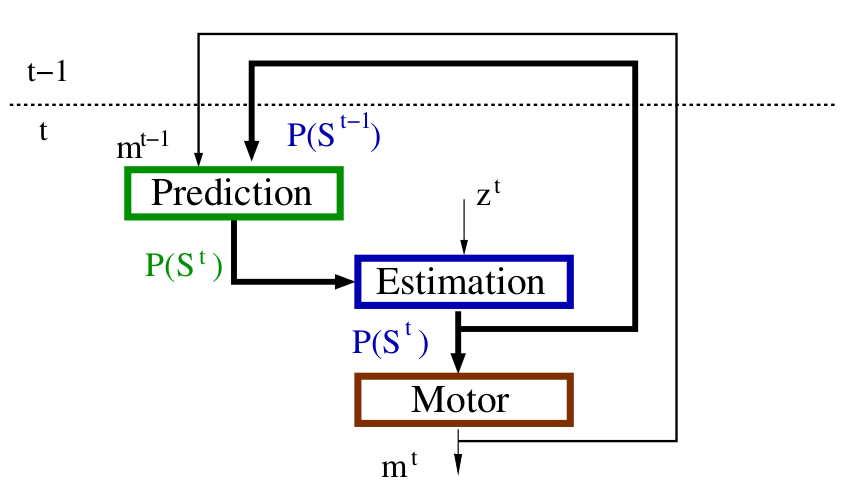
\includegraphics[width=120mm]{images/modelo_bayesiano-Carla}
    \caption{\label{img:ModeloProbabilisticoCarla}Filtro Bayesiano Recursivo. Fonte: \cite{INCA2005} [Trocar por tese da Carla]}
\end{figure}

Com essas densidades probabilísticas podemos decidir por uma estratégia de ação em qualquer instante de tempo utilizando a ação $ M^t = m $ que maximize essa função. Podemos também descobrir o estado mais provável de o sistema se encontrar fazendo a mesma coisa para $ S^j $.

Esse modelo pode, ainda, ser discretizado para cada instante de tempo, ficando:

\begin{equation}
        P ( M^{0: t} S^{0: t} Z^{0: t} \mid \pi_f ) = P ( M^{0: t-1} S^{0: t-1} Z^{0: t-1} \mid \pi_f ) \cdot 
        \left(
            \begin{array}{l}
                P( S^j \mid S^{j -1} M^{j -1} \pi_f ) \\
                \times P( Z^j \mid S^j \pi_f ) \\
                \times P( M^j \mid S^j M^{j -1} \pi_f )
            \end{array}
        \right)
\end{equation}

Com isso temos um modelo recursivo que pode ser chamado a cada instante de tempo para atualizar o modelo de probabilidades. Essa atualização pode ainda ser dividida em quatro partes distintas:

\subsection{Predição}

Nessa etapa, a partir da ação escolhida no período anterior de tempo, se faz uma estimativa de qual será o estado após sua execução.

\begin{equation}
    P \left( S^t \mid z^{0: t-1} m^{0: t-1} \pi_f \right) \propto \sum\limits_{S^{t-1}}
        \left(
            \begin{array}{l}
                P \left( S^t \mid S^{t-1} m^{t-1} \pi_f \right) \\
                \times P \left( m^{t-1} \mid S^{t-1} m^{t-2} \pi_f \right)\\
                \times P \left( S^{t-1} \mid z^{0: t-1} m^{0: t-2} \pi_f \right)
            \end{array}
        \right)
\end{equation}


\subsection{Observação}

Tendo, agora, um dos comportamentos escolhido, se atualiza o belief state do agente a partir dos sensores presentes no robô.

\begin{equation}
    P \left( S^t \mid z^{0: t} m^{0: t-1} \pi_i \right) \propto 
        \left(
            \begin{array}{l}
                P \left( z^t \mid S^t \pi_f \right) \\
                \times P \left( S^t \mid z^{0: t-1} m^{0: t-1} \pi_f \right)
            \end{array}
        \right)
\end{equation}


\subsection{Escolha de ação motor}

Por último se faz a seleção de uma ação a ser executada pelo robô de forma análoga à seleção de comportamentos. Calcula-se as probabilidade de se executar cada ação  e se escolhe a com maior valor.

\begin{equation}
    P \left( M^t \mid z^{0: t} m^{0: t-1} \pi_f \right) \propto \sum\limits_{S_i^t}
        \left(
            \begin{array}{l}
                \times P \left( M^t \mid S^t m^{t-1} \pi_f \right)\\
                \times P \left( S^t \mid z^{0: t} m^{0: t-1} \pi_f \right)
            \end{array}
        \right)
\end{equation}


\section{MDP (Processo de Decisão de Markov)} \label{section:MDP}

MDPs são utilizados em várias áreas, como economia, manufatura de processos e robótica. Ele foi nomeado a partir de Andrey Markov e provê uma base matemática para o modelamento de tomada de decisões. Eles são uma extensão de cadeias de Markov, tendo como diferença a adição de ações e recompensas (escolha e motivação).

MDP é, mais precisamente, um processo de controle estocástico de tempo discreto. O que isso significa é que ele é um processo de controle probabilístico, baseado em passos (time steps). Em cada passo o robô se encontra em um estado $ S $ perfeitamente conhecido em que pode-se executar qualquer ação $ u $ disponível para esse estado. O modelo de percepção do robô, $ p \left( Z \mid S \right) $ é uma equação determinística e bijetora, o robô só pode estar em um estado $ s \in S $ para uma percepção $ z \in Z $ do ambiente.

Após executada essa ação, o robô se encontrará em um novo estado $ s' \in S $ com probabilidade $ p \left( s' \mid u, s \right) $, essa equação é conhecida como modelo de atuação (action model). O modelo de atuação não é, em geral, determinístico, ou seja, uma ação pode ter várias consequências com diferentes probabilidades. Uma consequência disso é que planejar uma única sequência de ações não é o suficiente, o planejador de decidir por uma ação para cada um de uma gama de estados em que o robô pode se encontrar.

Considere o sistema de figura a seguir em que para uma dada ação A ou B tem-se indicada as probabilidades $ p \left( s' \mid u, s \right) $ através da percentagem indicada nas setas saindo do estado $ s $ para $ s' $.


\begin{figure}[h]
    \centering
    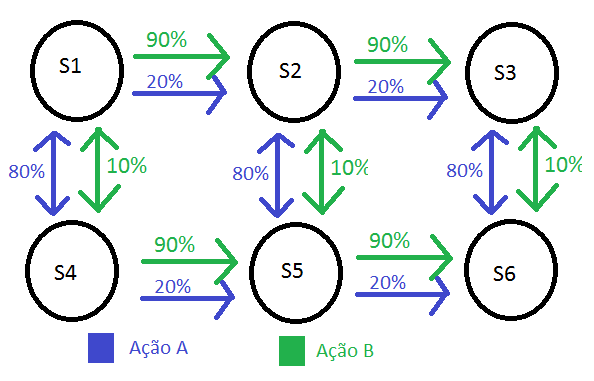
\includegraphics[width=120mm]{images/probabilidade-markov}
    \caption{\label{img:MapaDeProbabilidadesMarkov}Mapa de Probabilidades}
\end{figure}

Podemos, por exemplo, ver que para esse sistema $ P \left( s2 \mid a, s1 \right) = 0.2 $ e $ P \left( s4 \mid a, s1 \right) = 0.8 $. Se nós tivermos o estado $ s6 $ como objetivo, note que não adianta se obter uma sequência de ações $ a \rightarrow a \rightarrow b$, por exemplo, pois nós podemos nos encontrar em uma gama de estados ao final dessa sequência. Poderíamos nos encontrar em $ s4 $, $ s2 $ ou $ s6 $.

Temos então de mapear uma ação para cada estado possível em que pudermos nos encontrar, gerando o que é chamado de política de controle (control policy). Essa política de controle terá formato $ \pi: S_t \rightarrow U_t $, a política $ \pi $ recebe um estado e retorna a ação planejada para ele. Note então que, tendo essa política $ \pi \left( S \right) $, não temos problemas como no caso anterior, pois sempre teremos planejado que ação tomar em um dado instante, baseado no estado em que nos encontrarmos.

Calcular essa política não é um problema trivial, devido, entre outros motivos, à existência de infinitos caminhos para se chegar de um estado $ s1 $ a $ s6 $. Um caminho seria $ s1 \rightarrow s2 \rightarrow s3 \rightarrow s6 $, por exemplo, e outro seria $ s1 \rightarrow s2 \rightarrow s5 \rightarrow s2 \rightarrow s3 \rightarrow s6 $, outro ainda seria $ s1 \rightarrow s2 \rightarrow s5 \rightarrow s2 \rightarrow s5 \rightarrow s2 \rightarrow s3 \rightarrow s6 $.

Antes de poder obter um algoritmo definitivo, temos de modelar o que seria o objetivo de um problema. Para isso utilizaremos uma função de recompensa para o robô $ r \left( S, U, S' \right) $ que retorna um número real. Ela indica quão desejado é se chegar a uma estado $ s' $ a partir de $ s $ executando a ação $ u $. Para sistemas em que só se preocupe em chegar ao estado desejado pode-se simplifica-la para $ r \left( s' \right) $, por exemplo.

Sabendo que queremos achar uma política que maximize o ganho de recompensas podemos gerar um plano de políticas ótimo pensando-se apenas na próxima ação, maximizando uma recompensa imediata. Caso nossas recompensas fossem dadas apenas pela escolha de uma ação baseada no estado atual $ r \left( S, U \right) $ (sem considerar o estado alcançado) teríamos como escolha de política:

\begin{equation}
    \pi_1 \left( s \right) = \underset{u}{argmax} \left( r \left( s, u \right) \right)
\end{equation}

Como nossa recompensa depende também do estado alcançado, devemos pesar cada recompensa $ r \left( S, U, S' \right) $ pela probabilidade de se alcançar o estado $ S' $.

\begin{equation}
    \pi_1 \left( s \right) = \underset{u}{argmax} \left( \int \! r \left( s, u, s' \right) \cdot P \left( s' \mid u, s \right) \, \mathrm{d}s'. \right)
\end{equation}

Podemos gerar para essa política um função de valor (value function) que represente a recompensa esperada para cada estado $ s $ seguindo a política $ \pi $.

\begin{equation}
    V_1 \left( s \right) = \underset{u}{max} \left( \int \! r \left( s, u, s' \right) \cdot P \left( s' \mid u, s \right) \, \mathrm{d}s'. \right)
\end{equation}

Pensando no passo seguinte, podemos utilizar esse novo valor $ V_1 \left( S \right) $ para calcular uma política planejando agora um passo à frente e depois generalizar para qualquer caso futuro.

\begin{equation}
    \pi_t \left( s \right) = \underset{u}{argmax} \left( \int \! \left( r \left( s, u, s' \right) + \gamma \cdot V_{t-1} \left( s' \right) \right) \cdot P \left( s' \mid u, s \right) \, \mathrm{d}s'. \right)
\end{equation}

Sendo $ \gamma $ uma constante de desconto, usada para incentivar o ganho de recompensas imediatas à tardias. Essa função indica que a política ótima é a que gera uma maior recompensa imediata, somada com a somatória de todas as recompensas futuras esperadas ponderadas pelas probabilidades de serem recebidas. Podemos novamente gerar uma função de valor para essa política:

\begin{equation}
    V_t \left( s \right) = \underset{u}{max} \left( \int \! \left( r \left( s, u, s' \right) + \gamma \cdot V_{t-1} \left( s' \right) \right) \cdot P \left( s' \mid u, s \right) \, \mathrm{d}s'. \right)
\end{equation}

Para um tempo $ t = \infty $, a política geralmente converge e uma ótima para esse sistema é encontrada.

\begin{equation}
    \pi^* \left( s \right) = \pi_\infty \left( s \right) = \underset{u}{argmax} \left( \int \! \left( r \left( s, u, s' \right) + \gamma \cdot V_\infty \left( s' \right) \right) \cdot P \left( s' \mid u, s \right) \, \mathrm{d}s'. \right)
\end{equation}

\begin{equation} \label{equation:ValueFunctionMDP}
    V^* \left( s \right) = V_\infty \left( s \right) = \underset{u}{max} \left( \int \! \left( r \left( s, u, s' \right) + \gamma \cdot V_\infty \left( s' \right) \right) \cdot P \left( s' \mid u, s \right) \, \mathrm{d}s'. \right)
\end{equation}


\section{TD (Diferença Temporal)} \label{section:TD}

O que fazer se você não conhece os valores das recompensas $ r \left( S, U, S' \right) $ ou qual o resultado de uma ação $ P \left( s' \mid u, s \right) $? O algoritmo de diferença temporal visa, a partir de uma política fixa $ \pi \left( S \right) $, aprender os valores finais de $ V \left( S \right) $ através da execução de ações em diferentes estados, sem ter um conhecimento prévio das recompensas recebidas ou do modelo probabilístico do resultado de suas ações.

Esse algoritmo se baseia na equação \ref{equation:ValueFunctionMDP} obtida no seção \ref{section:MDP} e parte da premissa de que se tem uma política $ \pi_{td} $ já escolhida e fixa. Utilizando isso ele atualiza o valor de $ V \left( S \right) $ cada vez que experiencia um $ \left( s, u, s', r \right) $ qualquer, ou seja, que alcança um estado $ s' \in S $ a partir do estado $ s \in S $, com uma ação $ u \in U $ e recebendo uma recompensa $ r \in \mathbb{R} $. A partir de cada dessas experiências, pode-se obter um valor amostra tal que:

\begin{equation} \label{equation:AmostraTD}
	amostra = r \left( s, u, s' \right) + \gamma \cdot V_{\pi_{td}}^t \left( s' \right)
\end{equation}

Agora, escolhendo-se uma constante de aprendizagem $ \alpha $, pode-se atualizar o valor de $ V_{\pi_{td}} \left( s \right) $ tal que:

\begin{equation} \label{equation:UpdateValueFunctionTD}
	V_{\pi_{td}}^t \left( s \right) = \left( 1 - \alpha \right) \cdot V_{\pi_{td}}^{t-1} \left( s \right) + \alpha \cdot amostra
\end{equation}

Note que, utilizando valores suficientemente pequenos de $ \alpha $, consegue-se valores de $ V_{\pi_{td}} \left( s \right) $ que convergem com o tempo e que, mais importante, convergem para os mesmos valores que o algoritmo MDP, considerando que a política $ \pi_{td} $ utilizada é ótima.

O problema com a diferença temporal é que ela apenas avalia uma política fixa e já existente. Caso queiramos mudar nossa política, ou gerar uma utilizando esse algorítmo, teríamos um problema, todos os valores de $ V \left( S \right) $ dependem somento do estado e não da ação executada. Caso se mudasse a política $ \pi_{td} $ executada, teríamos de recalcular todos os valores $ V \left( S \right) $.

\section{Q Learning} \label{section:QLearning}

Q Learning é um dos mais conhecidos e mais utilizados algoritmos de aprendizagem por reforço, sendo utilizado para controle de robôs [adicionar ref], tratamento de problemas em processamento de imagens [adicionar ref] e criação de sistemas de troca financeiros [adicionar ref]. Esse é um algoritmo, diferentemente do TD, de aprendizagem ativa, ou seja, a escolha da política e das ações é feita juntamente com a aprendizagem e se consegue alcançar uma nova política ótima o utilizando.

Ao invés de utilizar o valor de $ V \left( S \right) $ e se basear na equação \ref{equation:ValueFunctionMDP}, ele utiliza um valor $ Q \left( S, U \right) $, tal que:

\begin{equation} \label{equation:PolicySelectionQLearning}
    \pi^t \left( s \right) = \underset{u}{argmax} \left( Q^t \left( s, u \right) \right)
\end{equation}

\begin{equation}
    V^t \left( s \right) = \underset{u}{max} \left( Q^t \left( s, u \right) \right)
\end{equation}

Ou seja:

\begin{equation} \label{equation:QValueFunctionQLearning}
    Q^t \left( s, u \right) = \int \! \left( r \left( s, u, s' \right) + \gamma \cdot V^{t-1} \left( s' \right) \right) \cdot P \left( s' \mid u, s \right) \, \mathrm{d}s'
\end{equation}

Que pode ser reescrito como:

\begin{equation} \label{equation:QValueFunctionQLearningFinal}
    Q^t \left( s, u \right) = \int \! \left( r \left( s, u, s' \right) + \gamma \cdot \underset{u'}{max} \left( Q^{t-1} \left( s', u' \right) \right) \right) \cdot P \left( s' \mid u, s \right) \, \mathrm{d}s'
\end{equation}

Ao aprender o valor de $ Q^t \left( S, U \right) $, ao invés do de $ V^t \left( S \right) $, você pode modificar sua política sem ter que reaprender todos os seus valores. Analogamente às equações \ref{equation:AmostraTD} e \ref{equation:UpdateValueFunctionTD} em TD, aprende-se através de amostras obtidas a partir de experiências $ \left( s, u, s', r \right) $.


\begin{equation}
	amostra = r \left( s, u, s' \right) + \gamma \cdot \underset{u}{max} \left( Q^{t-1} \left( s', u' \right) \right)
\end{equation}

\begin{equation}
	Q^t \left( s, u \right) = \left( 1 - \alpha \right) \cdot Q^{t-1} \left( s, u \right) + \alpha \cdot amostra
\end{equation}

Com um número suficiente de iterações e com um decaimento apropriado do parâmetro de aprendizagem $ \alpha $, $ Q^t \left( S, U \right) $ tende a um valor ótimo  com uma probabilidade 1 [adicionar refs convergência de q] e uma política escolhida com base na função \ref{equation:PolicySelectionQLearning} também seria ótima.

Alguns problemas com esse algoritmo são:

\begin{itemize}
	\item Podem existir muitos estados para se visitar, para um espaço contínuo, por exemplo, seriam infinitos;
	\item Podem existir muitas ações possíveis para cada estado, para o acionamento analógico de um motor, por exemplo, seriam infinitas;
	\item Se houverem muitos pares ação-estado $ \left( S, U \right) $, mesmo que se consiga aprender por um tempo muito grande, tem que se conseguir armazenar o valor de $ Q_t \left( S, U \right) $ para cada ação que for possível de ser executada em cada estado;
	\item O algoritmo não consegue aplicar o que aprendeu em um estado para outros com características parecidas.
\end{itemize}

\subsection{Generalização dos Pares Estado-Ação}

Uma solução para esse problema é generalizar a informação de um par estado-ação para outros similares. Para isso utilizaremos um vetor de características $ f $ para descrever o estado. Essas características podem ser coisas como:

\begin{itemize}
	\item Distância para uma posição que oferece uma recompensa positiva;
	\item Distância para uma posição que oferece uma recompensa negativa;
	\item Número de alvos a serem capturados;
	\item Estado do robô (Com ou sem problema).
\end{itemize}

Essas características podem descrever também a ação a ser executada, como:

\begin{itemize}
	\item Captura um alvo;
	\item Economiza energia.
\end{itemize}

Podemos utilizar esse vetor de características $ f_j \left( S, U \right) $ para obter um valor $ Q \left( S, U \right) $ tal que:

\begin{equation}
	Q \left( S, U \right) = \omega_1 \cdot f_1 \left( S, U \right) + \omega_2 \cdot f_2 \left( S, U \right) + \cdots + \omega_n \cdot f_n \left( S, U \right)
\end{equation}

Com essa equação conseguimos um valor parecido de $ Q \left( S, U \right) $ para estados distintos que possuam características $ f_j \left( S, U \right) $ com valores parecidos. A desvantagem é que devemos escolher esses valores/características com cuidado para obter uma boa representação do nosso par estado-ação a partir deles, ou podemos ter estados-ações com valores de $ f_j \left( S, U \right)$ parecidos, e, consequentemente, valores de $ Q \left( S, U \right) $ também parecidos, mas que são muito diferentes.

Com esse novo modelo, podemos aprender valores, a partir de cada experiência, utilizando o erro atual do modelo:

\begin{equation}
	erro = r \left( s, u, s' \right) + \gamma \cdot \underset{u}{max} \left( Q^{t-1} \left( s', u' \right) \right) - Q^{t-1} \left( s, u \right)
\end{equation}

Dada pela diferença entre a recompensa recebida somada com o valor de ganho esperado para o novo estado alcançado e o valor atual esperado para o par estado-ação executada. E o utilizando para atualizar cada um dos pesos usados para obter $ Q_t \left( S, U \right) $:

\begin{equation}
	\omega_i^t = \omega_i^{t-1} + \alpha \cdot erro \cdot f_i \left( s, u \right)
\end{equation}

Assim, caso tenhamos um erro grande para um dado estado, iremos atualizar os valores de todos os estados com características similares àquele. É importante notar também que, caso esse estado tenha um valor maior para uma das características $ f_j $, o peso dela, $ \omega_j $, será mais modificado que os da outras características.

Note que a função utilizada para calcular $ Q \left( S, U \right) $ é um perceptron e que esse tipo de função possuí limitações, sendo a principal a de ser capaz de aprender apenas problemas linearmente separáveis [ref perceptron limitations]. Por isso os parâmetros $ f_i \left( S, U \right) $ devem ser bem escolhidos, não só para caracterizar bem um estado e permitir uma boa diferenciação entre dois deles, mas também para permitir essa aprendizagem.




\begin{comment}
Desenvolvimento
\end{comment}
%TCIDATA{LaTeXparent=0,0,relatorio.tex}



\chapter{Desenvolvimento} \label{chap:Desenvolvimento}

% Resumo opcional. Comentar se não usar.
\resumodocapitulo{``Só sei que nada sei'' -- Sócrates}

\section{Introdução}

Este capítulo apresenta as soluções adotadas para os problemas de planejamento de tarefas e de tomada de decisões, bem como sua modelagem matemática. Nele também são descritos os ambientes de teste em simulação e a modelagem utilizada para descrever o agente móvel. Por último, ainda neste capítulo, é apresentada uma descrição dos testes realizados.

\section{Modelagem Matemática}

Nesta seção são descritas as mudanças realizadas nos modelos matemáticos utilizados nesse projeto. Também é apresentada uma explicação sobre o modelo final do projeto e sobre como as várias teorias se encaixam.

\subsection{Aprendizagem por Reforço para Seleção de Comportamentos} \label{subsection:QLearningSelecaoDeComportamento}

Um comportamento pode ser descrito como um conjunto de reações à estimulos externos, ou seja, ele é um modelo que um agente, ou sistema, utiliza para fazer a escolha de suas ações. Um agente, em um mesmo estado do sistema, pode ter duas escolhas de ação diferentes, se estiver em comportamentos diferentes.

Neste trabalho, a aprendizagem por reforço é utilizada para aprender uma política de seleção de comportamento e não de ações motoras. Para isso, é necessário alterar as equações do algoritmo \textit{Q Learning} para que, ao invés de escolher uma ação $ u \in U $, escolher um comportamento $ b \in B $. Reescrevendo as principais equações desse algoritmo elas são:

\begin{equation} \label{equation:QValueFunctionBehavior}
    Q^t \left( s, b \right) = \int \! \left( r \left( s, b, s' \right) + \gamma \cdot V^{t-1} \left( s' \right) \right) \cdot P \left( s' \mid b, s \right) \, \mathrm{d}s',
\end{equation}

\begin{equation} \label{equation:PolicySelectionBehavior}
    \pi^t \left( s \right) = \underset{b}{argmax} \left( Q^t \left( s, b \right) \right), e
\end{equation}

\begin{equation}
    V^t \left( s \right) = \underset{b}{max} \left( Q^t \left( s, b \right) \right).
\end{equation}

Além disso, as características $ f_j $ agora são ser baseadas em pares estado-comportamento $ \left( S, B \right) $ e não mais em pares estado-ação.

\begin{equation}
	Q \left( S, B \right) = \omega_1 \cdot f_1 \left( S, B \right) + \omega_2 \cdot f_2 \left( S, B \right) + \cdots + \omega_n \cdot f_n \left( S, B \right),
\end{equation}

\begin{equation} \label{equation:QErrorBehavior}
	erro = r \left( s, b, s' \right) + \gamma \cdot \underset{b}{max} \left( Q^{t-1} \left( s', b' \right) \right) - Q^{t-1} \left( s, b \right), e
\end{equation}

\begin{equation} \label{equation:OmegaUpdateBehavior}
	\omega_i^t = \omega_i^{t-1} + \alpha \cdot erro \cdot f_i \left( s, b \right).
\end{equation}


\subsection{Seleção de Comportamentos em um Sistema Parcialmente Observável} \label{subsection:QLearningParcialmenteObservavel}

O algoritmo \textit{Q Learning} foi criado baseado no MDP, que, como citado na seção \ref{section:MDP}, é utilizado para sistemas completamente observáveis%
\footnote{Sistemas em que existe uma função $ f \left( Z \right) $ que, dado uma medida dos sensores, retorna o estado atual do sistema. Em outras palavras, é um sistema em que, dado uma medida $ z \in Z $ dos sensores se sabe, sem dúvidas, qual o estado presente do sistema $ s \in S $%
}. É necessário, então, expandir sua definição para aplicá-lo em um sistema parcialmente observável%
\footnote{Sistema que não é completamente observável, ou seja, que para uma medida $ z \in Z $ dos sensores só se pode estimar qual a probabilidade desse sistema se encontrar num estado $ s \in S $%
}.

Para isso, deve-se primeiramente introduzir uma nova variável $ a \in A $ que representa a distribuição de probabilidades em todos os possíveis estados $ S $. Considere, por exemplo, um caso em que o vetor de estados seja composto por duas variáveis $ S = \binom{S_1}{S_2} $, que podem ter valores $ S_1 \in \left\{1,2,3\right\} $ e $ S_2 \in \left\{verdadeiro, falso\right\} $. Uma variável $ a \in A $, nesse caso, seria dada por cinco variáveis, representando as probabilidades de S ter cada um dos possíveis valores.

$$
	A = \left(
	\begin{matrix}
		P \left( S_1 = 1 \right) & P \left( S_2 = verdadeiro \right) \\
		P \left( S_1 = 2 \right) & P \left( S_2 = falso \right) \\
		P \left( S_1 = 3 \right) &  
	\end{matrix} \right)
$$

A partir dessa definição, utilizando como inspiração o algoritmo POMDP \cite{Thrun:2005:PR:1121596}, o estado $ s \in S $ é substituido, na equação \ref{equation:QValueFunctionQLearning}, por uma variável $ a \in A $, que represente essa distribuição de probabilidades nos possíveis estados $ S $.

\begin{equation} \label{equation:QValueFunctionPartiallyObservable}
    Q^t \left( a, b \right) = \int \! \left( r \left( a, b, a' \right) + \gamma \cdot V^{t-1} \left( a' \right) \right) \cdot P \left( a' \mid b, a \right) \, \mathrm{d}a'.
\end{equation}

Tem-se, agora, uma seleção de política baseada na distribuição de probabilidades nos estados $ s \in S $:

\begin{equation} \label{equation:PolicySelectionPartiallyObservable}
    \pi^t \left( a \right) = \underset{b}{argmax} \left( Q^t \left( a, b \right) \right),
\end{equation}

\begin{equation}
    V^t \left( a \right) = \underset{b}{max} \left( Q^t \left( a, b \right) \right).
\end{equation}


Analogamente às equações \ref{equation:AmostraQLearning} e \ref{equation:QUpdateQLearning} no \textit{Q Learning} original, aprende-se através de amostras obtidas a partir de experiências $ \left( a, b, a', r \right) $.


\begin{equation}
	amostra = r \left( a, b, a' \right) + \gamma \cdot \underset{b}{max} \left( Q^{t-1} \left( a', b' \right) \right),
\end{equation}

\begin{equation}
	Q^t \left( a, b \right) = \left( 1 - \alpha \right) \cdot Q^{t-1} \left( a, b \right) + \alpha \cdot amostra.
\end{equation}

O problema dessa equação é que, ao utilizar um espectro $ a \in A $ de probabilidades de todos os estados $ s \in S $ e não próprio estado, não é possível simplesmente aprender os valores para cada item. Isso acontece pois, mesmo para espaços de estados discretos, há infinitos valores de $ a \in A $ possíveis.

A teoria vista no tópico \ref{subsection:GeneralizaçãoParesEstadoAção} é utilizada, então, para criar uma generalização desses estados através de características deles. Essas características, ao contrário das vistas anteriormente, devem ser baseadas nas probabilidades de se estar/alcançar um estado. Alguns exemplos são:

\begin{itemize}
	\item Distância da posição mais provável do robô, para uma posição que ofereça um produto ( probabilidade de receber uma recompensa * recompensa ) alta;
	\item Distância da posição mais provável do robô, para uma posição que ofereça um produto ( probabilidade de receber uma recompensa * recompensa ) negativa;
	\item Probabilidade de existir algum perigo (recompensa negativa) a menos que uma certa distância;
	\item Probabilidade de capturar um alvo;
	\item Porcentagem de chance do robô ter um erro.
\end{itemize}

Essas características podem, como no caso anterior, descrever também o comportamento a ser executado, como:

\begin{itemize}
	\item Tentar capturar um alvo;
	\item Tentar fugir de um perigo;
	\item Economizar energia.
\end{itemize}

Com isso um valor $ Q \left( A, B \right) $ é obtido, tal como descrito na equação \ref{equation:QValueFinal1}.

\begin{equation} \label{equation:QValueFinal1}
	Q \left( A, B \right) = \omega_1 \cdot f_1 \left( A, B \right) + \omega_2 \cdot f_2 \left( A, B \right) + \cdots + \omega_n \cdot f_n \left( A, B \right).
\end{equation}


Com esse novo modelo, é possível aprender valores, a partir de cada experiência, utilizando o erro atual do sistema:

\begin{equation} \label{equation:ErroQPartiallyObservable}
	erro = r \left( a, b, a' \right) + \gamma \cdot \underset{b}{max} \left( Q^{t-1} \left( a', b' \right) \right) - Q^{t-1} \left( a, b \right).
\end{equation}
e o utilizando para atualizar cada um dos pesos usados para obter $ Q^t \left( A, B \right) $:
\begin{equation} \label{equation:UpdateOmegaQPartiallyObservable}
	\omega_i^t = \omega_i^{t-1} + \alpha \cdot erro \cdot f_i \left( a, b \right).
\end{equation}

Assim, caso exista um erro grande para um dado espectro de probabilidades, são atualizados os valores de todos os casos que possuam espectros de probabilidades dos estados com características similares àquele. E caso esse estado tenha um valor maior para uma das características, o peso dela será mais modificado que as outras.

Então, caso for utilizada como característica, por exemplo, $ f_i = $ ``probabilidade de existir algum perigo (recompensa negativa) a menos que uma certa distância''. Se for recebida uma recompensa negativa em um estado no qual o valor de $ f_i $ é alto, estados com essa característica serão considerados piores. Se for recebida uma recompensa positiva, os estados com valor alto para essa característica serão considerados melhores.


\subsection{Abordagem Bayesiana com a Seleção de Comportamentos} \label{subsection:BayesComSelecaoDeComportamento}

Partindo dos modelos obtidos na seção \ref{section:FiltroBayesiano}, pode-se agora utilizar a seleção de comportamento, vista no tópico \ref{subsection:QLearningParcialmenteObservavel}, como uma nova medida de sensor, fazendo:

\begin{equation}
	Z' = \binom{Z}{Z_b} = \binom{Z}{B}.
\end{equation}

Sendo $ Z $ as medidas sensorias e $ B = Z_b $ o comportamento obtido utilizando a aprendizagem por reforço. É necessário expandir também o modelo dos estados para:

\begin{equation}
	S' = \binom{S}{S_b}
\end{equation}

Sendo, novamente, $ S $ o modelo do estado atual usual e $ S_b $ uma variável de estado que representa o comportamento atual do agente.

O filtro bayesiano é, então, reescrito como:

\begin{equation}
        P \left( M^{0: t} S^{0: t} S_b^{0: t} Z^{0: t} B^{0: t} \mid \pi_f \right) = P \left( M^0 S^0 S_b^0 Z^0 B^0 \mid \pi_f \right) \cdot \prod\limits_{j =1}^{t} 
        \left(
            \begin{array}{l}
                P \left( S^j S_b^j \mid S^{j -1} S_b^{j-1} M^{j -1} \pi_f \right) \\
                \times P \left( Z^j B^j \mid S^j S_b^{j-1} \pi_f \right) \\
                \times P \left( M^j \mid S^j S_b^j M^{j -1} \pi_f \right)
            \end{array}
        \right).
\end{equation}

Existem três etapas para atualizar o estado $ S'^t $ recursivamente. Para esse novo filtro elas são:

\begin{itemize}
	\item Predição:
		\begin{equation}
    P \left( S^t S_b^t \mid z^{0: t-1} b^{0: t-1} m^{0: t-1} \pi_f \right) \propto \sum\limits_{S^{t-1} S_b^{t-1}}
        \left(
            \begin{array}{l}
                P \left( S^t S_b^t \mid S^{t-1} S_b^{t-1}  m^{t-1} \pi_f \right) \\
                \times P \left( m^{t-1} \mid S^{t-1} S_b^{t-1} m^{t-2} \pi_f \right)\\
                \times P \left( S^{t-1} S_b^{t-1} \mid z^{0: t-1} b^{0: t-1} m^{0: t-2} \pi_f \right)
            \end{array}
        \right);
		\end{equation}
	\item Observação:
		\begin{equation}
    P \left( S^t S_b^t \mid z^{0: t} b^{0: t} m^{0: t-1} \pi_f \right) \propto
        \left(
            \begin{array}{l}
                P \left( z^t b^t \mid S^t S_b^t \pi_f \right) \\
                \times P \left( S^t S_b^t \mid z^{0: t-1} b^{0: t-1} m^{0: t-1} \pi_f \right)
            \end{array}
        \right);
		\end{equation}
	\item Seleção de ação motora:
		\begin{equation}
    P \left( M^t \mid z^{0: t} b^{0: t} m^{0: t-1} \pi_f \right) \propto \sum\limits_{S_i^{t-1} S_b^{t-1}}
        \left(
            \begin{array}{l}
                P \left( M^t \mid S^t S_b^t m^{t-1} \pi_f \right)\\
                \times P \left( S^t S_b^t \mid z^{0: t} b^{0: t} m^{0: t-1} \pi_f \right)
            \end{array}
        \right).
		\end{equation}
\end{itemize}

Assume-se que o estado $ S^t $ é independente do comportamento sendo executado no mesmo momento $ S_b^t $ e que esse comportamento atual independe de tempos anteriores. Assume-se, também, que os dados sensoriais $ Z^t $ são independentes do comportamento escolhido pelo \textit{Q Learning} ($ B^t $) num mesmo momento. Com isso, é possível simplificar o filtro para:

\begin{equation}
	\begin{split}
        P \left( M^{0: t} S^{0: t} S_b^{0: t} Z^{0: t} B^{0: t} \mid \pi_f \right) = \\
        		P \left( M^0 S^0 S_b^0 Z^0 B^0 \mid \pi_f \right) \cdot \prod\limits_{j =1}^{t} 
        &\left(
            \begin{array}{l}
                P \left( S^j \mid S^{j -1} M^{j -1} \pi_f \right) \times P \left( S_b^j \mid \pi_f \right) \\
                \times P \left( Z^j \mid S^j \pi_f \right) \times P \left( B^j \mid S_b^{j-1} \pi_f \right) \\
                \times P \left( M^j \mid S^j S_b^j M^{j -1} \pi_f \right)
            \end{array}
        \right).
	\end{split}
\end{equation}


Pode-se perceber que o modelo de seleção de ação motora:
\begin{equation}
	P \left( M^t \mid S^t S_b^t M^{t-1} \pi_f \right),
\end{equation}
agora depende do comportamento sendo utilizado.

\begin{equation}
    P \left( M^t \mid S^t S_b^t M^{t-1} \pi_f \right) = 
        \left\{
            \begin{array}{l}
                P \left( M^t \mid S^t \left[ S_b^t=b_1 \right] M^{t-1} \pi \right) \\
                P \left( M^t \mid S^t \left[ S_b^t=b_2 \right] M^{t-1} \pi \right) \\
                \cdots \\
                P \left( M^t \mid S^t \left[ S_b^t=b_{N_b} \right] M^{t-1} \pi \right)
            \end{array}.
        \right.
\end{equation}

A vantagem é que pode-se ter, para cada comportamento, um modelo de ação diferente. Esse modelo pode ainda ser escrito em sua forma recursiva, para um dado instante de tempo $ t $, ficando como na equação \ref{equation:BayesianModelFinalRecursivo}.
\begin{equation} \label{equation:BayesianModelFinalRecursivo}
	\begin{split}
        P \left( M^{0: t} S^{0: t} S_b^{0: t} Z^{0: t} B^{0: t} \mid \pi_f \right) = \\
        		P \left( M^{0: t-1} S^{0: t-1} S_b^{0: t-1} Z^{0: t-1} B^{0: t-1} \mid \pi_f \right) \cdot 
        &\left(
            \begin{array}{l}
                P \left( S^t \mid S^{t -1} M^{t -1} \pi_f \right) \times P \left( S_b^t \mid \pi_f \right) \\
                \times P \left( Z^t \mid S^t \pi_f \right) \times P \left( B^t \mid S_b^{t-1} \pi_f \right) \\
                \times P \left( M^t \mid S^t S_b^t M^{t -1} \pi_f \right)
            \end{array}
        \right).
	\end{split}
\end{equation}

Esse filtro simplificado pode, como o na seção \ref{section:FiltroBayesiano}, ser escrito na sua forma recursiva e separado em 3 etapas.

\begin{itemize}
	\item Predição:
		\begin{equation}
    P \left( S^t S_b^t \mid z^{0: t-1} b^{0: t-1} m^{0: t-1} \pi_f \right) \propto \sum\limits_{S^{t-1} S_b^{t-1}}
        \left(
            \begin{array}{l}
                P \left( S^t \mid S^{t-1} m^{t-1} \pi_f \right) \times P \left( S_b^t \mid \pi_f \right) \\
                \times P \left( m^{t-1} \mid S^{t-1} S_b^{t-1} m^{t-2} \pi_f \right)\\
                \times P \left( S^{t-1} S_b^{t-1} \mid z^{0: t-1} b^{0: t-1} m^{0: t-2} \pi_f \right)
            \end{array}
        \right);
		\end{equation}
	\item Observação:
		\begin{equation}
    P \left( S^t S_b^t \mid z^{0: t} b^{0: t} m^{0: t-1} \pi_f \right) \propto
        \left(
            \begin{array}{l}
                P \left( z^t \mid S^t \pi_f \right) \times P \left( b^t \mid S_b^t \pi_f \right) \\
                \times P \left( S^t S_b^t \mid z^{0: t-1} b^{0: t-1} m^{0: t-1} \pi_f \right)
            \end{array}
        \right);
		\end{equation}
	\item Seleção de ação motora:
		\begin{equation}
    P \left( M^t \mid z^{0: t} b^{0: t} m^{0: t-1} \pi_f \right) \propto \sum\limits_{S^{t-1} S_b^{t-1}}
        \left(
            \begin{array}{l}
                P \left( M^t \mid S^t S_b^t m^{t-1} \pi_f \right)\\
                \times P \left( S^t S_b^t \mid z^{0: t} b^{0: t} m^{0: t-1} \pi_f \right)
            \end{array}
        \right).
		\end{equation}
\end{itemize}


\subsection{Modelo Final e Completo}

Em posse da modelagem matemática introduzida no capítulo \ref{chap:FundamentacaoMatematica} e explorada nos tópicos \ref{subsection:QLearningSelecaoDeComportamento}, \ref{subsection:QLearningParcialmenteObservavel} e \ref{subsection:BayesComSelecaoDeComportamento} é possível agora apresentar o modelo completo utilizado neste trabalho.

É possível separar esse modelo em duas partes: uma de treinamento e outra em que a aprendizagem já foi comcluída.

Durante a fase de treinamento, então, um modelo com cinco etapas é utilizado. As já conhecidas: predição; observação; seleção de ação motora. Integradas com a seleção de comportamento e aprendizagem. Esse modelo está representado na figura \ref{img:ModeloFinalTreinamento}.

\begin{figure}[H]
    \centering
    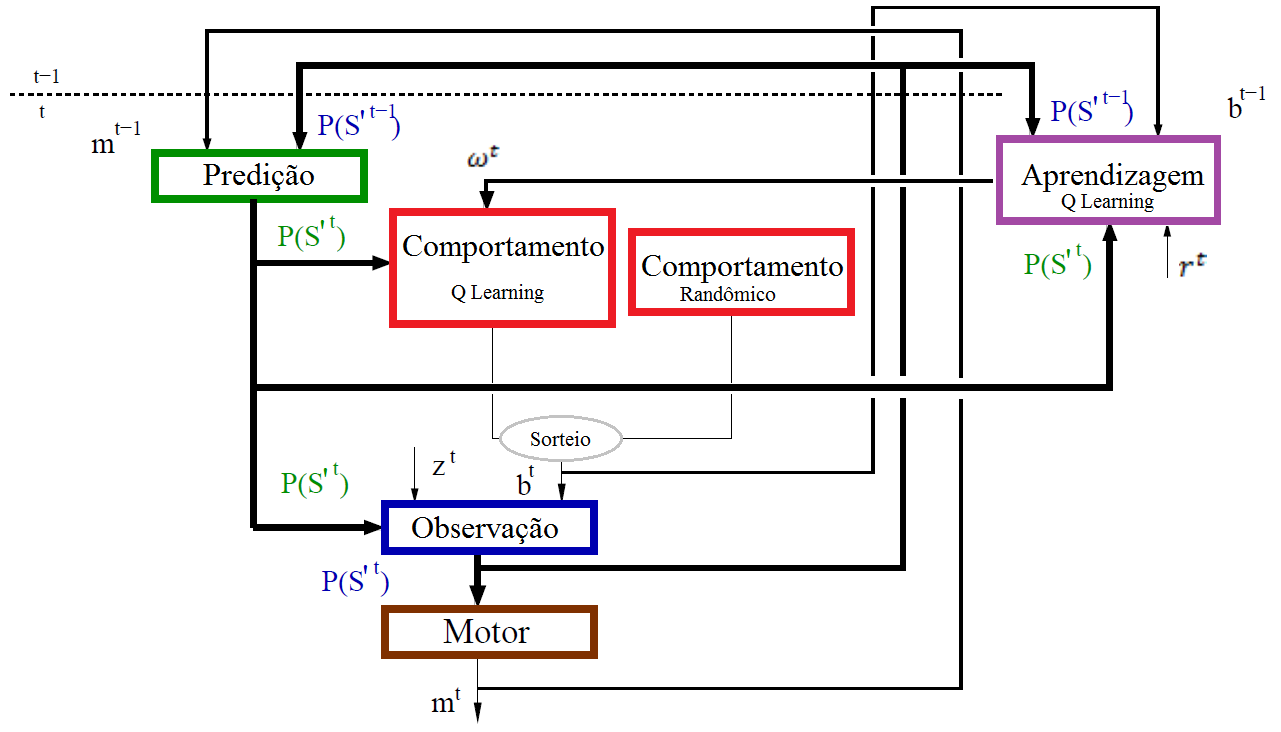
\includegraphics[width=150mm]{images/modelo_bayesiano_treino-tiago}
    \caption{Filtro Bayesiano utilizando \textit{Q Learning} para Seleção de Comportamento. Durante treinamento.}
    \label{img:ModeloFinalTreinamento}
\end{figure}

Após acabado o treinamento, não se tem mais necessidade da etapa de aprendizagem, ficando então um modelo com apenas 4 etapas. Esse modelo pode ser representado pela figura \ref{img:ModeloFinalPosTreinamento}.

\begin{figure}[h!]
    \centering
    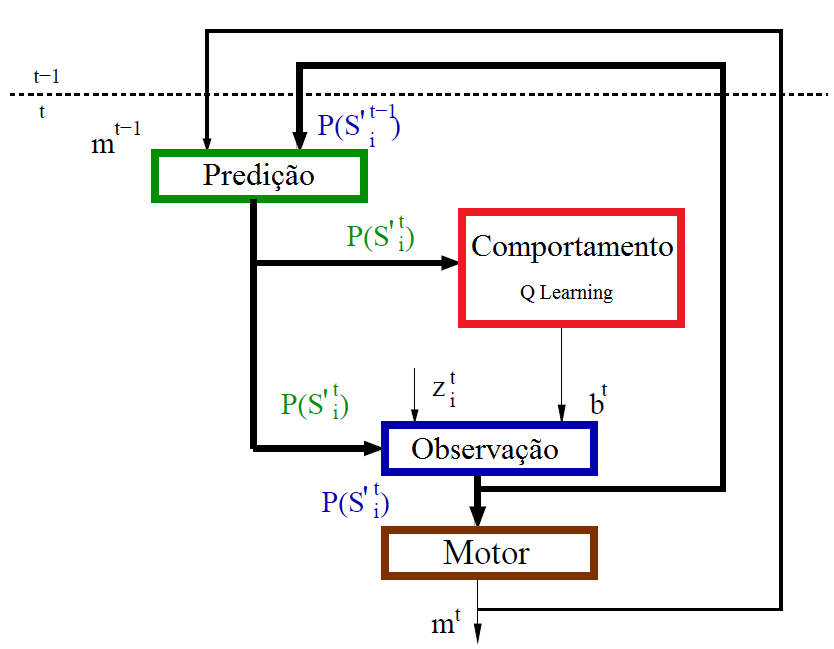
\includegraphics[width=120mm]{images/modelo_bayesiano_final-tiago}
    \caption{Filtro Bayesiano utilizando \textit{Q Learning} para Seleção de Comportamento. Após treinamento completo.}
    \label{img:ModeloFinalPosTreinamento}
\end{figure}

\subsubsection{Predição} \label{subsubsection:ModeloFinalPredicao}

Nessa etapa, a partir da ação escolhida no período anterior de tempo (instante de tempo $ t-1 $), se faz uma estimativa de qual será o estado após sua execução (instante de tempo $ t $).

\begin{equation}
    P \left( S^t S_b^t \mid z^{0: t-1} b^{0: t-1} m^{0: t-1} \pi_f \right) \propto \sum\limits_{S^{t-1} S_b^{t-1}}
        \left(
            \begin{array}{l}
                P \left( S^t \mid S^{t-1} m^{t-1} \pi_f \right) \times P \left( S_b^t \mid \pi_f \right) \\
                \times P \left( m^{t-1} \mid S^{t-1} S_b^{t-1} m^{t-2} \pi_f \right)\\
                \times P \left( S^{t-1} S_b^{t-1} \mid z^{0: t-1} b^{0: t-1} m^{0: t-2} \pi_f \right)
            \end{array}
        \right).
\end{equation}


\subsubsection{Escolha de comportamento}

Essa etapa é onde a escolha do comportamento acontece. Ela pode ter dois métodos distintos, um durante a fase de treinamento e outro após acabar a aprendizagem.

Durante a aprendizagem se utiliza uma exploração gulosa, descrita no tópico \ref{subsection:EscolhaDeAçõesExploraçãoGulosa}, para fazer essa escolha do comportamento. Nela, primeiro se sorteia um número randômico $ x \in [0,1] $. Se esse número for menor que um fator de exploração $ \gamma $, se escolhe um comportamento randômico entre todos os possíveis. No caso contrário, se escolhe um comportamento da mesma forma que após a aprendizagem ter acabado, descrito a seguir.

Para a escolha de comportamento após terminado o treinamento, primeiro se calcula a função \ref{equation:QLearningEscolhaComportamentoFinal}, à seguir, para cada comportamento $ b \in B^t $ e para o conjunto de probabilidades%
\footnote{É importante ressaltar que $ a^t $ equivale ao conjunto de probabilidades $ P \left( S^t S_b^t \mid z^{0: t-1} b^{0: t-1} m^{0: t-1} \pi_f \right) $, obtido em \ref{subsubsection:ModeloFinalPredicao}.%
} $ a^t \in A^t $ de se encontrar em cada estado $ S^t $.

\begin{equation} \label{equation:QLearningEscolhaComportamentoFinal}
    	Q \left( a^t, B^t \right) = \omega^1 \cdot f^1 \left( a^t, B^t \right) + \omega^2 \cdot f^2 \left( a^t, B^t \right) + \cdots + \omega^n \cdot f^n \left( a^t, B^t \right)
\end{equation}

Depois, se escolhe um comportamento a partir desses valores calculados, sendo escolhido o que maximiza essa função.


\subsubsection{Observação}

A partir dos sensores presentes no robô e do valor $ b \in B $, obtido com o algoritmo de aprendizado, se atualiza o estado probabilístico (\textit{belief state}) do agente.

\begin{equation}
    P \left( S^t S_b^t \mid z^{0: t} b^{0: t} m^{0: t-1} \pi_f \right) \propto
        \left(
            \begin{array}{l}
                P \left( z^t \mid S^t \pi_f \right) \times P \left( b^t \mid S_b^t \pi_f \right) \\
                \times P \left( S^t S_b^t \mid z^{0: t-1} b^{0: t-1} m^{0: t-1} \pi_f \right)
            \end{array}
        \right).
\end{equation}


\subsubsection{Escolha de ação motora}

Por último se faz a seleção de uma ação a ser executada pelo robô. Para isso, calcula-se a distribuição de probabilidade de se executar cada ação $ m^t \in M^t $ e se escolhe a ação que possui maior valor nessa distribuição.

\begin{equation}
    P \left( M^t \mid z^{0: t} b^{0: t} m^{0: t-1} \pi_f \right) \propto \sum\limits_{S^t S_b^t}
        \left(
            \begin{array}{l}
                P \left( M^t \mid S^t S_b^t m^{t-1} \pi_f \right)\\
                \times P \left( S^t S_b^t \mid z^{0: t} b^{0: t} m^{0: t-1} \pi_f \right)
            \end{array}
        \right)
\end{equation}


\subsubsection{Aprendizagem}

Nessa etapa são atualizados os valores do modelo de seleção de comportamento $ Q \left( A, B \right) $ a partir de uma recompensa $ r $ recebida. Tendo posse dessa recompensa, da distribuição de probabilidades do estado anterior $ a^{t-1} \in A^{t-1} $ e atual $ a^t \in A^t $ do sistema e de qual o comportamento $ b^{t-1} \in B^{t-1} $ escolhido no tempo anterior pelo algoritmo de aprendizagem, é possível atualizar os pesos $ \omega_i $ do sistema de aprendizagem, como descrito nas equações \ref{equation:ErroQPartiallyObservable} e \ref{equation:UpdateOmegaQPartiallyObservable}, reescritas aqui por conveniência.

$$
	erro = r \left( a, b, a' \right) + \gamma \cdot \underset{b}{max} \left( Q^{t-1} \left( a', b' \right) \right) - Q^{t-1} \left( a, b \right)
$$

$$
	\omega_i^t = \omega_i^{t-1} + \alpha \cdot erro \cdot f_i \left( a, b \right)
$$



\section{Ambiente de Testes e Simulação} \label{section:AmbienteDeTestes}

Para poder testar as teorias aqui descritas foi utilizado uma plataforma de Pacman%
\footnote{Essa plataforma pode ser encontrada em http://ai.berkeley.edu/project\_overview.html%
}, criada em Berkeley para suas aulas de inteligência artificial.

\begin{figure}[h]
    \centering
    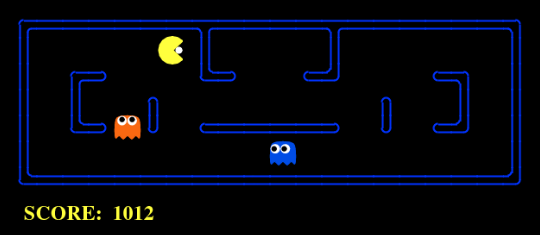
\includegraphics[width=120mm]{images/pacman_platform}
    \caption{\label{img:PlataformaSimulacaoPacman}Plataforma do jogo Pacman desenvolvida em Berkeley para aulas de IA.}
\end{figure}

A plataforma provê um sistema com informação completa%
\footnote{Todas as propriedades do jogo são conhecidas a todo momento, como por exemplo: posição do Pacman, posição dos fantasmas e localizações com ou se comida.%
} e sem erros na movimentação%
\footnote{Uma ação executada em um dado estado do sistema terá sempre o mesmo resultado.%
}. Essa plataforma foi programada em python e integrada com ROS \cite{ROS:1448}. Utilizando o ROS essa plataforma foi conectada com um programa em C++, no qual foi programado o modelo de aprendizagem e seleção de comportamento proposto neste trabalho.

A comunicação entre a plataforma em Python e o programa em C++ se dá a partir de quatro mensagens diferentes, as quais simulam os sensores, atuadores e recompensas do sistema.

\begin{itemize}
	\item Posição do agente (Pacman) --- $ \left( x, y \right) \in \mathbb{R}^2 $;
	\item Distância para os fantasmas --- $ \left( d_x, d_y \right) = \left( \Delta x, \Delta y \right) \in \mathbb{R}^2 $;
	\item Ação a ser executada --- $ u \in \left\{Norte, Sul, Leste, Oeste, Esperar \right\} $;
	\item Recompensa recebida do ambiente --- $ r \in \mathbb{R} $.
\end{itemize}

Para simular erros de sensoriamento, comuns em aplicações de robótica móvel, antes de enviar essas informações são inseridos erros Gaussianos tanto na posição do agente (Pacman), quanto nas distâncias para os fantasmas.

$$
	\left( x, y \right) = \left( x^*, y^* \right) + \left( \delta\left( 0, \sigma_{pacman} \right), \delta\left( 0, \sigma_{pacman} \right) \right),
$$

\begin{equation}
	\left( x, y \right) = \left( \delta\left( x^*, \sigma_{pacman} \right), \delta\left( y^*, \sigma_{pacman} \right) \right).
\end{equation}

Sendo:

\begin{itemize}
	\item $ \delta \left( \mu, \sigma \right) $ uma função que gera um número aleatório baseado numa gaussiana com média $ \mu $ e desvio padrão $ 
sigma $;
	\item $ \sigma_{pacman} $ o desvio padrão do erro inserido na posição do agente;
	\item $ \left( x^*, y^* \right) $ a posição exata do agente.
\end{itemize}

Analogamente a distância percebida para os fantasmas é:

\begin{equation}
	\left( d_x, d_y \right) = \left( \delta\left( d_x^*, \sigma_{dist\_fant} \right), \delta\left( d_y^*, \sigma_{dist\_fant} \right) \right).
\end{equation}

A atuação tem um conjunto de valores possível tal que $ u \in U = \{ Norte,\allowbreak Sul,\allowbreak Leste,\allowbreak Oeste,\allowbreak Parar \} $. Por ela possuir um valor discreto e não numérico, não se insere um erro gaussiano gaussiano nela. Para simular erros de atuação, quando uma ação é recebida pela plataforma de simulação ela é executada de acordo com a função prensente no algorítmo \ref{algorithm:ErroAtuacao}.

\begin{algorithm}[h]
	\caption{Erro na Atuação} \label{algorithm:ErroAtuacao}
	\begin{algorithmic}[1]
		\Procedure{Executar\_Ação}{\textit{ação\_escolhida}}
			\State $\textit{numero\_randomico} \gets \text{random }\textit{numero}$
			\If {$\textit{numero\_randomico} > \text{FATOR\_DE\_ACERTO} $ }
				\State $\textit{acao\_randomica} \gets \text{random }\textit{ação} \in \textit{Ações}-\textit{\{ação\_escolhida\}}$
				\State \Return $\textit{acao\_randomica}$
			\Else
				\State \Return $\textit{ação\_escolhida}$
			\EndIf
		\EndProcedure
	\end{algorithmic}
\end{algorithm}

Ou seja, a atuação tem uma chance $ \nu_{atuacao} = \textit{FATOR\_DE\_ACERTO} $ de ser executada como esperado. Existe também uma proabilidade $ 1 - \nu_{atuacao} $ de ser selecionada uma ação randômica diferente da escolhida.

A recompensa $ r $ é, por sua vez, enviada da plataforma de simulação para o sistema de aprendizagem. Nela não é inserida qualquer forma de erro e ela representa a diferença de pontuação entre a etapa atual e a anterior no jogo, ou seja, a pontuação recebida pela última ação executada.


\section{Testes Realizados} \label{section:TestesRealizados}

Nessa seção é apresentado o setup de cada teste realizado e analisado no capitulo \ref{chap:Resultados}, além dos parâmetros utilizados.

\subsection{3 Comportamentos no mapa pequeno (Teste 1)} \label{subsection:3ComportamentosMapaPequeno}

Esse primeiro teste foi feito no mapa pequeno, mostrado na figura \ref{img:PlataformaPacmanMapaPequeno}, e foram utilizados apenas três comportamentos:

\begin{itemize}
	\item Parar;
	\item Comer;
	\item Fugir.
\end{itemize}

\begin{figure}[h]
    \centering
    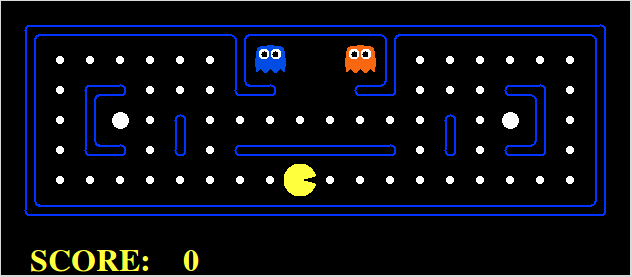
\includegraphics[width=120mm]{images/pacman_small_map}
    \caption{Mapa pequeno do jogo Pacman. Usado nos testes 1 e 3.}
    \label{img:PlataformaPacmanMapaPequeno}
\end{figure}

\subsubsection{Parâmetros Utilizados}

\begin{multicols}{2}

Num. partidas%
\footnote{Número de partidas executadas%
} = 3000;

Num. treinos%
\footnote{Número de partidas usadas para treinamento%
} = 2700;

Num. Greedy%
\footnote{Número de partidas em que foi utilizada exploração gulosa. Como explicado no tópico \ref{subsection:EscolhaDeAçõesExploraçãoGulosa}%
} = 1500;

$ \beta%
\footnote{Fator de exploração gulosa utilizado.%
} = 1 - \left( \frac{n}{Num. Greedy} \right) $;

$ \alpha%
\footnote{Fator de Aprendizagem%
} = 0.002 $;

$ \gamma%
\footnote{Fator de Desconto%
} = 0.99 $;

$ \sigma_{pacman}%
\footnote{Desvio padrão do erro gaussiano da posição recebida do Pacman%
} = 0.5 $;

$ \sigma_{dist\_fant}%
\footnote{Desvio padrão do erro gaussiano da distância recebida para os Fantasmas%
} = 0.5 $;

$ \nu_{atuacao}%
\footnote{Fator de Acerto na movimentação do Pacman. Descrito no algorítmo \ref{algorithm:ErroAtuacao} na seção \ref{section:AmbienteDeTestes}%
} = 0.9 $.

\end{multicols}

Sendo $ n $ o número da partida sendo jogada.

\subsubsection{Comportamentos Utilizados} \label{subsubsection:3ComportamentosUtilizados}

Os comportamentos utilizados foram: parar, comer e fugir. Ou seja:
$$ b \in B = \left\{ Ficar\_Parado, Comer, Fugir \right\}, $$
$$ s_b \in S_b = \left\{ Estado\_Parar, Estado\_Comer, Estado\_Fugir \right\}. $$

Como explicado no tópico \ref{subsection:BayesComSelecaoDeComportamento} agora são usados três modelos de seleção de ação motora: 

\begin{equation}
    P \left( M^t \mid S^t S_b^t M^{t-1} \pi_f \right) = 
        \left\{
            \begin{array}{l}
                P \left( M^t \mid S^t \left[ S_b^t=Estado\_Parar \right] M^{t-1} \pi \right) \\
                P \left( M^t \mid S^t \left[ S_b^t=Estado\_Comer \right] M^{t-1} \pi \right) \\
                P \left( M^t \mid S^t \left[ S_b^t=Estado\_Fugir \right] M^{t-1} \pi \right)
            \end{array}
        \right..
\end{equation}

A seguir, cada modelo é apresentado de forma detalhada.

\subsubsection*{Parar}

Esse é o comportamento mais simples, tendo como modelo de seleção de ação:

\begin{equation}
    P \left( m^t \mid S^t \left[ S_b^t = Estado\_Parar \right] M^{t-1} \pi_f \right) = 
        \left\{
            \begin{array}{l l}
                0.99 & \text{se }m^t = Parar \\
                0.0025 & \text{senão}
            \end{array}
        \right..
\end{equation}

\subsubsection*{Comer}

Para esse comportamento utiliza-se um modelo mais complexo em que, para um dado estado de $ S^t $ se calcula uma ação com o algoritmo \ref{algorithm:SelecaoDeAcaoComer}.

\begin{algorithm}[H]
	\caption{Escolher Ação Comer} \label{algorithm:SelecaoDeAcaoComer}
	\begin{algorithmic}[1]
		\Procedure{Escolher\_Ação\_Comer}{\textit{estado}}
			\State $\textit{pos\_comida} \gets \text{posição }\textit{comida\_mais\_proxima} $
			\State $\textit{pos\_pacman} \gets \text{posição }\textit{pacman} $
			\State $\textit{dist\_atual} \gets \text{dist} \left( \textit{pos\_comida}, \textit{pos\_pacman} \right) $
			\For{Ação $ in $ Ações}
				\State $\textit{nova\_pos\_pacman} \gets \text{executa} \left( \textit{pos\_pacman}, \textit{Ação} \right) $
				\If{$ \text{dist} \left( \textit{pos\_comida}, \textit{nova\_pos\_pacman} \right) < \textit{dist\_atual} $ }
					\State \Return $ \textit{Ação} $
					\Comment{Retorna ação escolhida}
				\EndIf 
			\EndFor
			\State \Return $ \textit{Ação} $
			\Comment{Nenhuma ação boa, mas precisa retornar uma}
		\EndProcedure
	\end{algorithmic}
\end{algorithm}

Depois de calculada essa ação para um estado $ s^t \in S^t $, utiliza-se um modelo parecido com o para o comportamento parado, apresentado na equação \ref{equation:ModeloAcaoComer}.

\begin{equation} \label{equation:ModeloAcaoComer}
    P \left( m^t \mid s^t \left[ S_b^t = Estado\_Comer \right] M^{t-1} \pi_f \right) = 
        \left\{
            \begin{array}{l l}
                0.99 & \text{se }m^t = \textit{Ação} \\
                0.0025 & \text{senão}
            \end{array}
        \right..
\end{equation}

\subsubsection*{Fugir}

Para esse comportamento é utilizado um formato parecido com o de comer, mas com uma escolha de ação diferente. Para um dado estado de $ S^t $ se calcula uma ação usando o algoritmo \ref{algorithm:SelecaoDeAcaoFugir}.

\begin{algorithm}[h]
	\caption{Escolher Ação Fugir} \label{algorithm:SelecaoDeAcaoFugir}
	\begin{algorithmic}[1]
		\Procedure{Escolher\_Ação\_Fugir}{\textit{estado}}
			\State $\textit{pos\_fantasma} \gets \text{posição }\textit{fantasma\_mais\_proximo} $
			\State $\textit{pos\_pacman} \gets \text{posição }\textit{pacman} $
			\State $\textit{dist\_atual} \gets \text{dist} \left( \textit{pos\_fantasma}, \textit{pos\_pacman} \right) $
			\For{Ação $ in $ Ações}
				\State $\textit{nova\_pos\_pacman} \gets \text{executa} \left( \textit{pos\_pacman}, \textit{Ação} \right) $
				\If{$ \text{dist} \left( \textit{pos\_fantasma}, \textit{nova\_pos\_pacman} \right) > \textit{dist\_atual} $ }
					\State \Return $ \textit{Ação} $
					\Comment{Retorna ação escolhida}
				\EndIf 
			\EndFor
			\State \Return $ \textit{Ação} $
			\Comment{Nenhuma ação boa, mas precisa retornar uma}
		\EndProcedure
	\end{algorithmic}
\end{algorithm}

Depois de calculado essa ação para um estado $ s^t \in S^t $, assim como para o comportamento anterior, utiliza-se um modelo parecido com o modelo utilizado pelo comportamento parado.

\begin{equation}
    P \left( m^t \mid s^t \left[ S_b^t = Estado\_Fugir \right] M^{t-1} \pi_f \right) = 
        \left\{
            \begin{array}{l l}
                0.99 & \text{se }m^t = \textit{Ação} \\
                0.0025 & \text{senão}
            \end{array}
        \right.
\end{equation}

\subsubsection{Vetor de Características Utilizado} \label{subsubsection:3ComportamentosVetorCaracterísticas}

\subsubsection*{Bias}

Essa é uma característica que sempre está presente nesse vetor. Ela tem um valor padrão igual a $ 1.0 $ e seu peso $ \omega $ indica quão bom esse comportamento é, independente da situação atual.

$$ f_1 = 1.0 $$

\subsubsection*{Distância para Provável Comida mais Próxima} \label{subsubsection:DistProvavelComida}

Essa característica é proporcional à distância até a posição mais próxima em que é provável existir uma comida. Ela pode ser obtida a partir do algoritmo \ref{algorithm:ObterCaracteristicaDistanciaComida}.

\begin{algorithm}[H]
	\caption{Obter Característica Distancia Comida} \label{algorithm:ObterCaracteristicaDistanciaComida}
	\begin{algorithmic}[1]
		\Procedure{ObterCaracterísticaDistanciaComida}{\textit{probabilidades\_estados}}
			\State $\textit{max\_prob} \gets 0.0 $
			\For{Posição $ in $ Posições}
				\State $\textit{prob\_comida} \gets \text{probabilidade de comida } \left( \textit{Posição} \right) $
				\If{ $ \textit{prob\_comida} > \textit{max\_prob} $ }
					\State $\textit{max\_prob} \gets \textit{prob\_comida} $
				\EndIf 
			\EndFor
			\For{Posição $ in $ Posições}
				\State $\textit{prob\_comida} \gets \text{probabilidade de comida } \left( \textit{Posição} \right) $
				\If{ $ \textit{prob\_comida} > \frac{\textit{max\_prob} }{2} $ }
					\State $ \text{Prob\_Posições } append \text{ Posição} $
				\EndIf 
			\EndFor
			\State $\textit{pos\_comida} \gets \text{mais proxima }\textit{posição} \in \text{Prob\_Posições} $
			\State $\textit{pos\_pacman} \gets \text{posição }\textit{pacman} $
			\State \Return $ \text{dist} \left( \textit{pos\_comida}, \textit{pos\_pacman} \right)  $
		\EndProcedure
	\end{algorithmic}
\end{algorithm}

Tendo um conjunto de probabilidades $ a \in A $ para os estados:

$$ f_2 = \frac{ObterCaracteristicaDistanciaComida \left( a \right)}{\textit{área\_mapa}} $$

\subsubsection*{Soma das Probabilidades de Fantasmas a menos de 4 Movimentos}

Essa característica é obtida a partir da soma das probabilidades de haver fantasmas a 3 movimentos de distância, ou menos, podendo então ter valor no intervalo $ \left[ 0, num\_fantasmas \cdot 100\% \right] $. O valor dessa característica é obtida utilizando o algorítmo \ref{algorithm:ObterCaracteristicaProbabilidadesFantasmas}.

\begin{algorithm}[H]
	\caption{Obter Característica Probabilidades Fantasmas} \label{algorithm:ObterCaracteristicaProbabilidadesFantasmas}
	\begin{algorithmic}[1]
		\Procedure{ObterCaracterísticaProbFantasmas}{\textit{probabilidades\_estados}}
			\State $\textit{total} \gets 0.0 $
			\For{Posição $ in $ Posições}
				\For{Posição2 $ in $ Posições}
					\If{ $ \text{dist} \left( \textit{Posição} , \textit{Posição2} \right) < 4 $ }
						\State $\textit{prob\_pacman} \gets \text{probabilidade pacman } \left( \textit{Posição} \right) $
						\For{Fantasma $ in $ Fantasmas}
							\State $\textit{prob\_fantasma} \gets \text{probabilidade Fantasma } \left( \textit{Posição2} \right) $
							\State $\textit{prob\_normal} \gets \text{probabilidade estar normal } \left( \textit{Fantasma} \right) $
							\Comment{Não branco}
							\State $\textit{total} \gets \textit{total} + \textit{prob\_pacman}  \cdot \textit{prob\_fantasma} \cdot \textit{prob\_normal} $
						\EndFor
					\EndIf
				\EndFor
			\EndFor
			\State \Return $ \textit{total} $
		\EndProcedure
	\end{algorithmic}
\end{algorithm}

$$ f_3 = ObterCaracteristicaProbFantasmas \left( a \right) $$


\subsection{3 Comportamentos no mapa original (Teste 2)} \label{subsection:3ComportamentosMapaOriginal}

Esse teste é realizado no mapa clássico do jogo, mostrado na figura \ref{img:PlataformaPacmanMapaClássico}, e nele são utilizados apenas três comportamentos:

\begin{itemize}
	\item Parar;
	\item Comer;
	\item Fugir.
\end{itemize}

\begin{figure}[h]
    \centering
    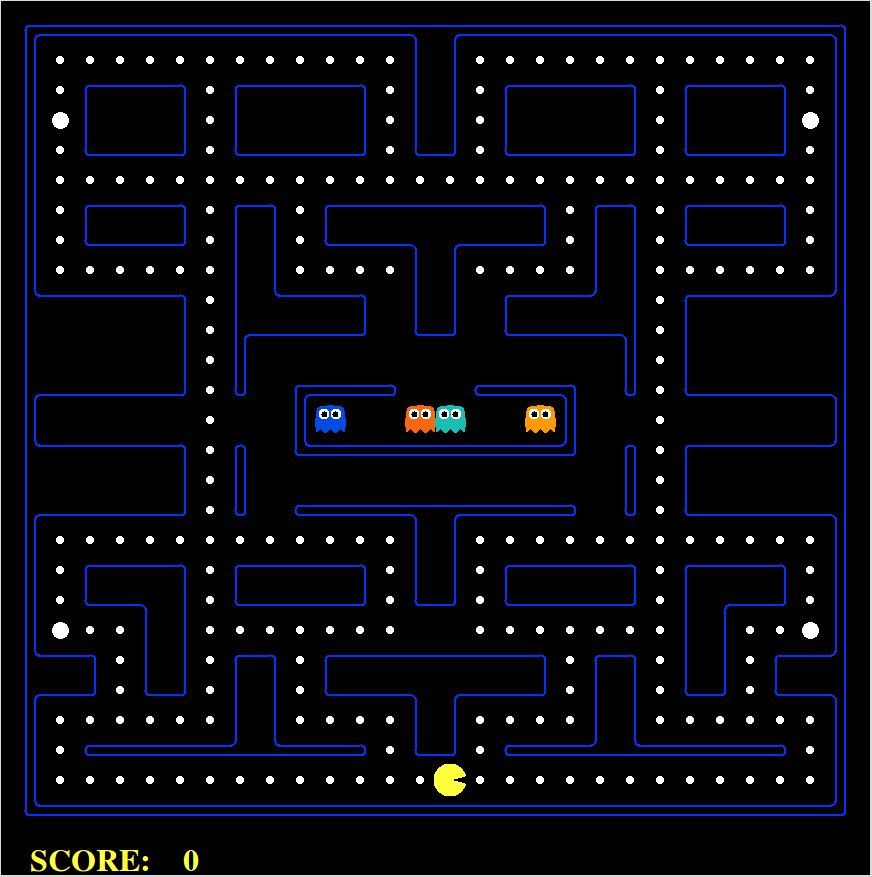
\includegraphics[width=120mm]{images/pacman_classical_map}
    \caption{Mapa clássico do jogo Pacman. Usado nos testes 2 e 4.}
    \label{img:PlataformaPacmanMapaClássico}
\end{figure}

\subsubsection{Parâmetros Utilizados}

\begin{multicols}{2}

Num. partidas = 1000;

Num. treinos = 700;

Num. Greedy = 500;

$ \beta = 1 - \left( \frac{n}{Num. Greedy} \right) $;

$ \alpha = 0.001 $;

$ \gamma = 0.99 $;

$ \sigma_{pacman} = 0.5 $;

$ \sigma_{dist\_fant} = 0.5 $;

$ \nu_{atuacao} = 0.9 $.

\end{multicols}

Sendo $ n $ o número da partida sendo jogada.

\subsubsection{Comportamentos Utilizados}

Os comportamentos utilizados foram os mesmos que para o teste anterior e estão descritos no tópico \ref{subsubsection:3ComportamentosUtilizados}.

\subsubsection{Vetor de Características Utilizado}

Para o vetor de características $ f $, são utilizados parâmetros semelhantes aos do teste anterior, sendo o único diferente o uso da $ \textit{Proximidade para Provável Comida mais Próxima} $ no lugar da $ \textit{Distância para Provável Comida mais Próxima} $.

\subsubsection*{Bias}

$$ f_1 = 1.0 $$

\subsubsection*{Proximidade para Provável Comida mais Próxima}

Essa é a única característica alterada do teste anterior para esse. Essa proximidade é utilizada, no lugar da distância, por ter um valor mais alto quando recompensas são recebidas e mais baixo no caso contrário, o que facilita a aprendizagem. Isso pode ser observado na equação \ref{equation:UpdateOmegaQPartiallyObservable}, com um valor $ f_i \left( a, b \right) $ maior, para um mesmo $ erro $, tem-se uma variação maior de $ \omega_i $ ($ \uparrow f_i \rightarrow \uparrow \Delta \omega_i $).

$$ f_2 = \frac{1}{ObterCaracteristicaDistanciaComida \left( a \right) } $$

\subsubsection*{Soma das Probabilidades de Fantasmas a menos de 4 Movimentos}

$$ f_3 = ObterCaracteristicaProbFantasmas \left( a \right) $$

\subsection{5 Comportamentos no mapa pequeno (Teste 3)} \label{subsection:5ComportamentosMapaPequeno}

Esse teste é feito no mapa pequeno, mostrado na figura \ref{img:PlataformaPacmanMapaPequeno}, e nele são utilizados todos os cinco comportamentos:

\begin{itemize}
	\item Parar;
	\item Comer;
	\item Fugir;
	\item Comer Cápsula;
	\item Caçar.
\end{itemize}

\subsubsection{Parâmetros Utilizados}

\begin{multicols}{2}

Num. partidas = 3000;

Num. treinos = 2700;

Num. Greedy = 1500;

$ \beta = 1 - \left( \frac{n}{Num. Greedy} \right) $;

$ \alpha = 0.002 $;

$ \gamma = 0.99 $;

$ \sigma_{pacman} = 0.5 $;

$ \sigma_{dist\_fant} = 0.5 $;

$ \nu_{atuacao} = 0.9 $.

\end{multicols}

Sendo $ n $ o número da partida sendo jogada.


\subsubsection{Comportamentos Utilizados} \label{subsubsection:5ComportamentosUtilizados}

Os comportamentos utilizados são: parar, comer, fugir, comer cápsula e caçar. Ou seja:
$$ b \in B = \left\{ Ficar\_Parado, Comer, Fugir, \textit{Comer\_Cápsula}, \textit{Caçar} \right\} $$
$$ s_b \in S_b = 
        \left\{
            \begin{array}{l}
                Estado\_Parar, \\
                Estado\_Comer, \\
                Estado\_Fugir, \\
                \textit{Estado\_Comer\_Cápsula}, \\
                \textit{Estado\_Caçar}
            \end{array}
        \right\}
         $$

Como explicado no tópico \ref{subsection:BayesComSelecaoDeComportamento}, e analogamente ao visto para três comportamentos, agora se tem cinco modelos de seleção de ação motora:
\begin{equation}
    P \left( M^t \mid S^t S_b^t M^{t-1} \pi_f \right) = 
        \left\{
            \begin{array}{l}
                P \left( M^t \mid S^t \left[ S_b^t=Estado\_Parar \right] M^{t-1} \pi \right) \\
                P \left( M^t \mid S^t \left[ S_b^t=Estado\_Comer \right] M^{t-1} \pi \right) \\
                P \left( M^t \mid S^t \left[ S_b^t=Estado\_Fugir \right] M^{t-1} \pi \right) \\
                P \left( M^t \mid S^t \left[ S_b^t=\textit{Estado\_Comer\_Cápsula} \right] M^{t-1} \pi \right) \\
                P \left( M^t \mid S^t \left[ S_b^t=\textit{Estado\_Caçar} \right] M^{t-1} \pi \right)
            \end{array}
        \right.
\end{equation}

Os modelos para os estados $ Estado\_Parar $, $ Estado\_Comer $ e $ Estado\_Fugir $ foram os mesmo utilizados no primeiro experimento e estão descritos no tópico \ref{subsubsection:3ComportamentosUtilizados}. Os outros dois modelos, para os estados de comportamento $ \textit{Estado\_Comer\_Cápsula} $ e $ \textit{Estado\_Caçar} $, estão descritos a seguir.

\subsubsection*{Comer Cápsula}

O modelo para o estado $ \textit{Estado\_Comer\_Cápsula} $ é análogo ao do estado $ Estado\_Comer $. Para um dado estado $ s^t \in S^t $ se calcula uma ação utilizando o algoritmo \ref{algorithm:SelecaoDeAcaoComerCápsula}.

\begin{algorithm}[H]
	\caption{Escolher Ação Comer Cápsula} \label{algorithm:SelecaoDeAcaoComerCápsula}
	\begin{algorithmic}[1]
		\Procedure{EscolherAçãoComerCápsula}{\textit{estado}}
			\State $\textit{pos\_capsula} \gets \text{posição }\textit{capsula\_mais\_proxima} $
			\State $\textit{pos\_pacman} \gets \text{posição }\textit{pacman} $
			\State $\textit{dist\_atual} \gets \text{dist} \left( \textit{pos\_comida}, \textit{pos\_pacman} \right) $
			\For{Ação $ in $ Ações}
				\State $\textit{nova\_pos\_pacman} \gets \text{executa} \left( \textit{pos\_pacman}, \textit{Ação} \right) $
				\If{$ \text{dist} \left( \textit{pos\_capsula}, \textit{nova\_pos\_pacman} \right) < \textit{dist\_atual} $ }
					\State \Return $ \textit{Ação} $
					\Comment{Retorna ação escolhida}
				\EndIf 
			\EndFor
			\State \Return $ \textit{Ação} $
			\Comment{Nenhuma ação boa, mas precisa retornar uma}
		\EndProcedure
	\end{algorithmic}
\end{algorithm}

Depois de calculada essa ação para um estado $ s^t \in S^t $, o modelo probabilístico da equação \ref{equation:PegarAcaoComerCapsula} é utilizado.

\begin{equation} \label{equation:PegarAcaoComerCapsula}
    P \left( m^t \mid s^t \left[ S_b^t = \textit{Estado\_Comer\_Cápsula} \right] M^{t-1} \pi_f \right) = 
        \left\{
            \begin{array}{l l}
                0.99 & \text{se }m^t = \textit{Ação} \\
                0.0025 & \text{senão}
            \end{array}
        \right..
\end{equation}


\subsubsection*{Caçar}

O modelo para o estado $ \textit{Estado\_Caçar} $ é análogo ao do estado $ Estado\_Fugir $, exceto por ir em direção ao fantasma e não para longe dele. Para um dado estado $ s^t \in S^t $ se calcula uma ação com o seguinte algoritmo:

\begin{algorithm}[H]
	\caption{Escolher Ação Caçar} \label{algorithm:SelecaoDeAcaoCaçar}
	\begin{algorithmic}[1]
		\Procedure{EscolherAçãoCaçar}{\textit{estado}}
			\State $\textit{pos\_fantasma} \gets \text{posição }\textit{fantasma\_mais\_proximo} $
			\State $\textit{pos\_pacman} \gets \text{posição }\textit{pacman} $
			\State $\textit{dist\_atual} \gets \text{dist} \left( \textit{pos\_fantasma}, \textit{pos\_pacman} \right) $
			\For{Ação $ in $ Ações}
				\State $\textit{nova\_pos\_pacman} \gets \text{executa} \left( \textit{pos\_pacman}, \textit{Ação} \right) $
				\If{$ \text{dist} \left( \textit{pos\_fantasma}, \textit{nova\_pos\_pacman} \right) < \textit{dist\_atual} $ }
					\State \Return $ \textit{Ação} $
					\Comment{Retorna ação escolhida}
				\EndIf 
			\EndFor
			\State \Return $ \textit{Ação} $
			\Comment{Nenhuma ação boa, mas precisa retornar uma}
		\EndProcedure
	\end{algorithmic}
\end{algorithm}

Uma vez calculada a ação para um estado $ s^t \in S^t $, utiliza-se o seguinte modelo probabilístico:

\begin{equation}
    P \left( m^t \mid s^t \left[ S_b^t = \textit{Estado\_Caçar} \right] M^{t-1} \pi_f \right) = 
        \left\{
            \begin{array}{l l}
                0.99 & \text{se }m^t = \textit{Ação} \\
                0.0025 & \text{senão}
            \end{array}
        \right..
\end{equation}

\subsubsection{Vetor de Características Utilizado} \label{subsubsection:5ComportamentosVetorCaracterísticas}

O vetor de características $ f $ para esse experimento tem sete parâmetros, sendo 3 deles os usados no experimento anterior (\ref{subsection:3ComportamentosMapaOriginal}) $ Bias $, \textit{Proximidade para Provável Comida mais Próxima} e \textit{Soma das Probabilidades de Fantasmas a menos de 4 Movimentos}. Os outros quatro são:

\begin{itemize}
	\item \textit{Proximidade para Provável Cápsula mais Próxima};
	\item \textit{Probabilidade de ainda Existir uma Cápsula};
	\item \textit{Probabilidade de Existir Fantasma Branco};
	\item \textit{Soma das Probabilidades de Fantasmas Brancos a menos de 4 Movimentos}.
\end{itemize}

Cada uma dessas características está descrita a seguir.

\subsubsection*{Bias}
$$ f_1 = 1.0 $$

\subsubsection*{Proximidade para Provável Comida mais Próxima}
$$ f_2 = \frac{1}{ObterCaracteristicaDistanciaComida \left( a \right)} $$

\subsubsection*{Proximidade para Provável Cápsula mais Próxima}

Essa característica indica qual a proximidade até a posição mais próxima em que é provável existir uma cápsula. Ela pode ser obtida a partir do algoritmo \ref{algorithm:ObterCaracteristicaDistanciaCapsula}, que é análogo ao algoritmo \ref{algorithm:ObterCaracteristicaDistanciaComida} do tópico \ref{subsubsection:DistProvavelComida}.

\begin{algorithm}[H]
	\caption{Obter Característica Distancia Cápsula} \label{algorithm:ObterCaracteristicaDistanciaCapsula}
	\begin{algorithmic}[1]
		\Procedure{ObterCaracterísticaDistanciaCápsula}{\textit{probabilidades\_estados}}
			\State $\textit{max\_prob} \gets 0.0 $
			\For{Posição $ in $ Posições}
				\State $\textit{prob\_capsula} \gets \text{probabilidade de capsula } \left( \textit{Posição} \right) $
				\If{ $ \textit{prob\_capsula} > \textit{max\_prob} $ }
					\State $\textit{max\_prob} \gets \textit{prob\_capsula} $
				\EndIf 
			\EndFor
			\For{Posição $ in $ Posições}
				\State $\textit{prob\_capsula} \gets \text{probabilidade de capsula } \left( \textit{Posição} \right) $
				\If{ $ \textit{prob\_capsula} > \frac{\textit{max\_prob} }{2} $ }
					\State $ \text{Prob\_Posições } append \text{ Posição} $
				\EndIf 
			\EndFor
			\State $\textit{pos\_capsula} \gets \text{mais proxima }\textit{posição} \in \text{Prob\_Posições} $
			\State $\textit{pos\_pacman} \gets \text{posição }\textit{pacman} $
			\State \Return $ \text{dist} \left( \textit{pos\_capsula}, \textit{pos\_pacman} \right) $
		\EndProcedure
	\end{algorithmic}
\end{algorithm}

Tendo um conjunto de probabilidades $ a \in A $ para os estados:

$$ f_3 = \frac{1}{ObterCaracteristicaDistanciaCapsula \left( a \right)} $$

\subsubsection*{Probabilidade de ainda Existir uma Cápsula}

Essa característica é obtida a partir da probabilidade de ainda existir uma cápsula no mapa.

$$ f_4 = P \left( capsula \mid a \right) $$

\subsubsection*{Probabilidade de Existir Fantasma Branco}

Essa característica é obtida a partir da probabilidade de existir um fantasma branco no ambiente.

$$ f_5 = P \left( fantasma\_branco \mid a \right) $$

\subsubsection*{Soma das Probabilidades de Fantasmas a menos de 4 Movimentos}

$$ f_6 = ObterCaracteristicaProbFantasmas \left( a \right) $$

\subsubsection*{Soma das Probabilidades de Fantasmas Brancos a menos de 4 Movimentos}

Essa característica é obtida a partir da soma das probabilidades de haver fantasmas a 3 movimentos de distância, ou menos, podendo então ter valor entre $ \left[ 0, num\_fantasmas \cdot 100\% \right] $. Ela pode ser obtida a partir do algorítmo \ref{algorithm:ObterCaracteristicaProbabilidadesFantasmasBrancos}.

\begin{algorithm}[H]
	\caption{Obter Característica Probabilidades Fantasmas Brancos} \label{algorithm:ObterCaracteristicaProbabilidadesFantasmasBrancos}
	\begin{algorithmic}[1]
		\Procedure{ObterCaracterísticaProbFantasmasBrancos}{\textit{probabilidades\_estados}}
			\State $\textit{total} \gets 0.0 $
			\For{Posição $ in $ Posições}
				\For{Posição2 $ in $ Posições}
					\If{ $ \text{dist} \left( \textit{Posição} , \textit{Posição2} \right) < 4 $ }
						\State $\textit{prob\_pacman} \gets \text{probabilidade pacman } \left( \textit{Posição} \right) $
						\For{Fantasma $ in $ Fantasmas}
							\State $\textit{prob\_fantasma} \gets \text{probabilidade Fantasma } \left( \textit{Posição2} \right) $
							\State $\textit{prob\_branco} \gets \text{probabilidade estar branco } \left( \textit{Fantasma} \right) $
							\State $\textit{total} \gets \textit{total} + \textit{prob\_pacman}  \cdot \textit{prob\_fantasma} \cdot \textit{prob\_branco} $
						\EndFor
					\EndIf
				\EndFor
			\EndFor
			\State \Return $ \textit{total} $
		\EndProcedure
	\end{algorithmic}
\end{algorithm}

$$ f_7 = ObterCaracteristicaProbFantasmasBrancos \left( a \right) $$

\subsection{5 Comportamentos no mapa original (Teste 4)} \label{subsection:5ComportamentosMapaOriginal}

Esse teste é feito no mapa clássico do jogo, apresentado na figura \ref{img:PlataformaPacmanMapaClássico}, e nele, como no teste anterior (tópico \ref{subsection:5ComportamentosMapaPequeno}), são utilizados todos os cinco comportamentos:

\begin{itemize}
	\item Parar;
	\item Comer;
	\item Fugir;
	\item Comer Cápsula;
	\item Caçar.
\end{itemize}

\subsubsection{Parâmetros Utilizados}

\begin{multicols}{2}

Num. partidas = 1000;

Num. treinos = 700;

Num. Greedy = 500;

$ \beta = 1 - \left( \frac{n}{Num. Greedy} \right) $;

$ \alpha = 0.001 $;

$ \gamma = 0.99 $;

$ \sigma_{pacman} = 0.5 $;

$ \sigma_{dist\_fant} = 0.5 $;

$ \nu_{atuacao} = 0.9 $.

\end{multicols}

Sendo $ n $ o número da partida sendo jogada.


\subsubsection{Comportamentos Utilizados}

Os comportamentos utilizados são os mesmos do experimento anterior (\ref{subsection:5ComportamentosMapaPequeno}), descritos no tópico \ref{subsubsection:5ComportamentosUtilizados}.

\subsubsection{Vetor de Características Utilizado}

O vetor de características $ f $ usado nesse experimento possui seis características, sendo cinco delas iguais às utilizadas no experimento anterior%
\footnote{Essas características estão melhor descritos no tópico \ref{subsubsection:5ComportamentosVetorCaracterísticas}.%
}. A última é uma combinação das duas restantes: \textit{Proximidade para Provável Capsula mais Próxima} e \textit{Probabilidade de ainda Existir uma Capsula}.  O vetor possui, então, as seguintes características:

\subsubsection*{Bias}
$$ f_1 = 1.0 $$

\subsubsection*{Proximidade para Provável Comida mais Próxima}
$$ f_2 = \frac{1}{ObterCaracteristicaDistanciaComida \left( a \right)} $$

\subsubsection*{Probabilidade e Proximidade para Provável Cápsula mais Próxima }

Essa é a característica nova inserida para esse experimento e simplifica as duas características anteriores \textit{Proximidade para Provável Capsula mais Próxima} e \textit{Probabilidade de ainda Existir uma Capsula}, sendo o produto das duas.
$$ f_3 = \frac{P \left( capsula \mid a \right)}{ObterCaracteristicaDistanciaCapsula \left( a \right)} $$

\subsubsection*{Probabilidade de Existir Fantasma Branco}
$$ f_4 = P \left( fantasma\_branco \mid a \right) $$

\subsubsection*{Soma das Probabilidades de Fantasmas a menos de 4 Movimentos}
$$ f_5 = ObterCaracteristicaProbFantasmas \left( a \right) $$

\subsubsection*{Soma das Probabilidades de Fantasmas Brancos a menos de 4 Movimentos}
$$ f_6 = ObterCaracteristicaProbFantasmasBrancos \left( a \right) $$





\begin{comment}
Resultados
\end{comment}
%TCIDATA{LaTeXparent=0,0,relatorio.tex}



\chapter{Análise de Dados} \label{chap:Resultados}

% Resumo opcional. Comentar se não usar.
\resumodocapitulo{``Analisar os dados tops!'' -- Tiago}


\section{Introdução}

Nesse capítulo iremos explicar um pouco melhor os experimentos realizados, descritos na seção \ref{section:TestesRealizados}. Iremos também mostrar seus resultados e analisá-los. Lembrando que os experimentos realizados foram:

\begin{itemize}
	\item Apendizagem de 3 comportamentos em um mapa pequeno
	\item Apendizagem de 3 comportamentos no mapa clássico
	\item Apendizagem de 5 comportamentos em um mapa pequeno
	\item Apendizagem de 5 comportamentos no mapa clássico
\end{itemize}

\section{3 Comportamentos no mapa pequeno}

Nesse experimento%
\footnote{Os parâmetros e o setup desse experimento estão melhor descritos no tópico \ref{subsection:3ComportamentosMapaPequeno}.%
} utilizamos apenas 3 comportamentos, $ B = \{Ficar\_Parado, Comer, Fugir\} $, e usamos como vetor de características $ f $, sendo ele:

\begin{equation}
	\begin{array}{r l}
		Bias: & f_1 \left( a, u \right) = 1.0 \\
		Dist Comida: & f_2 \left( a, u \right) = ObterCaracteristicaDistanciaComida \left( a \right) \\
		Prob. Fantasma: & f_3 \left( a, u \right) = ObterCaracteristicaProbFantasmas \left( a \right)
	\end{array}
\end{equation}

Realizamos o treinamento ao longo de 2700 partidas, sendo que a exploração gulosa (\textit{greedy exploration}) foi executada até a partida 1500. Após terminado o treinamento utilizamos 300 partidas para avaliar e obter dados sobre o algoritmo treinado.


\subsection{Resultados e Análise}

A evolução da aprendizagem se dá a partir da mudança dos pesos $ \omega_i $ ao longo do tempo, devido à sua relação com o comportamento selecionado via a equaçào \ref{equation:QLearningEscolhaComportamentoFinal}. Nas figuras \ref{img:3ComportamentosMapaPequeno:PesoBias}, \ref{img:3ComportamentosMapaPequeno:PesoDistComida}, \ref{img:3ComportamentosMapaPequeno:PesoProbFantasma} temos os gráficos de como os valores desses pesos evoluem com o tempo, para cada um dos comportamentos.

\begin{figure}[H]
    \centering
    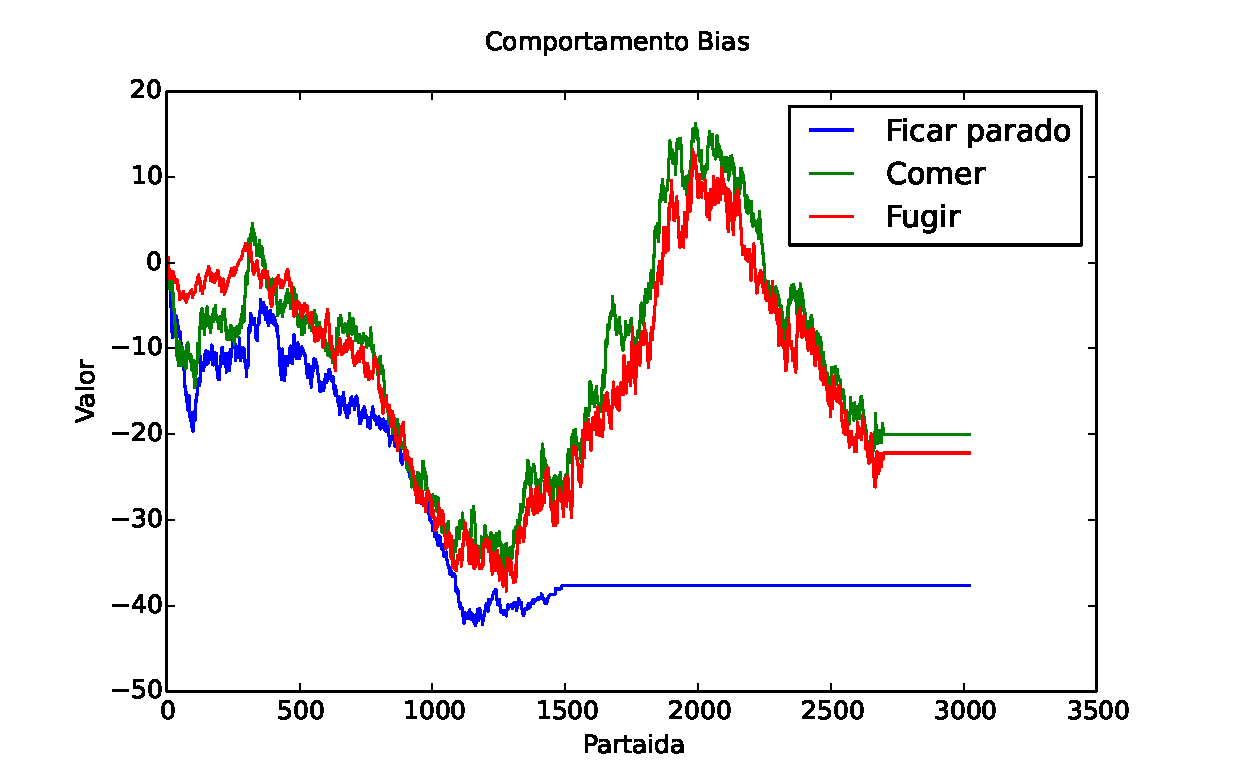
\includegraphics[width=\linewidth]{images/3_behaviors_small_map/weights____pol__Bias}
    \caption{Evolução dos pesos $ \omega_1 $ da característica Bias $ f_1 $.}
    \label{img:3ComportamentosMapaPequeno:PesoBias}
\end{figure}

\begin{figure}[H]
    \centering
    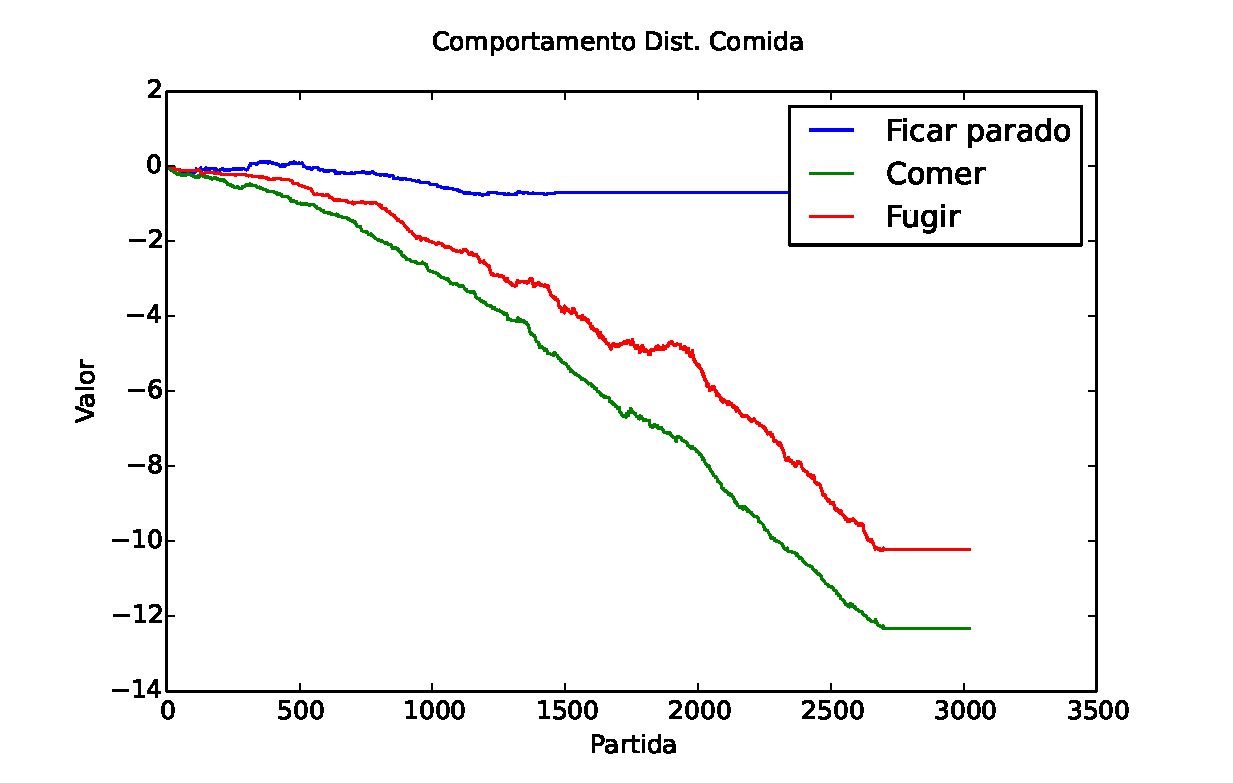
\includegraphics[width=\linewidth]{images/3_behaviors_small_map/weights____pol__DistComida}
    \caption{Evolução dos pesos $ \omega_2 $ da característica Distância para Comida $ f_2 $.}
    \label{img:3ComportamentosMapaPequeno:PesoDistComida}
\end{figure}

\begin{figure}[H]
    \centering
    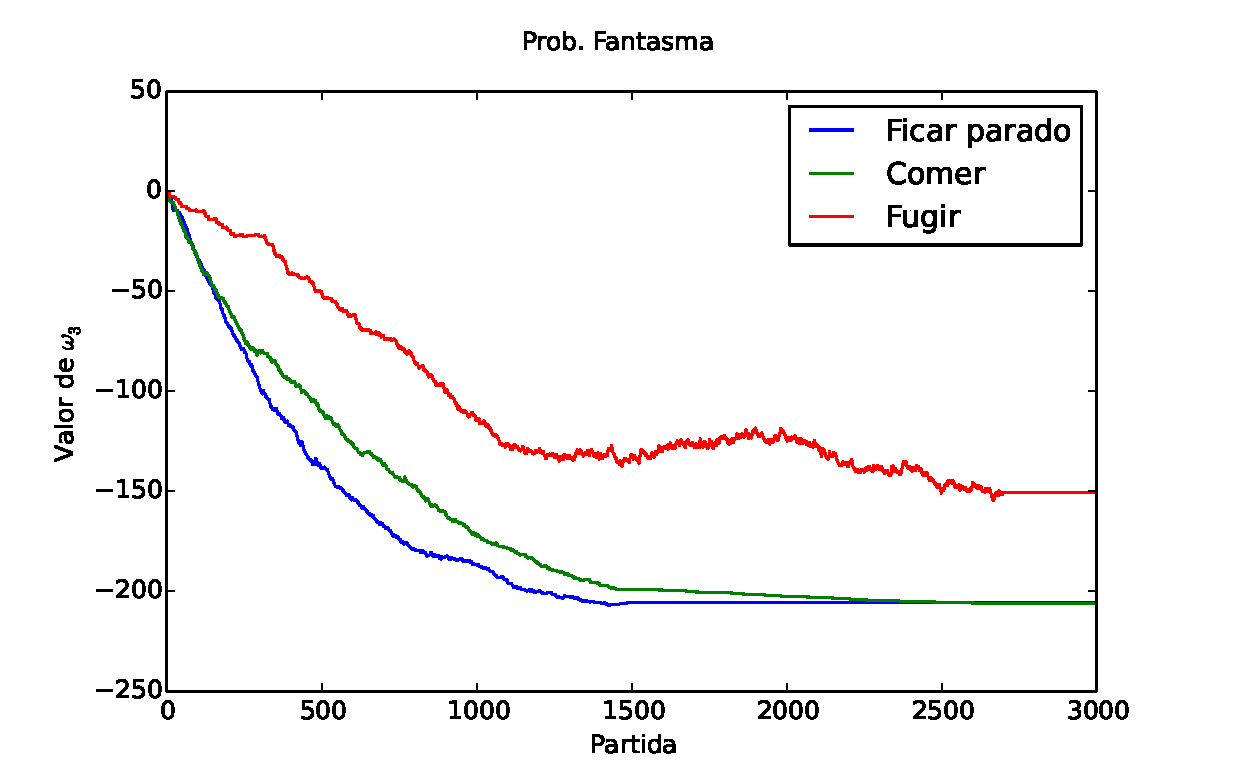
\includegraphics[width=\linewidth]{images/3_behaviors_small_map/weights____pol__ProbFantasma}
    \caption{Evolução dos pesos $ \omega_3 $ da característica Probabilidade de Fantasma $ f_3 $.}
    \label{img:3ComportamentosMapaPequeno:PesoProbFantasma}
\end{figure}

É fácil notar que o peso $ \omega_3 $, relativo à carascterística probabilidade de haver um fantasma normal perto, $ f_3 $, é o que cresce mais rápido e que atinge valor absoluto final maior, entre -140 e -210, enquanto os outros dois ficam entre -50 e 20. Isso acontece pois ele sempre tem um valor alto quando o pacman é morto, recebendo uma recompensa de -500 pontos. Quando os pesos são atualizados, seguindo as equações \ref{equation:ErroQPartiallyObservable} e \ref{equation:UpdateOmegaQPartiallyObservable}, esse peso será bastante modificado a cada morte do pacman. Isso mostra também que ele aprende que essa é uma situação ruim, dando um valor menor para estados em que ela tem valor mais alto ($ \uparrow f_3 \rightarrow \downarrow \downarrow Q $).

Outro fato ressaltado por esses gráficos é que estar perto de fantasmas é menos ruim no caso de se escolher o comportamento fugir, do que para comer ou ficar parado. Analisando esses valores é possível ver que o comportamento $ Ficar\_Parado $ nunca será executado%
\footnote{Lembrando que, como explicado no tópico \ref{subsection:3ComportamentosMapaPequeno}, o valor de $ f_2 \left( A, B \right) $ estará sempre entre 0 e 1.%
}, o comportamento $ Comer $ será o normalmente utilizado e o comportamento $ Fugir $ será utilizado quando a probabilidade de haver um fantasma por perto for alta.

Qual comportamento é escolhido a cada instante e quantas vezes cada um é escolhido por partida são fatores importantes para avaliar esse algoritmo. Quando pegamos o número de vezes que cada comportamentos é escolhido por partida e plotamos esses dados como pontos num gráfico eles formam a seguinte nuvem, exposta na figura \ref{img:3ComportamentosMapaPequeno:ComportamentosEscolhidos}.

\begin{figure}[H]
    \centering
    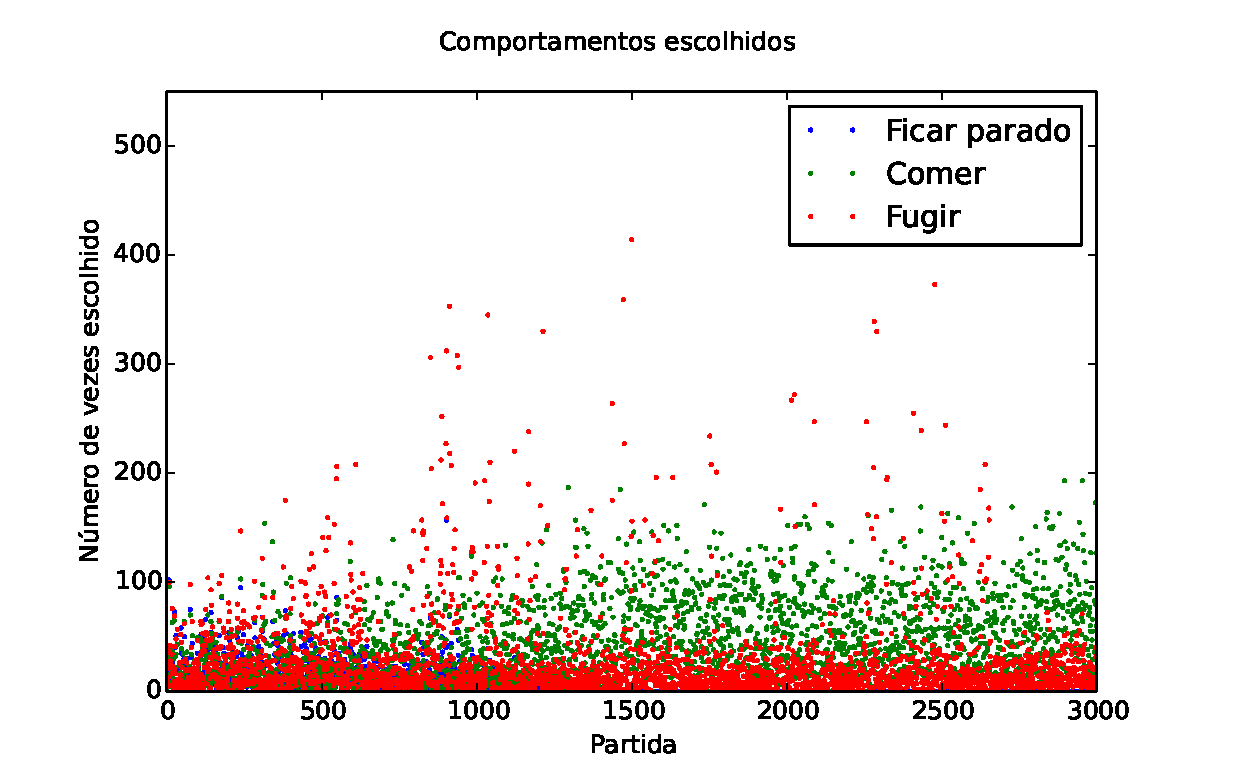
\includegraphics[width=\linewidth]{images/3_behaviors_small_map/chosen_behaviors}
    \caption{Escolha de comportamentos por partida.}
    \label{img:3ComportamentosMapaPequeno:ComportamentosEscolhidos}
\end{figure}

Com essa nuvem de dados já podemos começar a avaliar como essa escolha de comportamento é feita ao longo do tempo, mas para ter uma visualização melhor podemos aproximar um polinômio dessa nuvem de pontos, utilizando o método dos mínimos quadrados. Para um polinômio de quarto grau essa curva fica como a descrita na figura \ref{img:3ComportamentosMapaPequeno:ComportamentosEscolhidosPolinômio}.

\begin{figure}[H]
    \centering
    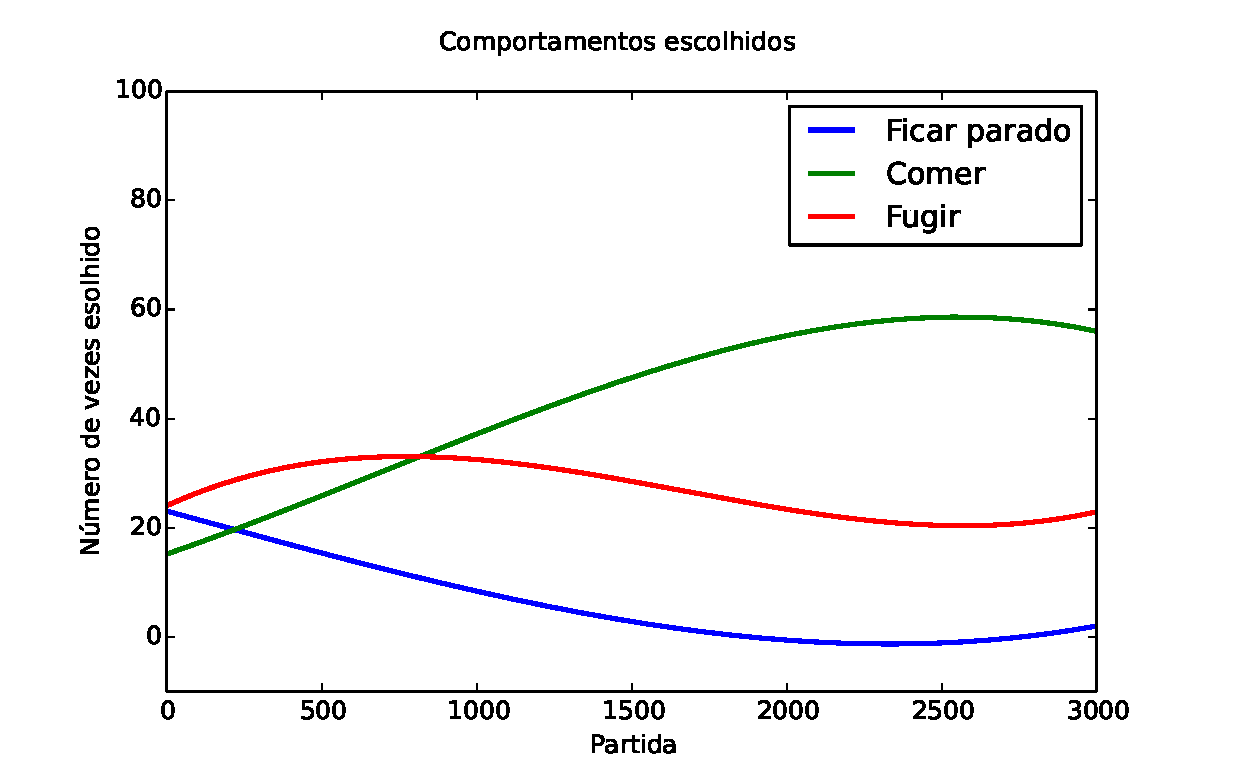
\includegraphics[width=\linewidth]{images/3_behaviors_small_map/chosen_behaviors_pol}
    \caption{Escolha de comportamentos por partida.}
    \label{img:3ComportamentosMapaPequeno:ComportamentosEscolhidosPolinômio}
\end{figure}

Inicialmente o comportamento $ Comer $ diminui em números de execução, enquanto $ Fugir $ aumenta. Isso acontece porque, inicialmente, não sabendo nada sobre o mundo, o agente ``percebe'' que quando ele executa o comportamento $ Comer $, ele tem muito mais probabilidade de morrer. Após aproximadamente 500 partidas, percebemos que esse comportamento começa a aumentar em número de execuções, enquanto o $ Fugir $ diminui.

Outro dado relevante para a análise é a pontuação obtida por jogo, que tentamos otimizar ao dá-la como recompensa para nossa função de treinamento. A pontuação para cada partida pode ser vista na imagem \ref{img:3ComportamentosMapaPequeno:PontuacaoPorPartida}, à seguir. Assim como para a evolução dos comportamentos escolhidos ao longo do tempo, também aproximamos esses dados por um polinômio, dessa vez de terceiro grau, utilizando o método dos mínimos quadrado.

\begin{figure}[H]
    \centering
    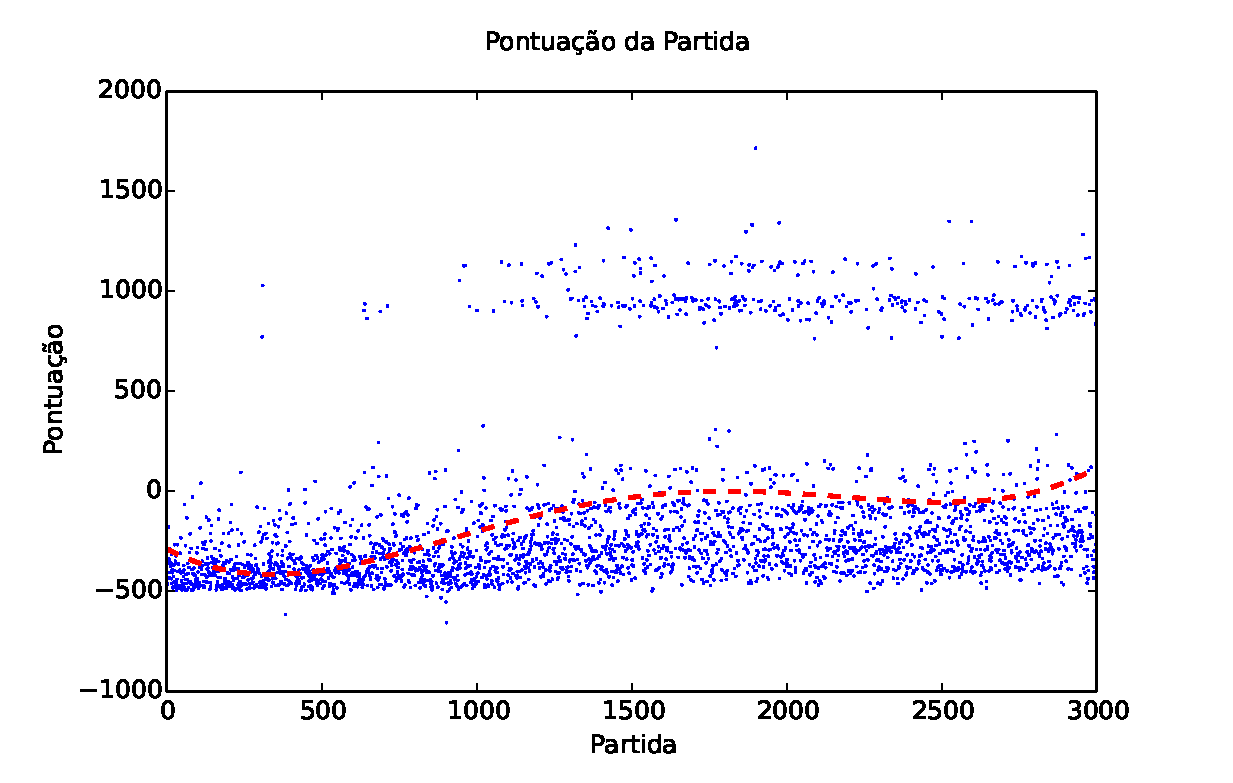
\includegraphics[width=\linewidth]{images/3_behaviors_small_map/match_scores____pol}
    \caption{Escolha de comportamentos por partida.}
    \label{img:3ComportamentosMapaPequeno:PontuacaoPorPartida}
\end{figure}

É possível perceber que essa função é ascendente e que segue, aproximadamente, o formato da curva do número de execuções do comportamento $ Comer $. Isso acontece pois, inicialmente, ao aumentar o número de execuções de $ Fugir $, se diminui a pontuação geral%
\footnote{Se não pegar uma comida, se perde um ponto por movimento.%
}. A média de pontos feita, após a conclusão do treinamento:

$$ mean \left( score \right) =50.04 $$

Sendo a média de escolha pelo algorítmo de aprendizagem dos comportamentos:

$$ mean \left( Ficar\_Parado \right) = 0.0 $$
$$ mean \left( Comer \right) = 61.77 $$
$$ mean \left( Fugir \right) = 17.21 $$


\subsection{Discussão}

Podemos ver que o algoritmo teve o resultado esperado para esse mapa e esses comportamentos, escolhendo sempre fugir, quando tendo alta probabilidade de perigo por perto, e comer no caso contrário.


\section{3 Comportamentos no mapa original (Teste 2)}

Nesse experimento%
\footnote{Os parâmetros e o setup desse experimento estão melhor descritos no tópico \ref{subsection:3ComportamentosMapaOriginal}.%
}, assim como no anterior, utilizamos apenas 3 comportamentos, $ B = \{Ficar\_Parado, Comer, Fugir\} $, e usamos como vetor de características $ f $, sendo ele:

\begin{equation}
	\begin{array}{r l}
		Bias: & f_1 \left( a, u \right) = 1.0 \\
		Dist Comida: & f_2 \left( a, u \right) = ObterCaracteristicaDistanciaComida \left( a \right) \\
		Prob. Fantasma: & f_3 \left( a, u \right) = ObterCaracteristicaProbFantasmas \left( a \right)
	\end{array}
\end{equation}

Realizamos o treinamento ao longo de 700 partidas, sendo que a exploração gulosa (\textit{greedy exploration}) foi executada até a partida 500. Após terminado o treinamento utilizamos 300 partidas para avaliar e obter dados sobre o algoritmo treinado.


\subsection{Resultados e Análise}

Como no experimento anterior, nas figuras à seguir \ref{img:3ComportamentosMapaOriginal:PesoBias}, \ref{img:3ComportamentosMapaOriginal:PesoDistComida}, \ref{img:3ComportamentosMapaOriginal:PesoProbFantasma} temos os gráficos de como os valores dos pesos $ \omega_i $ evoluem com o tempo, para cada um dos comportamentos.

\begin{figure}[H]
    \centering
    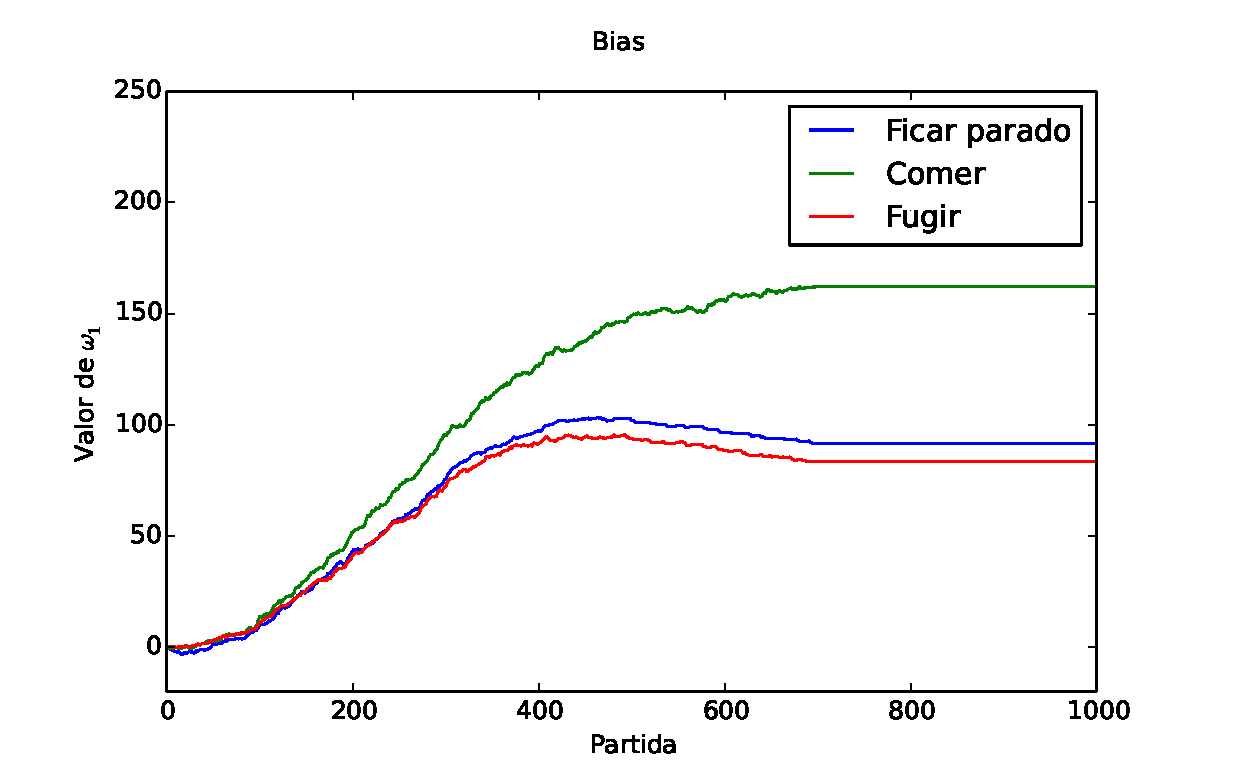
\includegraphics[width=\linewidth]{images/3_behaviors_original_map/weights____pol__Bias}
    \caption{Evolução dos pesos $ \omega_1 $ da característica Bias $ f_1 $.}
    \label{img:3ComportamentosMapaOriginal:PesoBias}
\end{figure}

\begin{figure}[H]
    \centering
    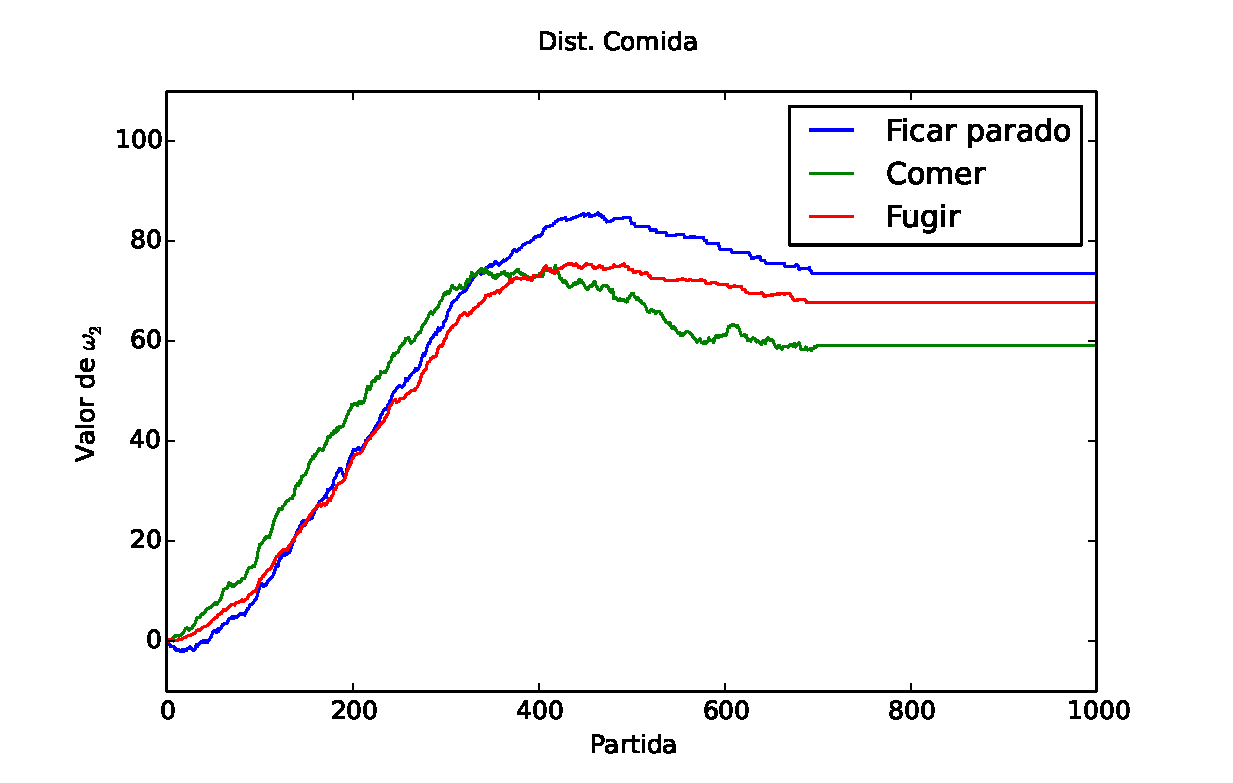
\includegraphics[width=\linewidth]{images/3_behaviors_original_map/weights____pol__DistComida}
    \caption{Evolução dos pesos $ \omega_2 $ da característica Distância para Comida $ f_2 $.}
    \label{img:3ComportamentosMapaOriginal:PesoDistComida}
\end{figure}

\begin{figure}[H]
    \centering
    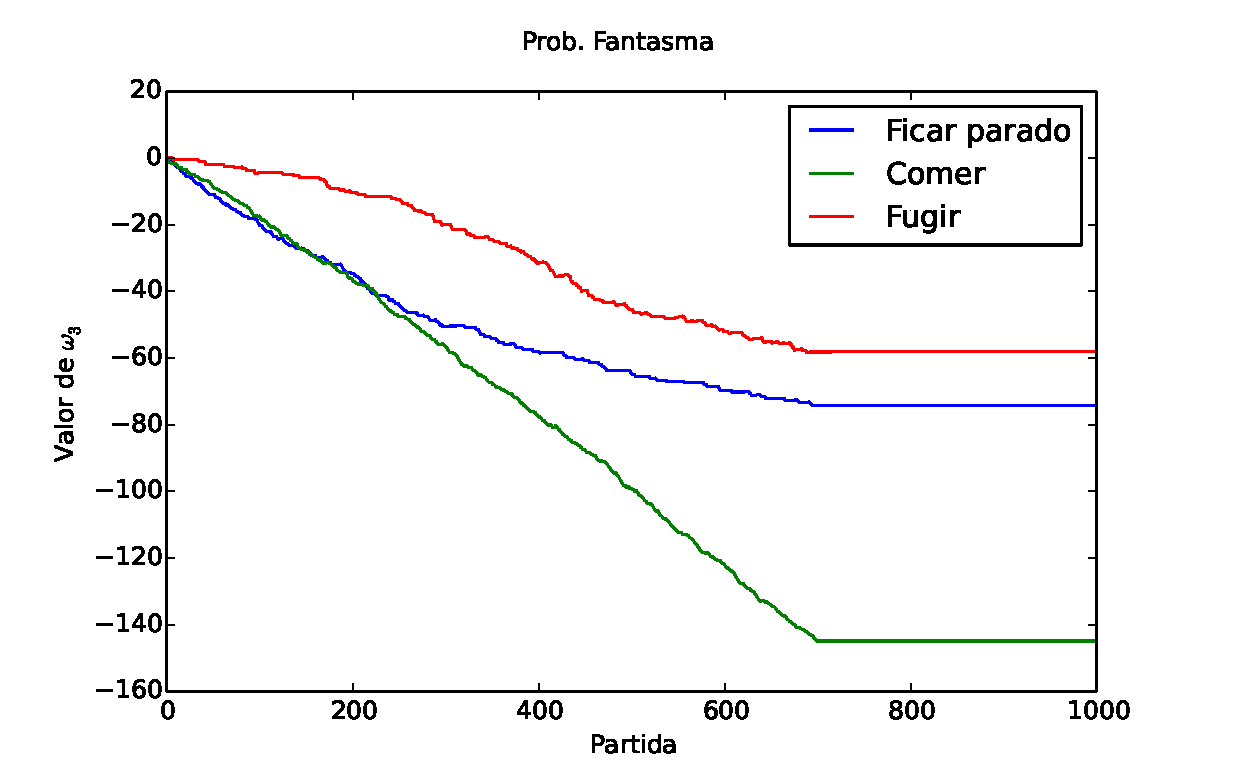
\includegraphics[width=\linewidth]{images/3_behaviors_original_map/weights____pol__ProbFantasma}
    \caption{Evolução dos pesos $ \omega_3 $ da característica Probabilidade de Fantasma $ f_3 $.}
    \label{img:3ComportamentosMapaOriginal:PesoProbFantasma}
\end{figure}

Podemos notar que, para esse experimento, todos os pesos, $ \omega_1 $, $ \omega_2 $ e $ \omega_3 $ , tem valores relativamente altos. Isso se dá, em boa parte, por esse ser um mapa ``fácil''. Como se demora mais para morrer, pois o mapa é grande e se tem menos chance de encontrar um fantasma, o peso da característica $ Prob. Fantasma $ cresce (ou diminui, já que é negativa) mais lentamente. Além disso, como se morre menos vezes, os pesos das outras características tende a aumentar mais do que diminuir.

Novamente, conseguimos reparar que o fato de $ \omega_3 $, o peso de $ Prob.Fantasma $, ser negativo e com valor absoluto alto para o comportamento $ Comer $, mostra que ele aprende que essa é uma situação ruim para se escolher esse comportamento. Também vemos novamente que estar perto de fantasmas é menos ruim no caso de se escolher o comportamento fugir, do que para comer ou ficar parado.

Um fato que pode parecer estranho a primeira vista é o fato de o peso $ \omega_2 $, da característica $ Dist. Comida $, ser maior para ficar parado e menor para comer. Isso ocorre pois os pesos devem se balancear pela equação de calculo do erro \ref{equation:ErroQPartiallyObservable} e, como $ Comer $ tem um peso $ \omega_1 $, da característica $ Bias $, alto, seus outros pesos acabam sendo afetados.

Analisando esses pesos vemos que o comportamento $ Comer $ será o normalmente utilizado, o comportamento $ Fugir $ será utilizado quando a probabilidade de haver um fantasma por perto for alta e o comportamento $ Ficar\_Parado $ será escolhido raramente, quando houver uma probabilidade mediana de haver um fantasma por perto e se estiver perto de uma comida.

Para esse experimento, quando plotamos o número de vezes que cada comportamentos é escolhido por partida como pontos num gráfico eles formam a nuvem exposta na figura \ref{img:3ComportamentosMapaOriginal:ComportamentosEscolhidos}.

\begin{figure}[H]
    \centering
    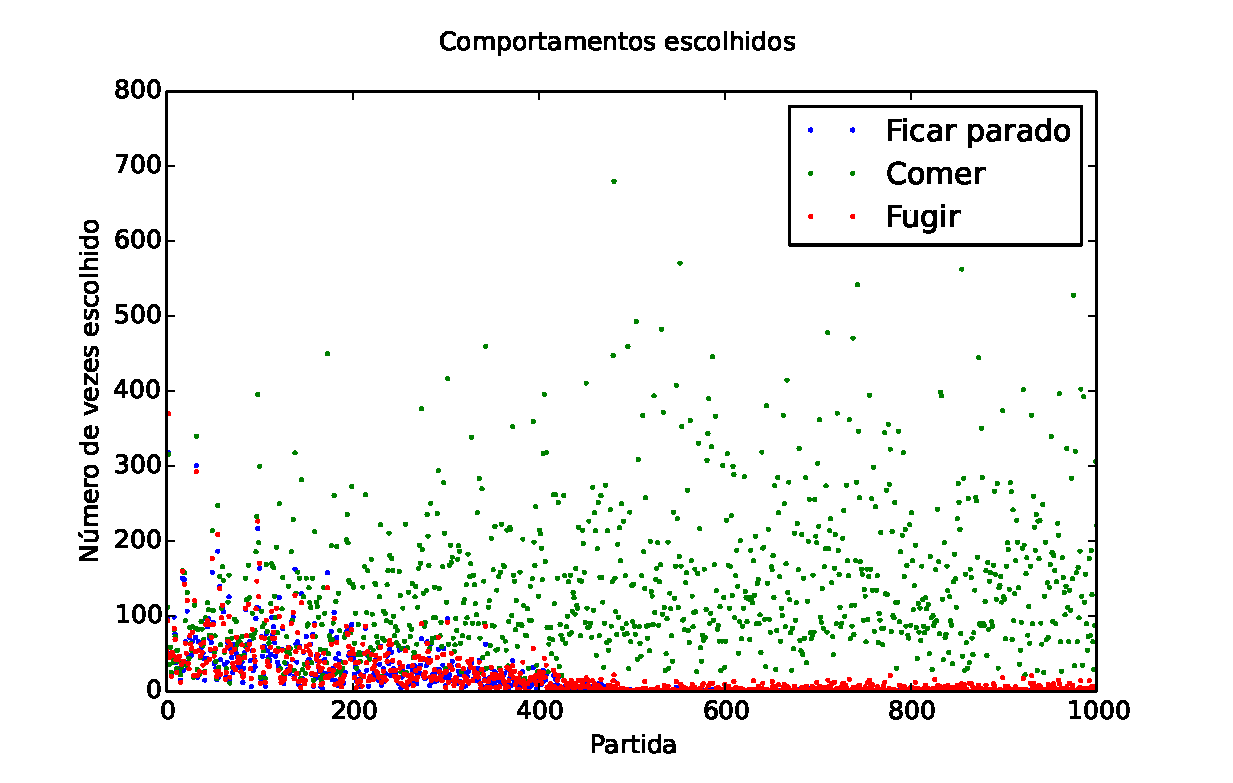
\includegraphics[width=\linewidth]{images/3_behaviors_original_map/chosen_behaviors}
    \caption{Escolha de comportamentos por partida.}
    \label{img:3ComportamentosMapaOriginal:ComportamentosEscolhidos}
\end{figure}

Novamente, para ter uma visualização melhor achamos um polinômio que represente essa nuvem de pontos, utilizando o método dos mínimos quadrados. Para um polinômio de quarto grau essa curva fica como a descrita na figura \ref{img:3ComportamentosMapaOriginal:ComportamentosEscolhidosPolinômio}.

\begin{figure}[H]
    \centering
    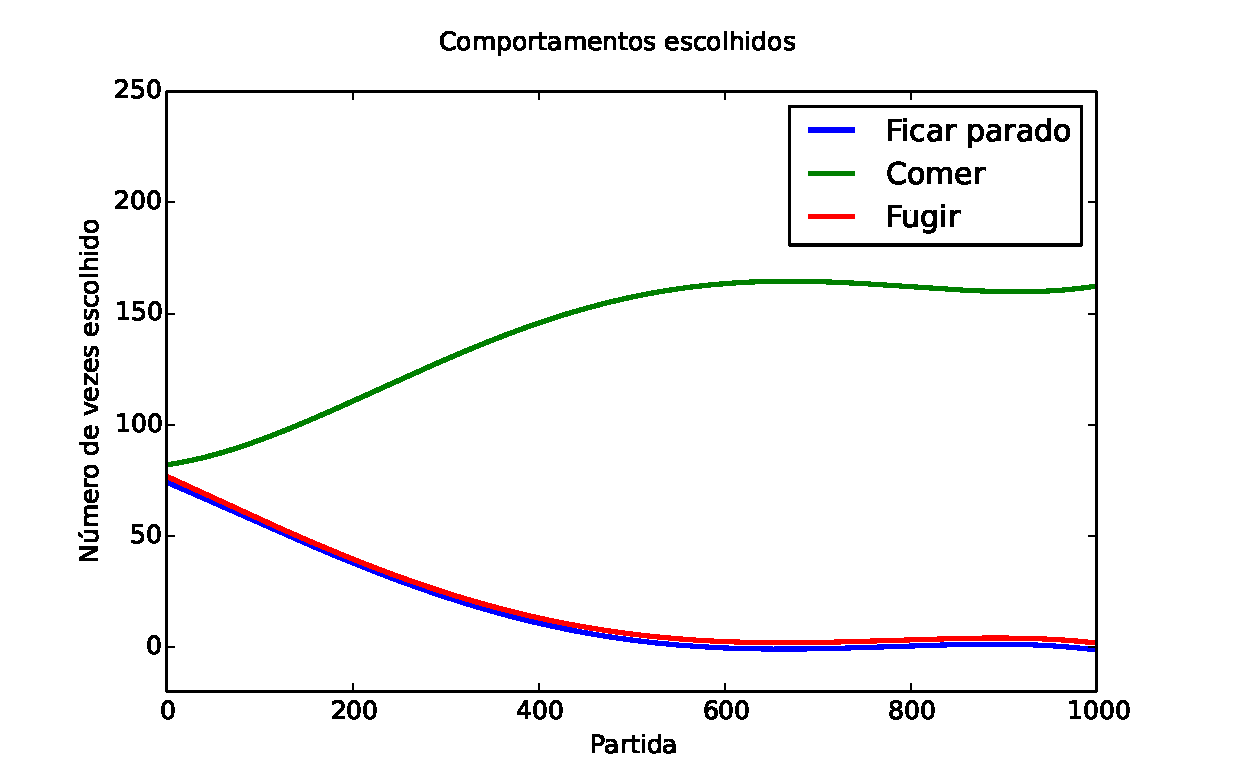
\includegraphics[width=\linewidth]{images/3_behaviors_original_map/chosen_behaviors_pol}
    \caption{Escolha de comportamentos por partida.}
    \label{img:3ComportamentosMapaOriginal:ComportamentosEscolhidosPolinômio}
\end{figure}

Para esse mapa o comportamento $ Comer $ nunca é considerado ruim e sobe em número de execuções rapidamente, enquanto os dois outros $ Comer $ e $ Ficar\_Parado $ diminuem em número de execuções até alcançarem um valor relativamente constante, perto de zero execuções por partida.

A pontuação para cada partida pode ser vista na imagem à seguir, \ref{img:3ComportamentosMapaOriginal:PontuacaoPorPartida}. Novamente aproximamos esses dados por um polinômio de terceiro grau, utilizando o método dos mínimos quadrado.

\begin{figure}[H]
    \centering
    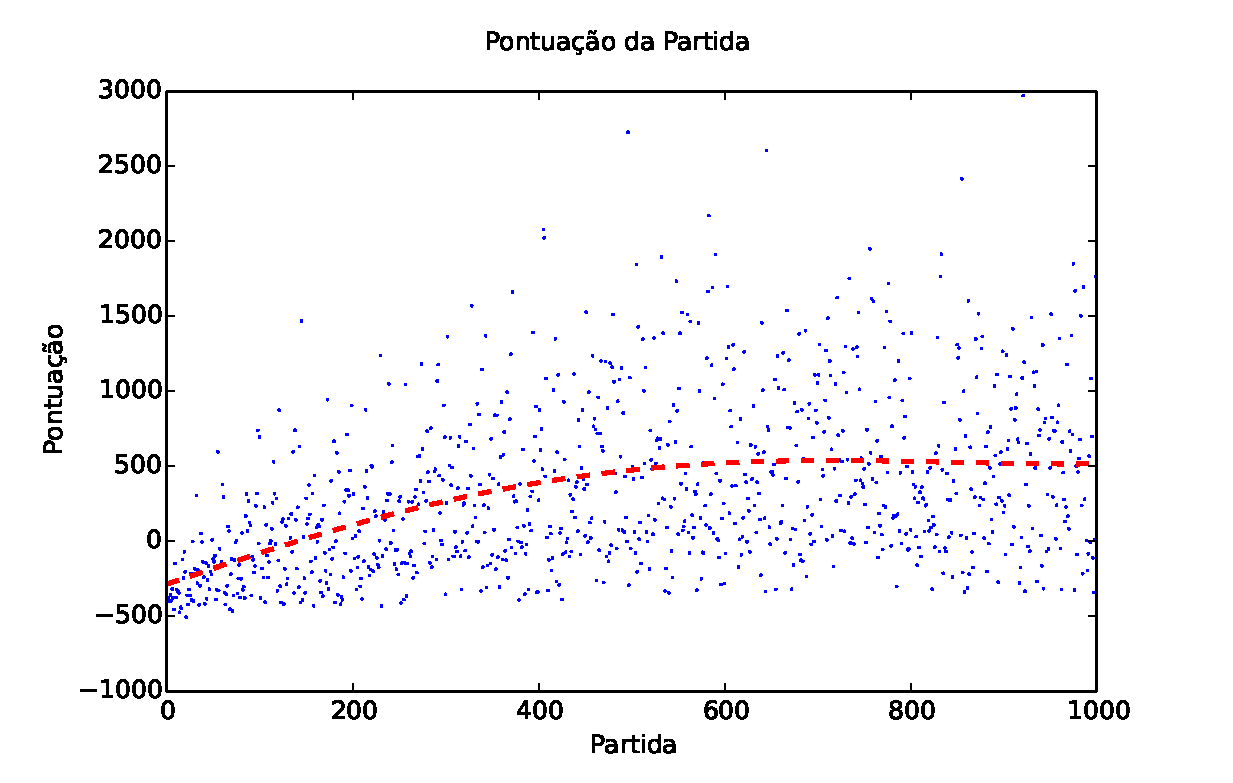
\includegraphics[width=\linewidth]{images/3_behaviors_original_map/match_scores____pol}
    \caption{Escolha de comportamentos por partida.}
    \label{img:3ComportamentosMapaOriginal:PontuacaoPorPartida}
\end{figure}

Essa função é ascendente e tende a uma constante. A média de pontos feita, após a conclusão do treinamento:

$$ mean \left( score \right) = 542.68488746 $$

Sendo a média de escolha pelo algorítmo de aprendizagem dos comportamentos:

$$ mean \left( Ficar\_Parado \right) = 0.183279742765 $$
$$ mean \left( Comer \right) = 164.572347267 $$
$$ mean \left( Fugir \right) = 3.26688102894 $$


\subsection{Discussão}

É possível ver que o algoritmo, nesse experimento, deu preferência à ação de comer, algumas vezes sendo ``super confiante''. Isso é explicado pela facilidade que o agente tem de receber pontos nesse ambiente, tendo mais raro encontro com fantasmas. Além disso, o fato de nesse mapa ele muitas vezes pegar uma Cápsula enquanto está executando a ação de comer, o permitindo comer fantasmas e receber pontos por isso, valoriza essa ação.


\section{5 Comportamentos no mapa pequeno (Teste 3)}

Nesse experimento%
\footnote{Os parâmetros e o setup desse experimento estão melhor descritos no tópico \ref{subsection:5ComportamentosMapaPequeno}.%
}, diferente dos anteriores, utilizamos 5 comportamentos. 

$$ B = \{Ficar\_Parado, Comer, Fugir, \textit{Comer\_Cápsula}, \textit{Caçar} \} $$

Usamos como vetor de características $ f $:

\begin{equation}
	\renewcommand\arraystretch{1.5}
	\begin{array}{r l}
		Bias: & f_1 \left( a, u \right) = 1.0 \\
		Dist. Comida: & f_2 \left( a, u \right) = \frac{\displaystyle 1}{\displaystyle ObterCaracteristicaDistanciaComida \left( a \right)} \\
		Dist. Capsula: & f_3 \left( a, u \right) = \frac{\displaystyle 1}{\displaystyle ObterCaracteristicaDistânciaCapsula \left( a \right)} \\
		Prob. Capsula Existir: & f_4 \left( a, u \right) = ObterCaracteristicaProbExistirCapsula \left( a \right) \\
		Prob. Fantasma Branco Existir: & f_5 \left( a, u \right) = ObterCaracteristicaProbExistirFantasmaBranco \left( a \right) \\
		Prob. Fantasma Por Perto: & f_6 \left( a, u \right) = ObterCaracteristicaProbFantasmas \left( a \right) \\
		Prob. Fantasma Branco Por Perto: & f_7 \left( a, u \right) = ObterCaracteristicaProbFantasmasBrancos \left( a \right)
	\end{array}
\end{equation}

Realizamos o treinamento ao longo de 2700 partidas, sendo que a exploração gulosa (\textit{greedy exploration}) foi executada até a partida 1500. Após terminado o treinamento utilizamos 300 partidas para avaliar e obter dados sobre o algoritmo treinado.


\subsection{Resultados e Análise}

Nas figuras à seguir, de \ref{img:5ComportamentosMapaPequeno:PesoBias} a \ref{img:5ComportamentosMapaPequeno:PesoProbFantasmaBrancoPorPerto}, temos os gráficos de como os valores dos pesos $ \omega_i $ evoluem com o tempo, para cada um dos comportamentos.

\begin{figure}[H]
	\centering
	\begin{subfigure}[t]{.5\textwidth}
		\centering
		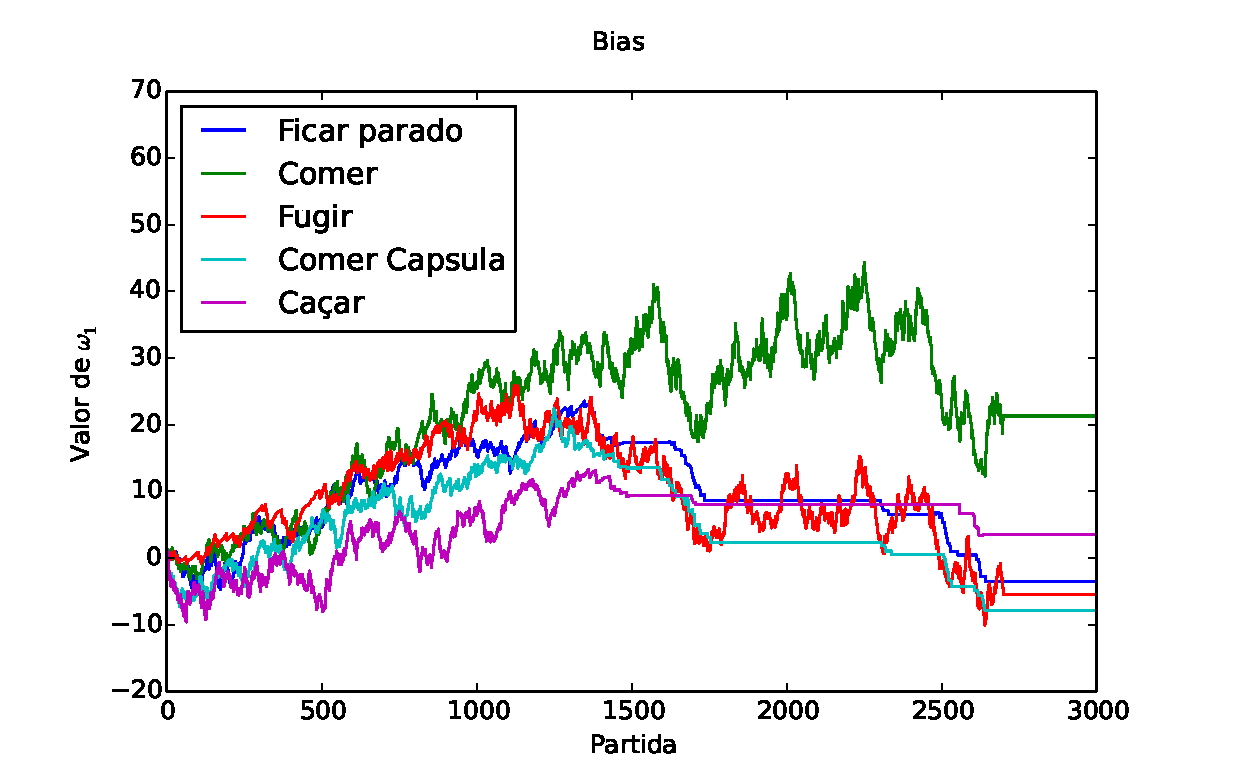
\includegraphics[width=\linewidth]{images/5_behaviors_small_map/weights____pol__Bias}
		\caption{Bias}
		\label{img:5ComportamentosMapaPequeno:PesoBias}
	\end{subfigure}%
	\begin{subfigure}[t]{.5\textwidth}
		\centering
		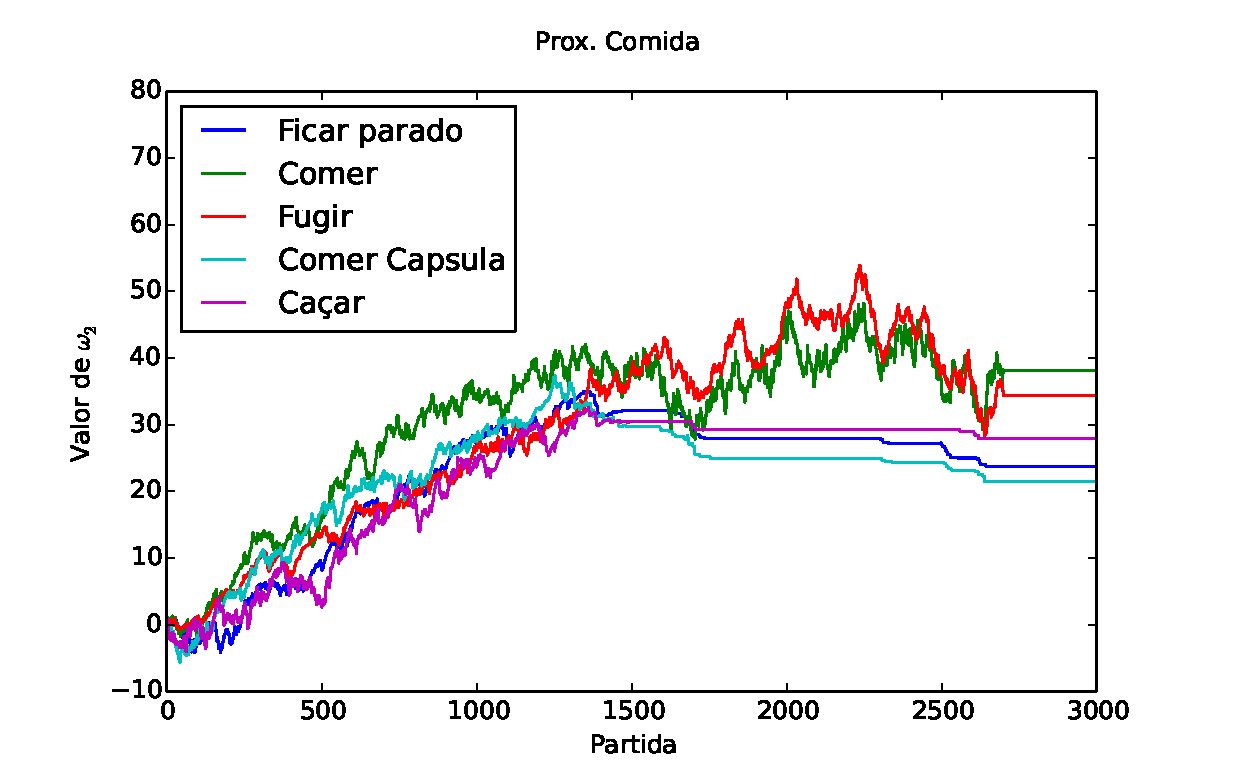
\includegraphics[width=\linewidth]{images/5_behaviors_small_map/weights____pol__DistComida}
		\caption{Proximidade para Comida}
		\label{img:5ComportamentosMapaPequeno:PesoDistComida}
	\end{subfigure}
	\caption{Evolução dos pesos $ \omega_1 $ e $ \omega_2 $}
	\label{img:5ComportamentosMapaPequeno:PesoBiasAndDistComida}
\end{figure}

\begin{figure}[H]
	\centering
	\begin{subfigure}[t]{.5\textwidth}
		\centering
		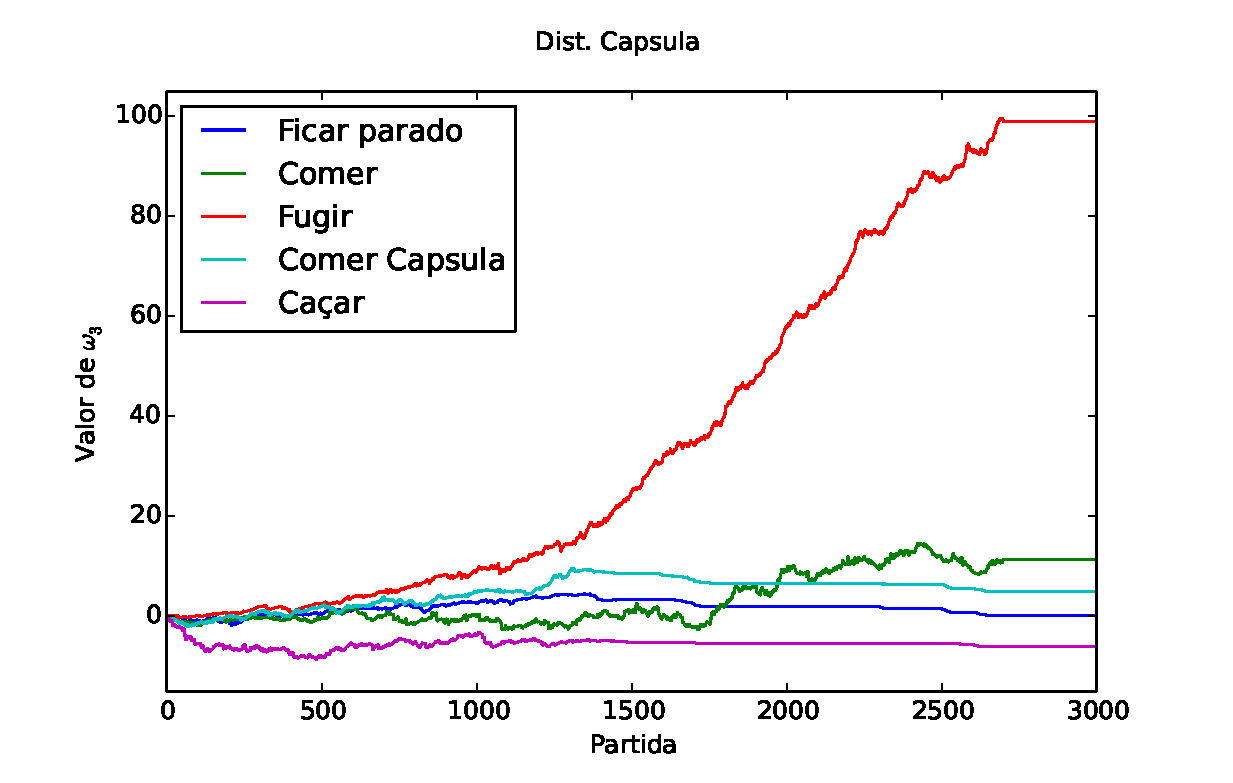
\includegraphics[width=80mm]{images/5_behaviors_small_map/weights____pol__DistCapsula}
		\caption{Proximidade para Cápsula}
		\label{img:5ComportamentosMapaPequeno:PesoDistCapsula}
	\end{subfigure}%
	\begin{subfigure}[t]{.5\textwidth}
		\centering
		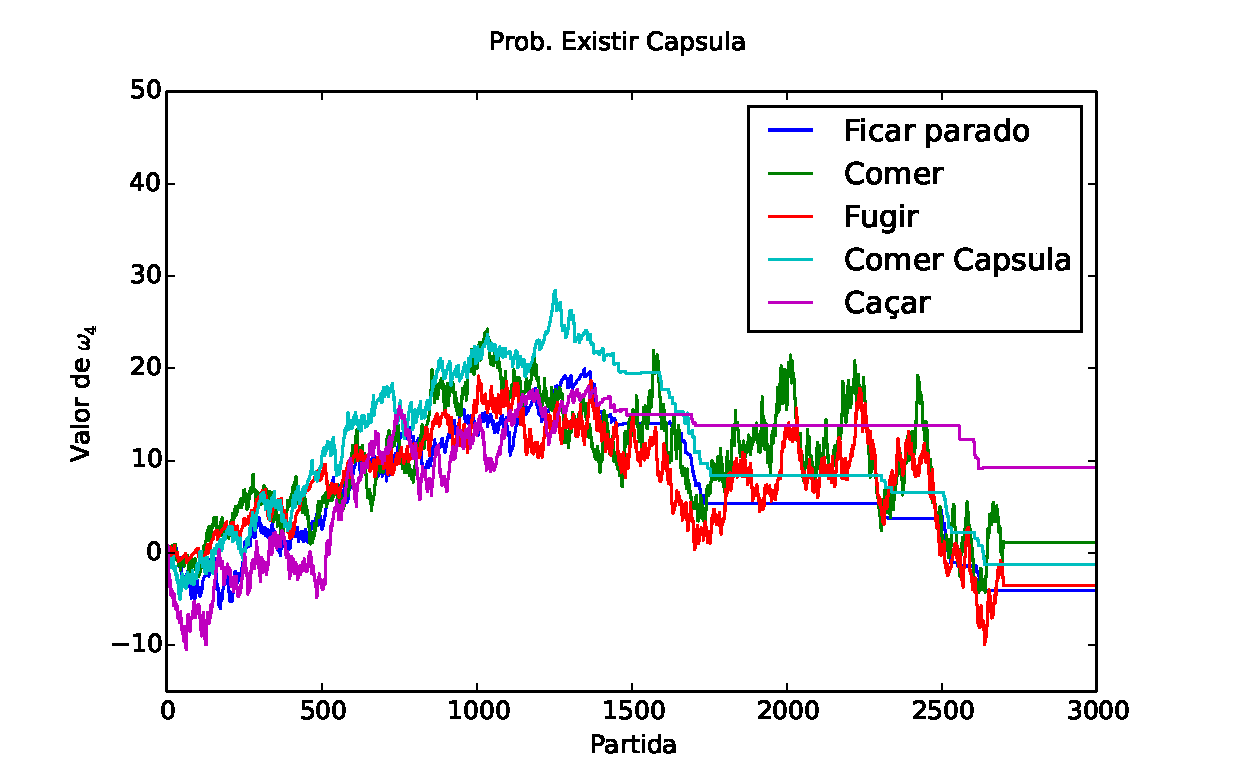
\includegraphics[width=80mm]{images/5_behaviors_small_map/weights____pol__ProbExistirCapsula}
		\caption{Probabilidade de uma Cápsula ainda Existir}
		\label{img:5ComportamentosMapaPequeno:PesoProbCapsulaExistir}
	\end{subfigure}
	\caption{Evolução dos pesos $ \omega_3 $ e $ \omega_4 $}
	\label{img:5ComportamentosMapaPequeno:PesoDistCapsulaOuProbCapsulaExistir}
\end{figure}

\begin{figure}[H]
	\centering
	\begin{subfigure}[t]{.5\textwidth}
		\centering
		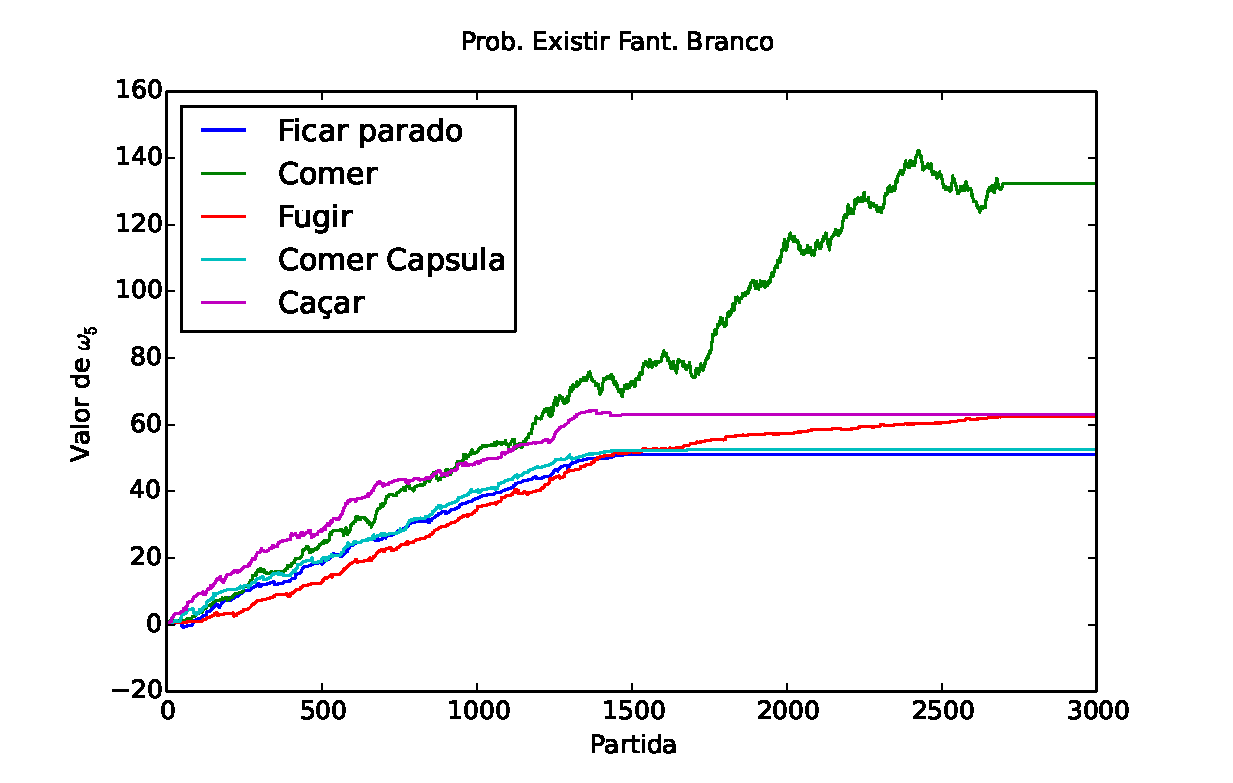
\includegraphics[width=80mm]{images/5_behaviors_small_map/weights____pol__ProbExistirFantBranco}
		\caption{Probabilidade de Fantasma Branco Existir}
		\label{img:5ComportamentosMapaPequeno:PesoProbFantasmaBrancoExistir}
	\end{subfigure}%
	\begin{subfigure}[t]{.5\textwidth}
		\centering
		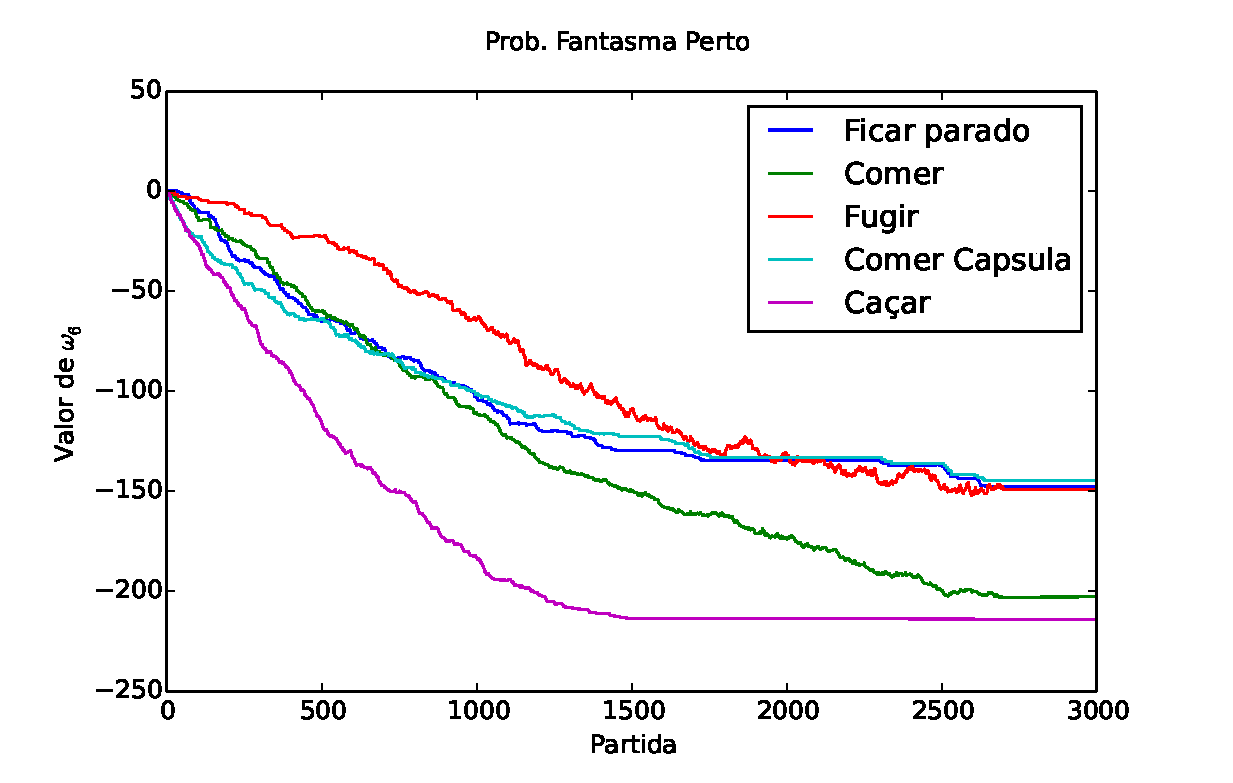
\includegraphics[width=\linewidth]{images/5_behaviors_small_map/weights____pol__ProbFantasmaPerto}
		\caption{Probabilidade de Fantasma por Perto}
		\label{img:5ComportamentosMapaPequeno:PesoProbFantasmaPorPerto}
	\end{subfigure}
	\caption{Evolução dos pesos $ \omega_5 $ e $ \omega_6 $}
	\label{img:5ComportamentosMapaPequeno:PesoProbFantasmaBrancoExistirOuNormalPerto}
\end{figure}

\begin{figure}[H]
	\centering
	\begin{subfigure}[t]{.5\textwidth}
		\centering
		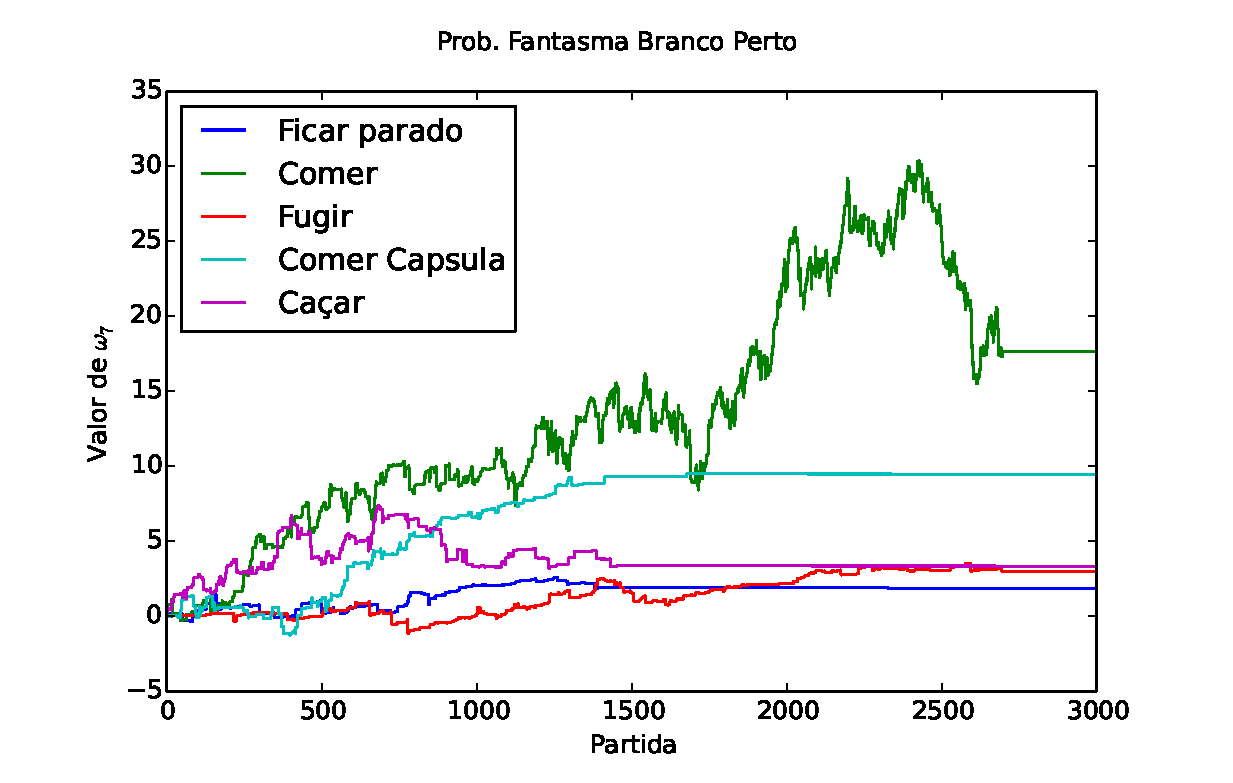
\includegraphics[width=80mm]{images/5_behaviors_small_map/weights____pol__ProbFantasmaBrancoPerto}
		\caption{Probabilidade de Fantasma Branco por Perto}
	\end{subfigure}%
	\caption{Evolução do peso $ \omega_7 $}
	\label{img:5ComportamentosMapaPequeno:PesoProbFantasmaBrancoPorPerto}
\end{figure}

Nesse experimento é mais difícil de fazer análise dos pesos, pois temos agora 7 pesos para comparar. Algumas características são fáceis de entender, por exemplo, ter um fantasma normal por perto é muito ruim quando se está comendo, e pior ainda quando se está caçando. Por outro lado $ Fugir $ ou $ Comer\_Capsula $ são boas alternativas nesse caso.

Para outras caracteríticas, é mais complexo entender o comportamento de seus pesos. A característica $ Prob Fantasma Branco Perto $, por exemplo, tem maior peso para $ Comer $ que para $ \textit{Caçar} $. Isso se dá, em boa parte, pela natureza probabilística do sistema. Como há uma probabilidade de esse fantasma não estar realmente branco, caçar pode não ser uma solução tão boa quanto ignorar os fantasmas e escolher o comportamento de $ Comer $.

Plotando o número de vezes que cada comportamentos é escolhido por partida para esse experimento, eles formam a nuvem exposta na figura \ref{img:5ComportamentosMapaPequeno:ComportamentosEscolhidos}.

\begin{figure}[H]
    \centering
    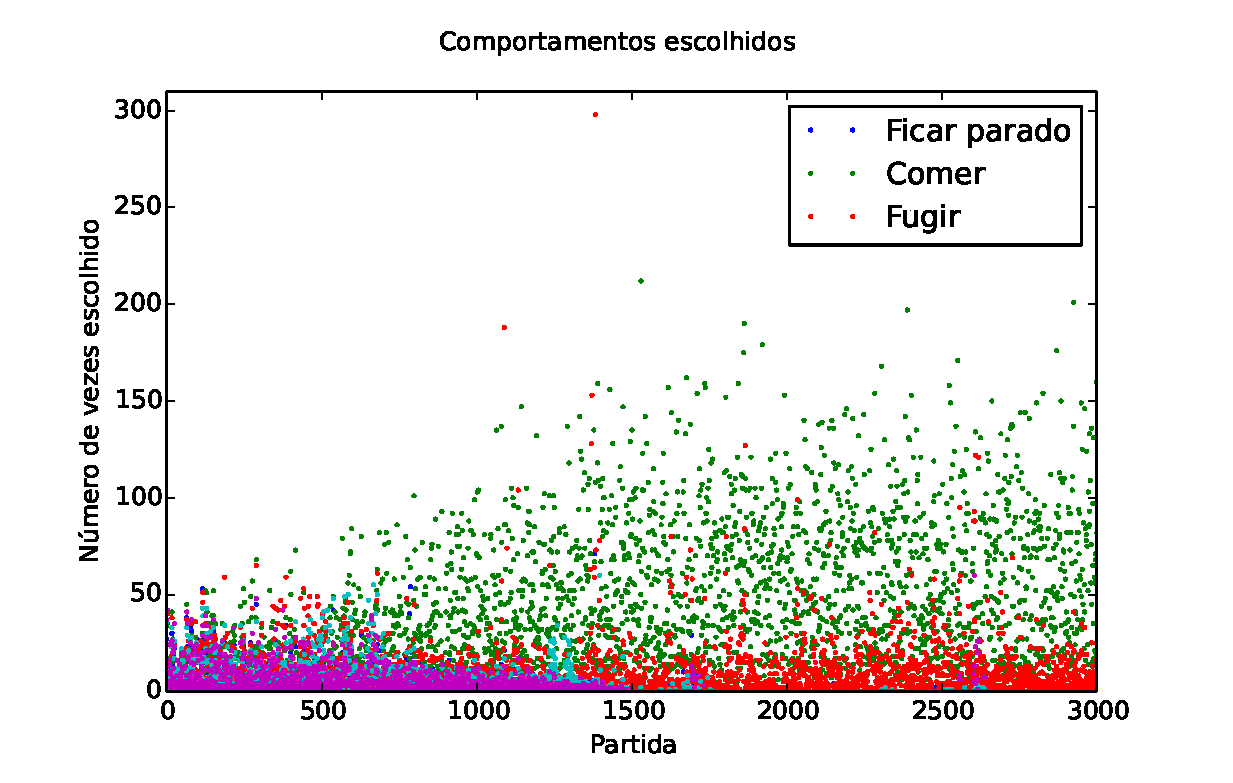
\includegraphics[width=\linewidth]{images/5_behaviors_small_map/chosen_behaviors}
    \caption{Escolha de comportamentos por partida.}
    \label{img:5ComportamentosMapaPequeno:ComportamentosEscolhidos}
\end{figure}

Novamente, para ter uma visualização melhor achamos um polinômio que represente essa nuvem de pontos, utilizando o método dos mínimos quadrados. Para um polinômio de quarto grau essa curva fica como a descrita na figura \ref{img:5ComportamentosMapaPequeno:ComportamentosEscolhidosPolinômio}.

\begin{figure}[H]
    \centering
    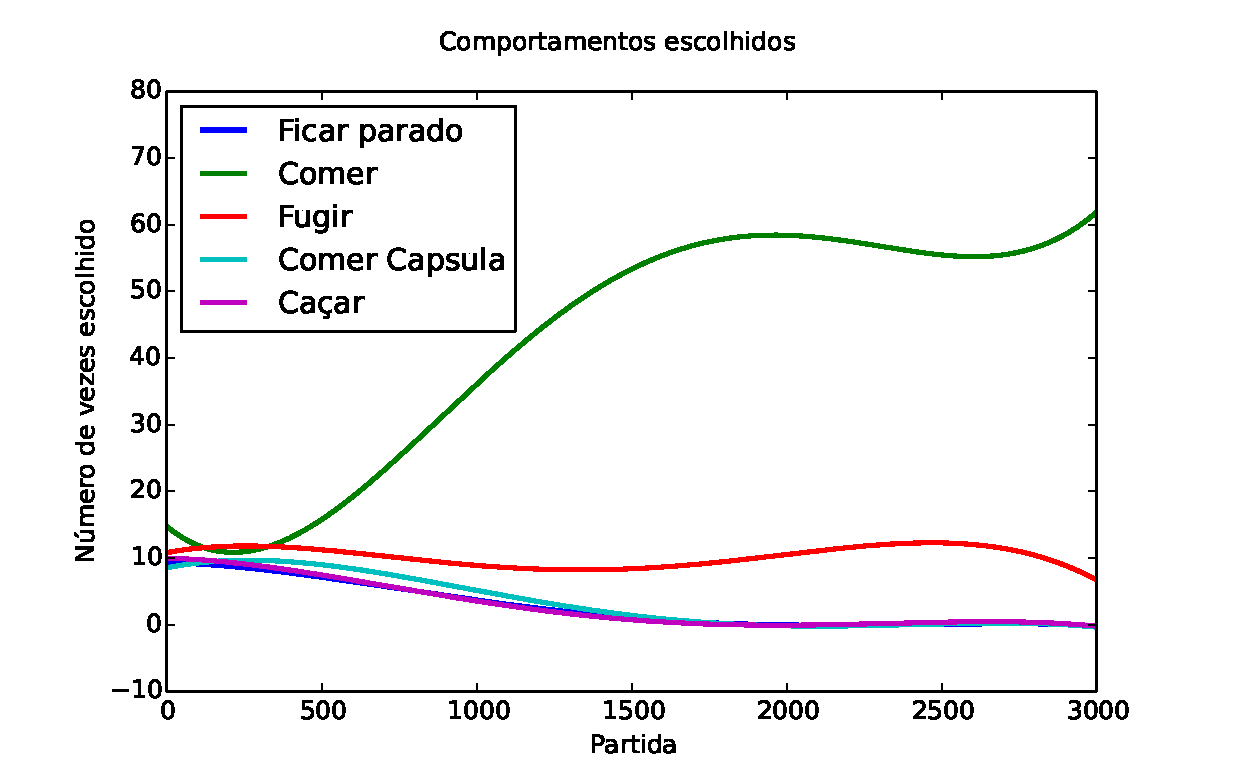
\includegraphics[width=\linewidth]{images/5_behaviors_small_map/chosen_behaviors_pol}
    \caption{Escolha de comportamentos por partida.}
    \label{img:5ComportamentosMapaPequeno:ComportamentosEscolhidosPolinômio}
\end{figure}

Nesse experimento, o comportamento $ Comer $ novamente tem o maior número de execuções, sendo $ Fugir $ o único que continua sendo executado até o final. Isso pode ser justificado por um fato não esperado, observado no experimento. O algoritmo ``percebeu'' que muitas das vezes que o comportamento $ Fugir $ é executado, o agente foge para cima da Cápsula, não só evitando o fantasma, mas servindo de substituto ao comportamento $ Comer\_Capsula $. Por isso o peso $ \omega_3 $, da característica $ Prox. Capsula $, é máximo para esse comportamento. Além disso, o comportamento $ Comer $, além de ir atrás da comida, muitas vezes acaba indo em direção a um fantasma branco nesse mapa pequeno.

A pontuação para cada partida pode ser vista na imagem à seguir, \ref{img:5ComportamentosMapaPequeno:PontuacaoPorPartida}. Novamente aproximamos esses dados por um polinômio de terceiro grau, utilizando o método dos mínimos quadrado.

\begin{figure}[H]
    \centering
    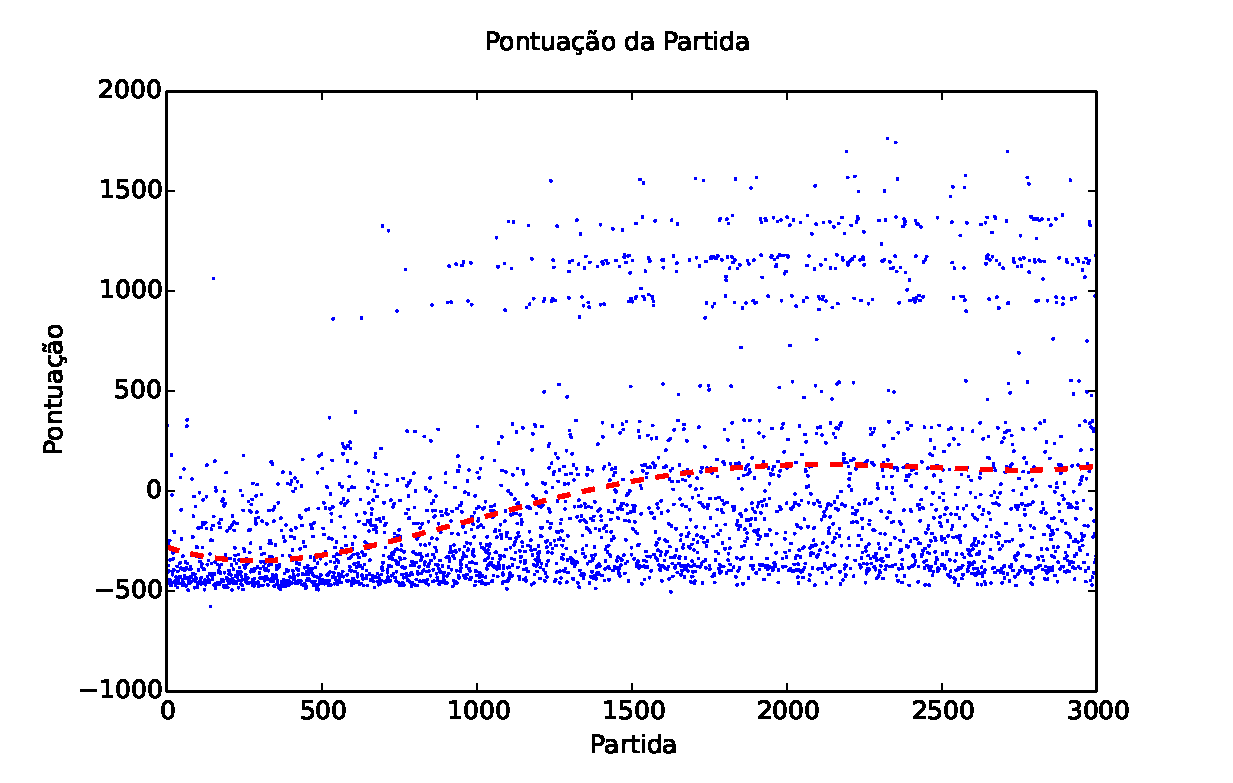
\includegraphics[width=\linewidth]{images/5_behaviors_small_map/match_scores____pol}
    \caption{Escolha de comportamentos por partida.}
    \label{img:5ComportamentosMapaPequeno:PontuacaoPorPartida}
\end{figure}

Exceto pelo inicio do experimento, aproximadamente as primeiras trezentas partidas, a pontuação aumenta durante todo o treinamento. A média de pontos feita, após a conclusão do treinamento:

$$ mean \left( score \right) = 143.93 $$

Sendo a média de escolha por partida dos comportamentos:

$$ mean \left( Ficar\_Parado \right) = 0.0 $$
$$ mean \left( Comer \right) = 59.10 $$
$$ mean \left( Fugir \right) = 8.35 $$
$$ mean \left( Comer\_Capsula \right) = 0.0 $$
$$ mean \left( \textit{Caçar} \right) = 0.0 $$


\subsection{Discussão}

O algoritmo, nesse experimento, após completo o treinamento, escolheu somente os comportamentos $ Comer $ e $ Fugir $, mesmo em posse dos outros. Isso pode ser explicado, em parte devido a particularidades encontradas no mapa, que não eram esperadas a princípio, e em parte pela natureza probabilística do sistema, o que dificulta se ter uma certeza de os fantasmas estarem brancos.


\section{5 Comportamentos no mapa original (Teste 4)}

Nesse experimento%
\footnote{Os parâmetros e o setup desse experimento estão melhor descritos no tópico \ref{subsection:5ComportamentosMapaOriginal}.%
}, como no anterior, utilizamos 5 comportamentos. 

$$ B = \{Ficar\_Parado, Comer, Fugir, \textit{Comer\_Cápsula}, \textit{Caçar} \} $$

E utilizamos como vetor de características $ f $:

\begin{equation}
\renewcommand\arraystretch{1.5}
	\begin{array}{r l}
		Bias: & f_1 \left( a, u \right) = 1.0 \\
		Dist. Comida: & f_2 \left( a, u \right) = \frac{\displaystyle 1}{\displaystyle ObterCaracteristicaDistanciaComida \left( a \right)} \\
		Dist. Capsula: & f_3 \left( a, u \right) = \frac{\displaystyle ObterCaracteristicaProbExistirCapsula \left( a \right)}{\displaystyle ObterCaracteristicaDistânciaCapsula \left( a \right)} \\
		Prob. Fantasma Branco Existir: & f_4 \left( a, u \right) = ObterCaracteristicaProbExistirFantasmaBranco \left( a \right) \\
		Prob. Fantasma Por Perto: & f_5 \left( a, u \right) = ObterCaracteristicaProbFantasmas \left( a \right) \\
		Prob. Fantasma Branco Por Perto: & f_6 \left( a, u \right) = ObterCaracteristicaProbFantasmasBrancos \left( a \right)
	\end{array}
\end{equation}

Realizamos o treinamento ao longo de 700 partidas, sendo que a exploração gulosa (\textit{greedy exploration}) foi executada até a partida 500. Após terminado o treinamento utilizamos 300 partidas para avaliar e obter dados sobre o algoritmo treinado.


\subsection{Resultados e Análise}

Nas figuras à seguir, de \ref{img:5ComportamentosMapaOriginal:PesoBiasAndDistComida} a \ref{img:5ComportamentosMapaOriginal:PesoProbFantasmaBrancoExistirOuNormalPerto}, temos os gráficos de como os valores dos pesos $ \omega_i $ evoluem com o tempo, para cada um dos comportamentos.

\begin{figure}[H]
	\centering
	\begin{subfigure}[t]{.5\textwidth}
		\centering
		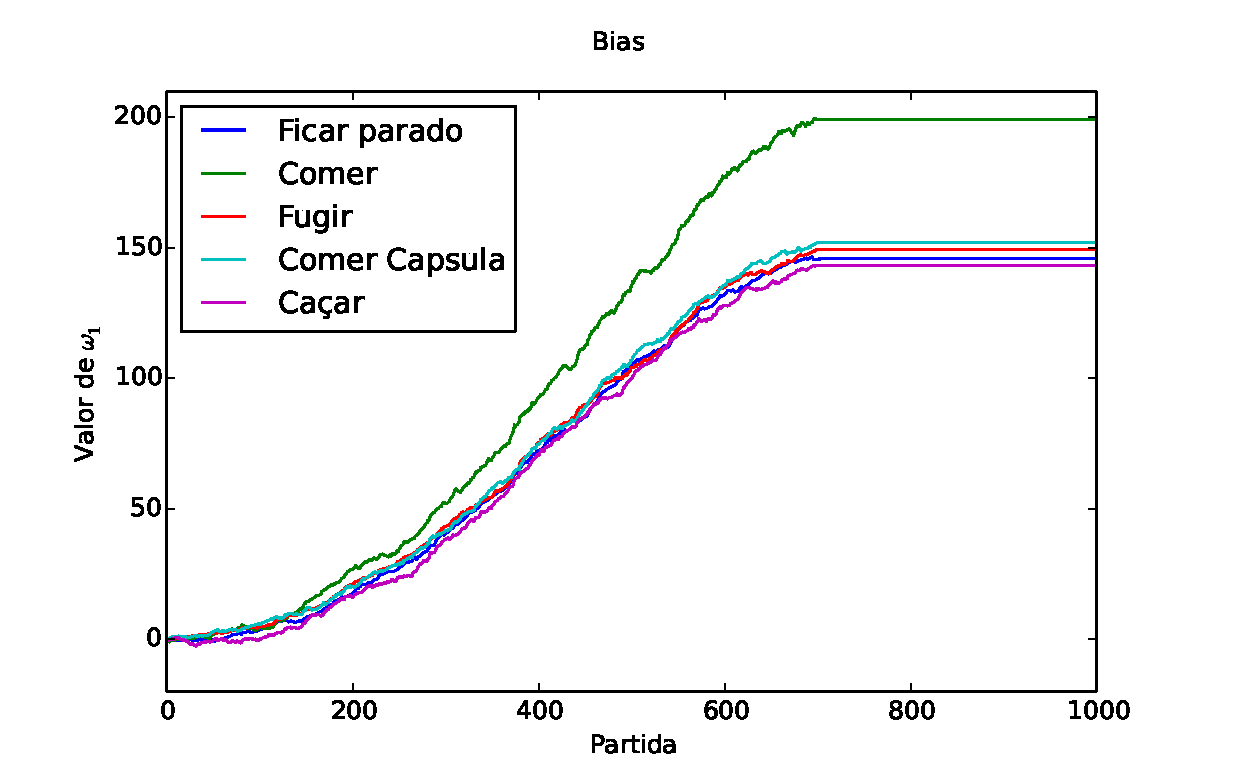
\includegraphics[width=\linewidth]{images/5_behaviors_original_map/weights____pol__Bias}
		\caption{Bias}
		\label{img:5ComportamentosMapaOriginal:PesoBias}
	\end{subfigure}%
	\begin{subfigure}[t]{.5\textwidth}
		\centering
		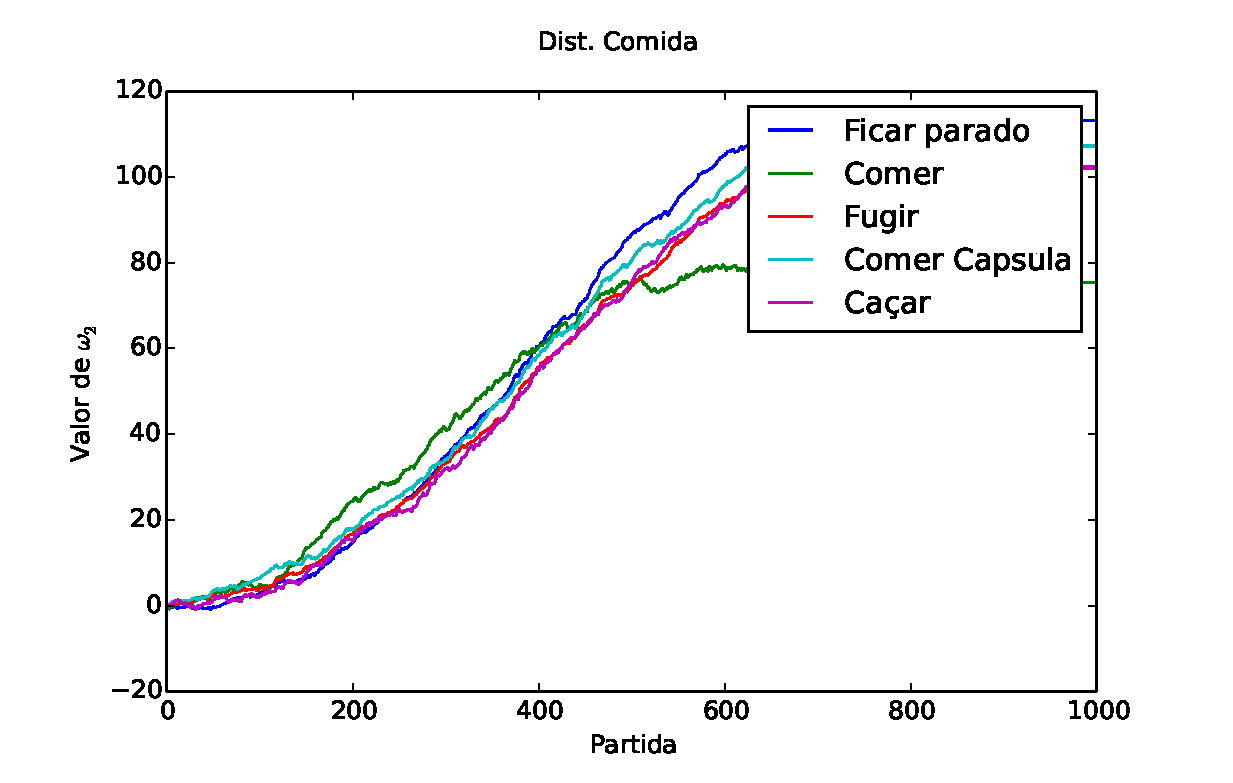
\includegraphics[width=\linewidth]{images/5_behaviors_original_map/weights____pol__DistComida}
		\caption{Proximidade para Comida}
		\label{img:5ComportamentosMapaOriginal:PesoDistComida}
	\end{subfigure}
	\caption{Evolução dos pesos $ \omega_1 $ e $ \omega_2 $}
	\label{img:5ComportamentosMapaOriginal:PesoBiasAndDistComida}
\end{figure}

\begin{figure}[H]
	\centering
	\begin{subfigure}[t]{.5\textwidth}
		\centering
		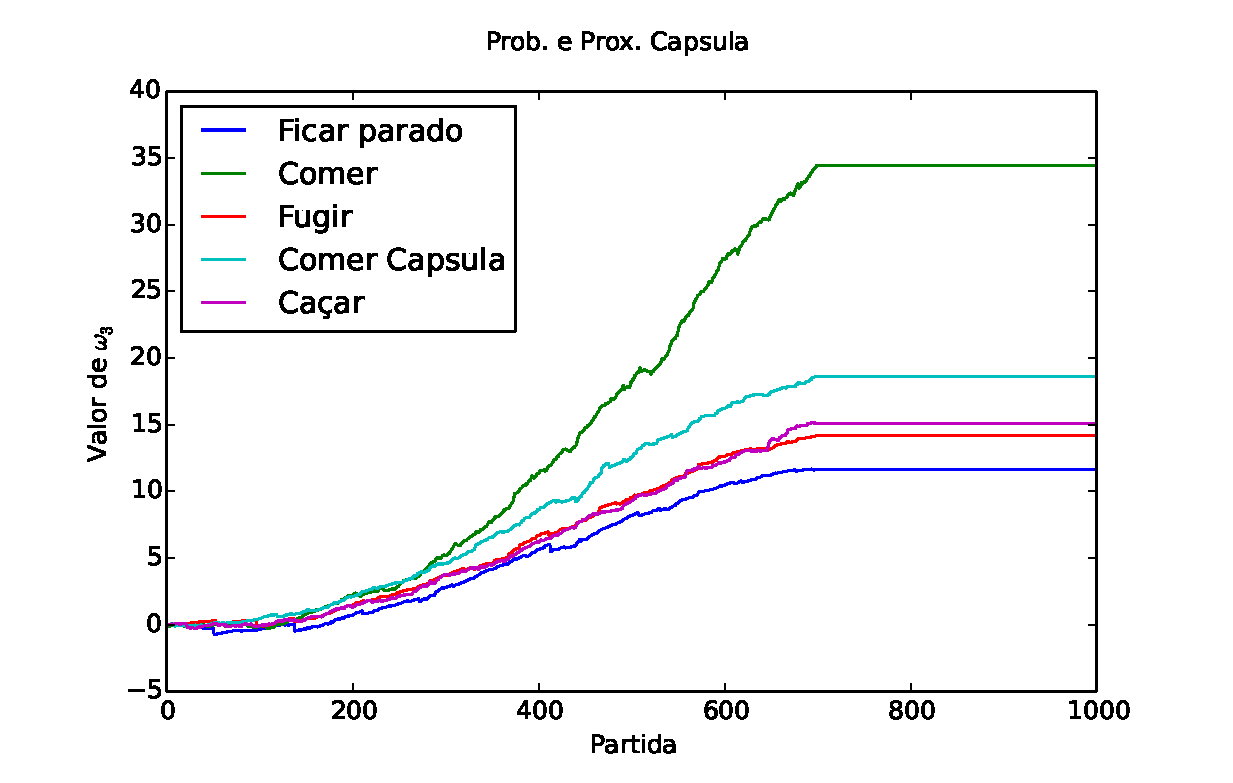
\includegraphics[width=80mm]{images/5_behaviors_original_map/weights____pol__DistCapsula}
		\caption{Proximidade para Cápsula}
		\label{img:5ComportamentosMapaOriginal:PesoDistCapsula}
	\end{subfigure}%
	\begin{subfigure}[t]{.5\textwidth}
		\centering
		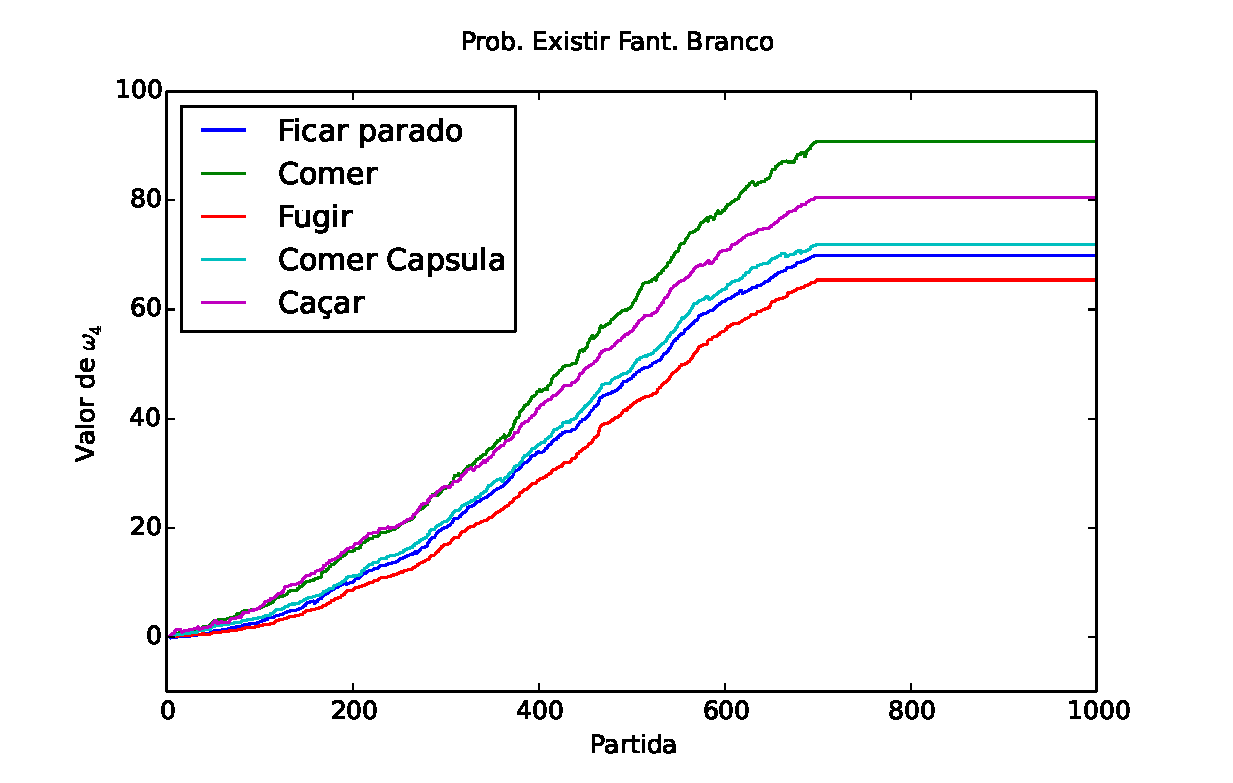
\includegraphics[width=80mm]{images/5_behaviors_original_map/weights____pol__ProbExistirCapsula}
		\caption{Probabilidade de Fantasma Branco Existir}
		\label{img:5ComportamentosMapaOriginal:PesoProbFantasmaBrancoExistir}
	\end{subfigure}
	\caption{Evolução dos pesos $ \omega_3 $ e $ \omega_4 $}
	\label{img:5ComportamentosMapaOriginal:PesoDistCapsulaOuProbCapsulaExistir}
\end{figure}

\begin{figure}[H]
	\centering
	\begin{subfigure}[t]{.5\textwidth}
		\centering
		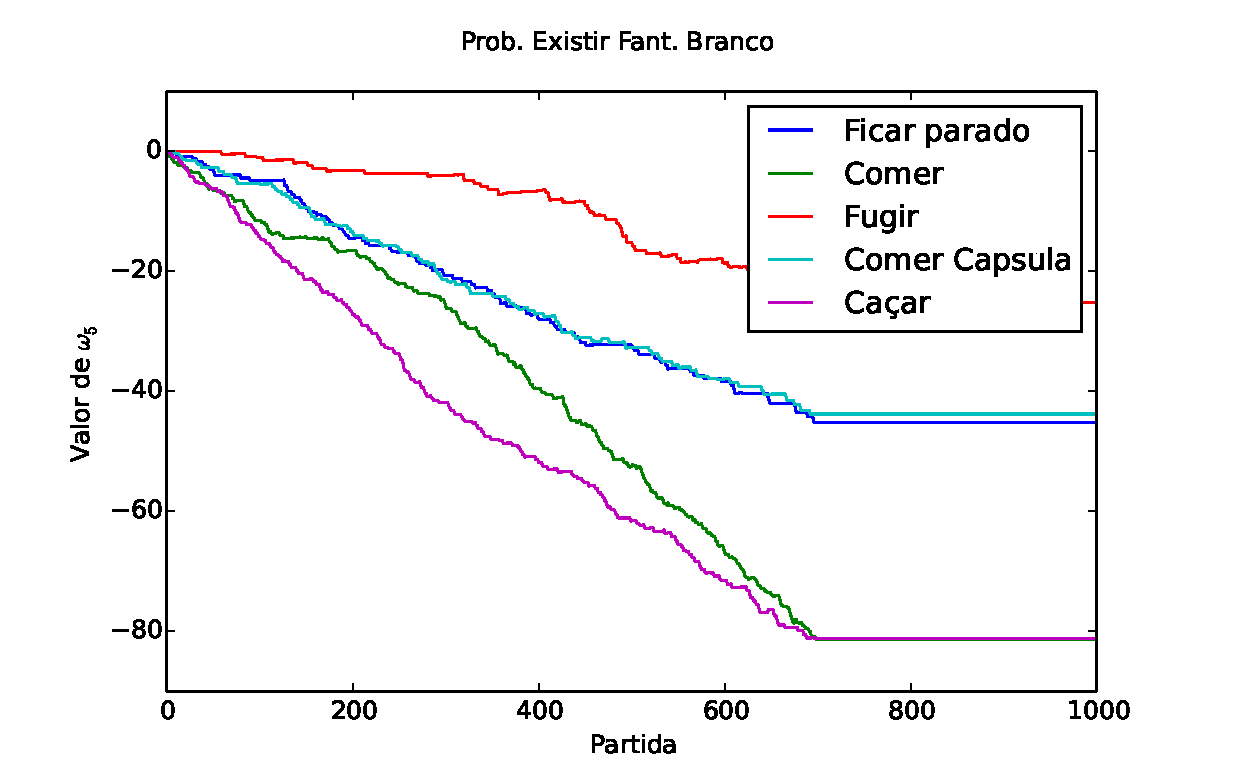
\includegraphics[width=80mm]{images/5_behaviors_original_map/weights____pol__ProbExistirFantBranco}
		\caption{Probabilidade de Fantasma por Perto}
		\label{img:5ComportamentosMapaOriginal:PesoProbFantasmaPorPerto}
	\end{subfigure}%
	\begin{subfigure}[t]{.5\textwidth}
		\centering
		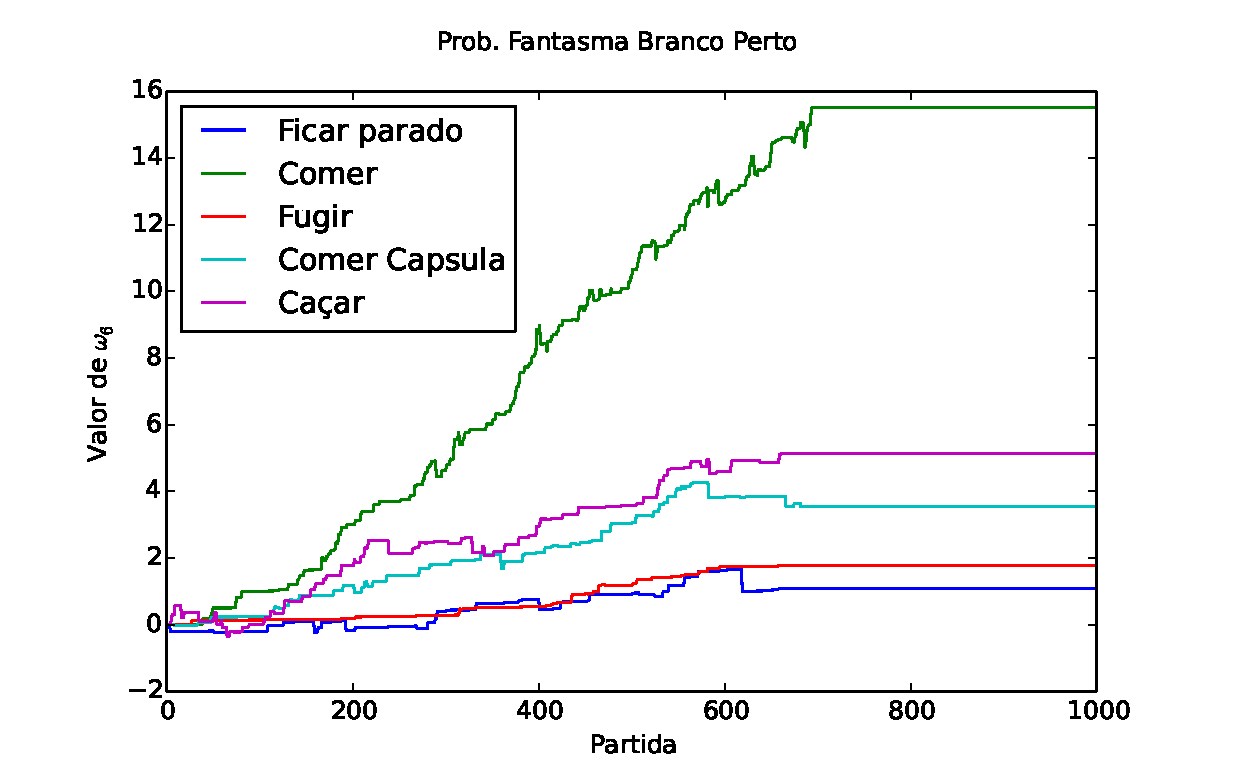
\includegraphics[width=\linewidth]{images/5_behaviors_original_map/weights____pol__ProbFantasmaPerto}
		\caption{Probabilidade de Fantasma Branco por Perto}
	\label{img:5ComportamentosMapaOriginal:PesoProbFantasmaBrancoPorPerto}
	\end{subfigure}
	\caption{Evolução dos pesos $ \omega_5 $ e $ \omega_6 $}
	\label{img:5ComportamentosMapaOriginal:PesoProbFantasmaBrancoExistirOuNormalPerto}
\end{figure}

Nesse experimento temos 6 pesos diferentes. Podemos ver que a Bias alcança os maiores valores, assim como no outro teste para esse mesmo mapa. Isso acontece devido ao fato de esse mapa ser mais ``fácil'', o que faz com que todos os comportamentos tenham valor maior.

Assim como no teste 3, também com 5 comportamentos, temos pesos diferentes do esperado para a característica $ \textit{Proximidade Cápsula} $, mas dessa vez o comportamento que tem maior valor para ela é $ Comer $. Isso ocorre pois, nesse mapa, $ Comer $, quando escolhido próximo a uma cápsula, quase sempre leva o agente a comê-la.

Vemos também que os pesos $ \omega_4 $ e $ \omega_6 $, $ \textit{Prob. Existir Fantasma Branco} $ e $ \textit{Prob. Fantasma Braco Perto} $, respectivamente, tem maior valor também para $ Comer $. O que reflete que $ Comer $ nesse mapa, além de levar a pegar comidas, por ser indiferente aos fantasmas, é preferível nesse caso a procurar ativamente por ele.

Como para os outros experimentos, plotando o número de vezes que cada comportamentos é escolhido por partida para esse experimento, eles formam a nuvem exposta na figura \ref{img:5ComportamentosMapaOriginal:ComportamentosEscolhidos}.

\begin{figure}[H]
    \centering
    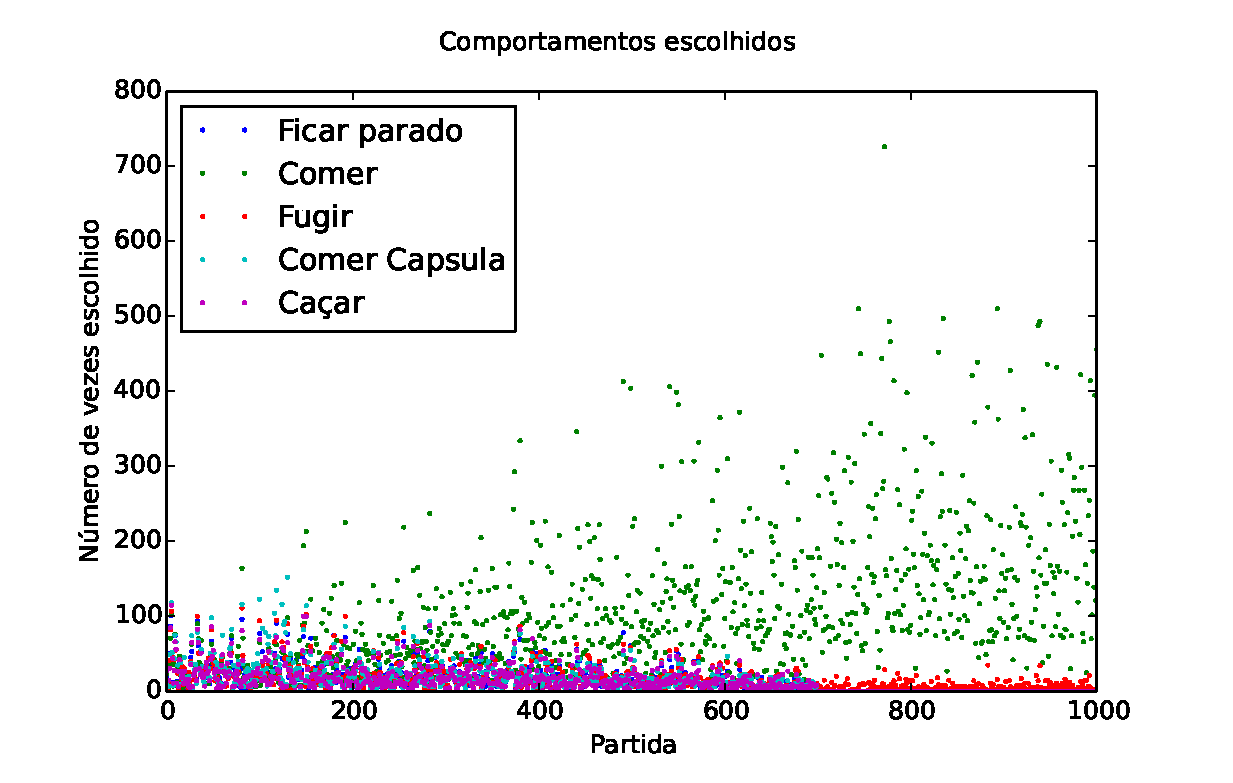
\includegraphics[width=\linewidth]{images/5_behaviors_original_map/chosen_behaviors}
    \caption{Escolha de comportamentos por partida.}
    \label{img:5ComportamentosMapaOriginal:ComportamentosEscolhidos}
\end{figure}

Novamente, para ter uma visualização melhor achamos um polinômio que represente essa nuvem de pontos, utilizando o método dos mínimos quadrados. Para um polinômio de quarto grau essa curva fica como a descrita na figura \ref{img:5ComportamentosMapaOriginal:ComportamentosEscolhidosPolinômio}.

\begin{figure}[H]
    \centering
    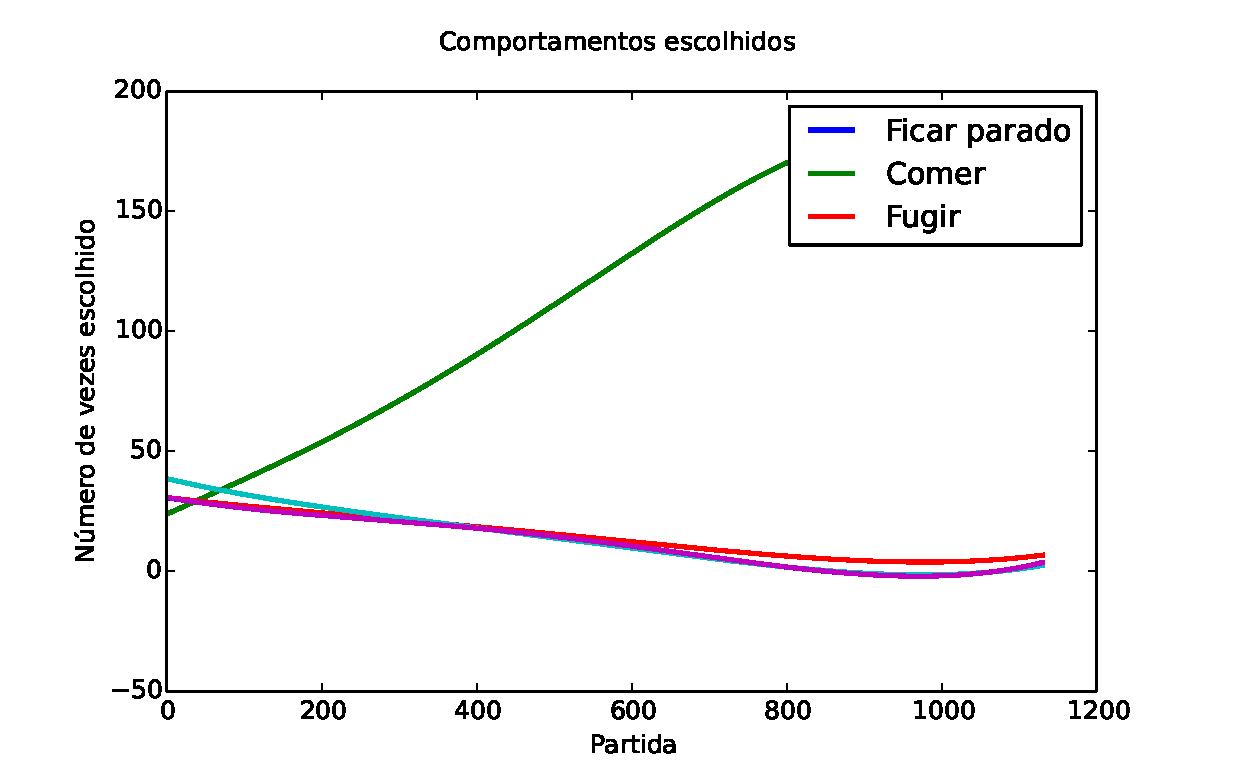
\includegraphics[width=\linewidth]{images/5_behaviors_original_map/chosen_behaviors_pol}
    \caption{Escolha de comportamentos por partida.}
    \label{img:5ComportamentosMapaOriginal:ComportamentosEscolhidosPolinômio}
\end{figure}

Como para os outros experimentos, o comportamento $ Comer $ foi o mais escolhido, seguido por $ Fugir $. Assim como para o outro experimento com 5 comportamentos, após completo o treinamento somente esses dois comportamentos são utilizados. Isso novamente se deve a uma característica do mapa, em geral quando o agente está a uma pequena distância de uma cápsula, o comportamento $ Comer $ o leva na mesma direção que o $ \textit{Comer\_Cápsula} $.

A pontuação para cada partida pode ser vista na imagem à seguir, \ref{img:5ComportamentosMapaOriginal:PontuacaoPorPartida}. Novamente aproximamos esses dados por um polinômio de terceiro grau, utilizando o método dos mínimos quadrado.

\begin{figure}[H]
    \centering
    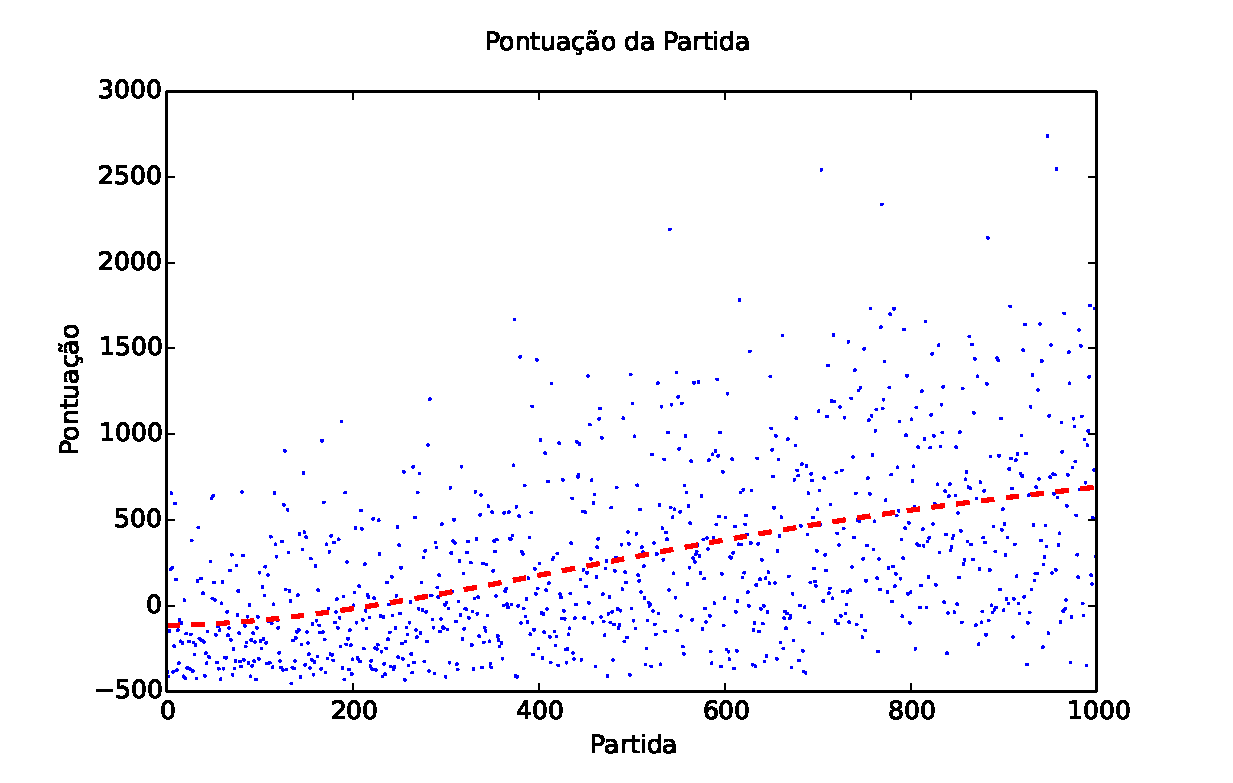
\includegraphics[width=\linewidth]{images/5_behaviors_original_map/match_scores____pol}
    \caption{Escolha de comportamentos por partida.}
    \label{img:5ComportamentosMapaOriginal:PontuacaoPorPartida}
\end{figure}

Essa curva mostra uma melhora na pontuação ao longo de todo o treinamento. A média de pontos feita, após a conclusão do treinamento:

$$ mean \left( score \right) = 619.20 $$

Sendo a média de escolha por partida dos comportamentos:

$$ mean \left( Ficar\_Parado \right) = 0.0 $$
$$ mean \left( Comer \right) = 181.04 $$
$$ mean \left( Fugir \right) = 5.29 $$
$$ mean \left( Comer\_Capsula \right) = 0.0 $$
$$ mean \left( \textit{Caçar} \right) = 0.0 $$


\subsection{Discussão}

Assim como para o teste anterior, o algoritmo escolheu somente os comportamentos $ Comer $ e $ Fugir $, mesmo em posse dos outros, após o treinamento estar completo. Isso pode ser explicado em parte devido a particularidades encontradas no mapa, que não eram esperadas a princípio, e em parte pela natureza probabilística do sistema, o que dificulta se ter uma certeza de os fantasmas estarem brancos.

Pode-se observar também que existe uma dificuldade do algoritmo de sair de um máximo local para alcançar um máximo global. Pelo fato de ele inicialmente perceber que é ruim ter uma probabilidade alta de possuir fantasmas normais por perto, ele não consegue aprender a escolher o comportamento $ \textit{Caçar} $ como seria desejado, mesmo para casos com alta probabilidade de os fantasmas estarem brancos.

\section{Discussão Geral}

O algoritmo, como esperado, teve comportamentos diferentes, para diferentes mapas, comportamentos e parâmetros.

Algumas coisas inesperadas foram observadas, por exemplo, nos terceiro e quarto casos de teste, mesmo só executando, ao final, dois comportamentos, $ Comer $ e $ Fugir $, os mesmo executados pelos dois primeiros experimentos, ele conseguiu uma média de pontos bastante superior. Isso se deve ao caso de uma característica, que parecia ter pouca relevância para esses dois comportamentos, ser mais importante que o esperado. Isso reforça a informação dada na Fundamentação Teórica, no tópico \ref{subsection:GeneralizaçãoParesEstadoAção}, que falava ``devemos escolher esses valores/características com cuidado para obter uma boa representação do nosso par estado-ação [...] ou podemos ter estados-ações com valores [...] parecidos, e, consequentemente, valores de $ Q \left( S, U \right) $ também parecidos, mas que são muito diferentes.''

O modelo obteve bons resultados, conseguindo fazer escolhas satisfatórias mesmo num sistema com alto erro de atuação e sensoriamento e sem ter nenhuma informação previa de como os comportamentos influenciariam seu desenpenho ou atuação. Mesmo com algumas características inesperadas encontradas, o algoritmo se comportou como desejado. Nos experimentos com o mapa clássico, por exemplo, ele aprende e valoriza muito mais a ação de comer, enquanto nos mapas pequenos ele é muito mais cauteloso.


\begin{comment}
Conclusões
\end{comment}
%TCIDATA{LaTeXparent=0,0,relatorio.tex}


\chapter{Conclusões} \label{Chap:Conclusoes}

O algoritmo teve o desempenho desejado e conseguiu aprender como utilizar os diferentes parâmetros para fazer boas escolhas num sistema estocástico. Ele apresentou, ainda, curvas  de aprendizagem diferentes para mapas diferentes, como é esperado.

Os testes mostram, também, que esse algoritmo consegue aprender características específicas dos mapas. Um exemplo é a percepção que um ou outro comportamento, ao ser invocado em uma parte específica do mapa, consegue ganhos que não são inerentes a ele.

O algoritmo, no entanto, possui algumas limitações, como, por exemplo, sua dificuldade para sair de um máximo local, para certas circunstâncias. Outra limitação é ter de se escolher os parâmetros manualmente, de forma que eles consigam descrever bem o sistema, tendo valores linearmente separáveis para diferentes comportamentos.

\section{Perspectivas Futuras}

Uma proposta que pode ser feita para evoluir esse trabalho é a utilização de uma rede neural no lugar da função de ganho atualmente utilizada. Com uma rede neural os parâmetros não teriam de ser escolhidos manualmente e relações mais complexas poderiam ser descobertas, a partir do espectro de probabilidades atual do sistema $ a \in A $.

Outro trabalho que pode ser feito é a criação de uma plataforma física em que esse sistema poderia ser testado fora de simulação, dando suporte para os robôs não se danificarem durante o processo de aprendizagem.


\begin{comment}
Bibliografia
\end{comment}


\renewcommand{\bibname}{REFERÊNCIAS BIBLIOGRÁFICAS} 
\addcontentsline{toc}{chapter}{REFERÊNCIAS BIBLIOGRÁFICAS} 

\bibliographystyle{abnt-num}
\bibliography{relatorio}


\begin{comment}
Anexos
\end{comment}


\anexos 
\makeatletter 
% não retirar estes comandos 
\renewcommand{\@makechapterhead}[1]{%
  {\parindent \z@ \raggedleft \setfontarial\bfseries          
\LARGE \thechapter. \space\space      
\uppercase{#1}\par     
\vskip 40\p@   
} 
} 
\makeatother

\begin{comment}
Anexo I: Diagramas esquemáticos 
\end{comment}


%TCIDATA{LaTeXparent=0,0,relatorio.tex}



\chapter{Diagramas Esquemáticos\label{AnEsquematicos}}


\refstepcounter{noAnexo}

\begin{comment}
Anexo II: Descriçao do CD
\end{comment}


%TCIDATA{LaTeXparent=0,0,relatorio.tex}



\chapter{Descrição do conteúdo do CD}

\label{AnCD} 

O CD segue a seguinte estrutura:
\begin{itemize}
\item leiame.pdf : Essa descrição do CD
\item \textbackslash{}template\_relatorio : Um template de Relatórios de
Graduação, já ajustado e configurado para uso no Lyx.
\item \textbackslash{}Rhino

\begin{itemize}
\item \textbackslash{}codigo : Pasta com uma versão comprimida do software
criado para controle do $\rhino$.
\item \textbackslash{}videos :

\begin{itemize}
\item homing.mov : Video do $\rhino$ executando o procedimento de \textit{homing}.
\end{itemize}
\item \textbackslash{}referencias: diversos manuais de fabricantes que possuem
informações relevantes usadas no desenvolvimento da plataforma.
\item \textbackslash{}matlab: \textit{script} do Matlab que lê os dados
obtidos no experimento com o $\rhino$ e cria os gráficos, para verificação.
\end{itemize}
\item Schunk

\begin{itemize}
\item \textbackslash{}codigo:

\begin{itemize}
\item \textbackslash{}simulacao modo insercao : código desenvolvido na linguagem
C utilizado para realizar a simulação da tarefa de controle no modo
de inserção.
\item \textbackslash{}simulacao modo posicionamento: código desenvolvido,
incluindo o simulador 3D, que realiza a simulação da tarefa de controle
no modo de controle de posição por sensor de força. O simulador também
realiza a outra tarefa de controle se configurado corretamente.
\end{itemize}
\item \textbackslash{}videos:

\begin{itemize}
\item posicionamento.avi : Vídeo do simulador 3D executando o controle de
posicionamento.
\end{itemize}
\item \textbackslash{}referencias: diversos manuais de fabricantes que possuem
informações relevantes.
\item \textbackslash{}modelagem: contém um arquivo .pdf com os parâmetros
$\dh$ obtidos nesse trabalho.
\item \textbackslash{}matlab: 

\begin{itemize}
\item \textbackslash{}simulacao modo insercao: a própria simulação no modo
de inserção.
\item \textbackslash{}simulacao modo posicionamento: \textit{script} do
Matlab que lê os dados obtidos no experimento de posicionamento e
cria os gráficos.\end{itemize}
\end{itemize}
\end{itemize}



\refstepcounter{noAnexo}

\begin{comment}
Anexo III: Programas Utilizados
\end{comment}


%TCIDATA{LaTeXparent=0,0,relatorio.tex}



\chapter{Programas utilizados}

Esse tipo de anexo é puramente opcional e recomendo bastante.

\label{AnFRHINO} 

Reunindo todas as referências obtidas, com um agradecimento especial
à Mariana C. Bernardes, alguns dos programas utilizados serão citados.
\begin{itemize}
\item Escrita do relatório:

\begin{itemize}
\item Usou-se o Lyx como ambiente de desenvolvimento para criar o texto
usando \TeX{}. Ele permite que se use o \TeX{} sem ter que se preocupar
demais com coisas pequenas, como gerenciamento de rótulos e facilita,
infinitamente, a criação de tabelas, matrizes, figuras etc.
\item Usou-se o inkscape para desenhar quadros e para adicionar setas e
textos nas figuras. A capacidade de exportar em .pdf com texto em
\TeX{} é fantástica.
\item Usou-se o Visio para desenho da maioria dos diagramas de blocos. Quando
símbolos \TeX{} foram necessários, exportou-se em .svg e adicionaram-se
os textos no inkscape. Em um dos blocos, usou-se o simulink.
\item Para gerenciamento da bibliografia, usou-se o JabRef. Ele também facilita
a organização da sua biblioteca de referências.
\end{itemize}
\item Simulação:

\begin{itemize}
\item Basicamente se usou o Matlab. O \textit{script }pode ser escrito para
que ele já imprima no .pdf. Assim, se algo for alterado na simulação,
basta apenas executá-la com esses comandos, que o relatório automaticamente
atualiza com as figuras corretas.
\end{itemize}
\item Ambiente de programação:

\begin{itemize}
\item Linux: No Linux escreveu-se usando o gedit e compilação com makefiles.
Não se podia arriscar instalar outro programa e impedir o funcionamento
correto do Xenomai.
\item Windows: Visual Studio. O debbuger ajuda muito no desenvolvimento,
principalmente quando se está trabalhando com alocação dinâmica.
\end{itemize}
\item Algumas bibliotecas específicas

\begin{itemize}
\item Matrix: Para operações com matrizes, usou-se a biblioteca gMatrix
do Professor Geovany A. Borges. A biblioteca já tem diversas funções
prontas e é fácil implementar sobre ela quando necessário.
\item Impressão para leitura no Matlab: gDataLogger do Professor Geovany
A. Borges, em geral. Essa biblioteca deixa transparente a maior parte
do processo, e facilita muito. No caso do simulador G3D, não se conseguiu
usar essa biblioteca, então outra forma foi encontrada. Não é complicado,
apenas realizar um fwrite() com o dado desejado e depois realizar
a leitura.\end{itemize}
\end{itemize}



\refstepcounter{noAnexo}

\begin{comment}
Acrescente mais anexos conforme julgar necessário.
\end{comment}

\end{document}
